\documentclass[twoside]{book}

% Packages required by doxygen
\usepackage{fixltx2e}
\usepackage{calc}
\usepackage{doxygen}
\usepackage[export]{adjustbox} % also loads graphicx
\usepackage{graphicx}
\usepackage[utf8]{inputenc}
\usepackage{makeidx}
\usepackage{multicol}
\usepackage{multirow}
\PassOptionsToPackage{warn}{textcomp}
\usepackage{textcomp}
\usepackage[nointegrals]{wasysym}
\usepackage[table]{xcolor}

% Font selection
\usepackage[T1]{fontenc}
\usepackage[scaled=.90]{helvet}
\usepackage{courier}
\usepackage{amssymb}
\usepackage{sectsty}
\renewcommand{\familydefault}{\sfdefault}
\allsectionsfont{%
  \fontseries{bc}\selectfont%
  \color{darkgray}%
}
\renewcommand{\DoxyLabelFont}{%
  \fontseries{bc}\selectfont%
  \color{darkgray}%
}
\newcommand{\+}{\discretionary{\mbox{\scriptsize$\hookleftarrow$}}{}{}}

% Page & text layout
\usepackage{geometry}
\geometry{%
  a4paper,%
  top=2.5cm,%
  bottom=2.5cm,%
  left=2.5cm,%
  right=2.5cm%
}
\tolerance=750
\hfuzz=15pt
\hbadness=750
\setlength{\emergencystretch}{15pt}
\setlength{\parindent}{0cm}
\setlength{\parskip}{3ex plus 2ex minus 2ex}
\makeatletter
\renewcommand{\paragraph}{%
  \@startsection{paragraph}{4}{0ex}{-1.0ex}{1.0ex}{%
    \normalfont\normalsize\bfseries\SS@parafont%
  }%
}
\renewcommand{\subparagraph}{%
  \@startsection{subparagraph}{5}{0ex}{-1.0ex}{1.0ex}{%
    \normalfont\normalsize\bfseries\SS@subparafont%
  }%
}
\makeatother

% Headers & footers
\usepackage{fancyhdr}
\pagestyle{fancyplain}
\fancyhead[LE]{\fancyplain{}{\bfseries\thepage}}
\fancyhead[CE]{\fancyplain{}{}}
\fancyhead[RE]{\fancyplain{}{\bfseries\leftmark}}
\fancyhead[LO]{\fancyplain{}{\bfseries\rightmark}}
\fancyhead[CO]{\fancyplain{}{}}
\fancyhead[RO]{\fancyplain{}{\bfseries\thepage}}
\fancyfoot[LE]{\fancyplain{}{}}
\fancyfoot[CE]{\fancyplain{}{}}
\fancyfoot[RE]{\fancyplain{}{\bfseries\scriptsize Generated by Doxygen }}
\fancyfoot[LO]{\fancyplain{}{\bfseries\scriptsize Generated by Doxygen }}
\fancyfoot[CO]{\fancyplain{}{}}
\fancyfoot[RO]{\fancyplain{}{}}
\renewcommand{\footrulewidth}{0.4pt}
\renewcommand{\chaptermark}[1]{%
  \markboth{#1}{}%
}
\renewcommand{\sectionmark}[1]{%
  \markright{\thesection\ #1}%
}

% Indices & bibliography
\usepackage{natbib}
\usepackage[titles]{tocloft}
\setcounter{tocdepth}{3}
\setcounter{secnumdepth}{5}
\makeindex

% Hyperlinks (required, but should be loaded last)
\usepackage{ifpdf}
\ifpdf
  \usepackage[pdftex,pagebackref=true]{hyperref}
\else
  \usepackage[ps2pdf,pagebackref=true]{hyperref}
\fi
\hypersetup{%
  colorlinks=true,%
  linkcolor=blue,%
  citecolor=blue,%
  unicode%
}

% Custom commands
\newcommand{\clearemptydoublepage}{%
  \newpage{\pagestyle{empty}\cleardoublepage}%
}

\usepackage{caption}
\captionsetup{labelsep=space,justification=centering,font={bf},singlelinecheck=off,skip=4pt,position=top}

%===== C O N T E N T S =====

\begin{document}

% Titlepage & ToC
\hypersetup{pageanchor=false,
             bookmarksnumbered=true,
             pdfencoding=unicode
            }
\pagenumbering{roman}
\begin{titlepage}
\vspace*{7cm}
\begin{center}%
{\Large my\+Serial\+Library \\[1ex]\large v0.\+1 }\\
\vspace*{1cm}
{\large Generated by Doxygen 1.8.11}\\
\end{center}
\end{titlepage}
\clearemptydoublepage
\tableofcontents
\clearemptydoublepage
\pagenumbering{arabic}
\hypersetup{pageanchor=true}

%--- Begin generated contents ---
\chapter{Test List}
\label{test}
\hypertarget{test}{}

\begin{DoxyRefList}
\item[\label{test__test000001}%
\hypertarget{test__test000001}{}%
Member \hyperlink{classport_acd818c2e27262bc0d0e3312e3d318e4f}{port\+:\+:do\+Open} ()]
\end{DoxyRefList}
\chapter{Class Index}
\section{Class List}
Here are the classes, structs, unions and interfaces with brief descriptions\+:\begin{DoxyCompactList}
\item\contentsline{section}{\hyperlink{classport_1_1controlFlags}{port\+::control\+Flags} \\*Class containing the statuses of termios.\+c\+\_\+cflag, constants for \mbox{[} C\+O\+N\+T\+R\+OL \mbox{]} }{\pageref{classport_1_1controlFlags}}{}
\item\contentsline{section}{\hyperlink{classport_1_1inFlags}{port\+::in\+Flags} \\*Class containing the statuses of termios.\+c\+\_\+iflag, constants for \mbox{[} I\+N\+P\+UT \mbox{]} }{\pageref{classport_1_1inFlags}}{}
\item\contentsline{section}{\hyperlink{classport_1_1localFlags}{port\+::local\+Flags} \\*Class containing the statuses of termios.\+c\+\_\+lflag, constants for \mbox{[} L\+O\+C\+AL M\+O\+D\+ES \mbox{]} }{\pageref{classport_1_1localFlags}}{}
\item\contentsline{section}{\hyperlink{classport_1_1outFlags}{port\+::out\+Flags} \\*Class containing the statuses of termios.\+c\+\_\+oflag, constants for \mbox{[} O\+U\+T\+P\+UT \mbox{]} }{\pageref{classport_1_1outFlags}}{}
\item\contentsline{section}{\hyperlink{classport}{port} }{\pageref{classport}}{}
\item\contentsline{section}{\hyperlink{classserial__error}{serial\+\_\+error} }{\pageref{classserial__error}}{}
\item\contentsline{section}{\hyperlink{classport_1_1specialCharFlags}{port\+::special\+Char\+Flags} }{\pageref{classport_1_1specialCharFlags}}{}
\end{DoxyCompactList}

\chapter{Class Documentation}
\hypertarget{classport_1_1controlFlags}{}\section{port\+:\+:control\+Flags Class Reference}
\label{classport_1_1controlFlags}\index{port\+::control\+Flags@{port\+::control\+Flags}}


Class containing the statuses of termios.\+c\+\_\+cflag, constants for \mbox{[} C\+O\+N\+T\+R\+OL \mbox{]}.  




{\ttfamily \#include $<$serial\+\_\+routines.\+h$>$}

\subsection*{Public Attributes}
\begin{DoxyCompactItemize}
\item 
std\+::string \hyperlink{classport_1_1controlFlags_a39ce003580b2d56b84309cd390b03032}{csize}
\begin{DoxyCompactList}\small\item\em std\+::string csize = Form feed delay mask. \end{DoxyCompactList}\item 
bool \hyperlink{classport_1_1controlFlags_a0d87b6aea74b52992afe31351a741be2}{cstopb}
\begin{DoxyCompactList}\small\item\em bool cstopb = Set two stop bits, rather than one. \end{DoxyCompactList}\item 
bool \hyperlink{classport_1_1controlFlags_a8873135a87a62ead09cc4084cbf0efef}{cread}
\begin{DoxyCompactList}\small\item\em bool cread = Enable receiver. \end{DoxyCompactList}\item 
bool \hyperlink{classport_1_1controlFlags_af3c39480a9de7dd42a34d282ca73cdee}{parenb}
\begin{DoxyCompactList}\small\item\em bool parenb = Enable parity generation on output and parity checking for input. \end{DoxyCompactList}\item 
bool \hyperlink{classport_1_1controlFlags_a82805f8b5e019f8d7bb104aac8bf3285}{parodd}
\begin{DoxyCompactList}\small\item\em bool parodd = If set, then parity for input and output is O\+DD, otherwise E\+V\+EN parity is used. \end{DoxyCompactList}\item 
bool \hyperlink{classport_1_1controlFlags_a389ac9dccd386fa6b69347780b3c068e}{hupcl}
\begin{DoxyCompactList}\small\item\em bool hupcl = (hang up) Lower modem control lines after last process closes the device. \end{DoxyCompactList}\item 
bool \hyperlink{classport_1_1controlFlags_a2505d3e0ee5aad520e432edd56090ca4}{clocal}
\begin{DoxyCompactList}\small\item\em bool clocal = Ignore modem control lines. \end{DoxyCompactList}\end{DoxyCompactItemize}


\subsection{Detailed Description}
Class containing the statuses of termios.\+c\+\_\+cflag, constants for \mbox{[} C\+O\+N\+T\+R\+OL \mbox{]}. 

\subsection{Member Data Documentation}
\index{port\+::control\+Flags@{port\+::control\+Flags}!clocal@{clocal}}
\index{clocal@{clocal}!port\+::control\+Flags@{port\+::control\+Flags}}
\subsubsection[{\texorpdfstring{clocal}{clocal}}]{\setlength{\rightskip}{0pt plus 5cm}bool port\+::control\+Flags\+::clocal}\hypertarget{classport_1_1controlFlags_a2505d3e0ee5aad520e432edd56090ca4}{}\label{classport_1_1controlFlags_a2505d3e0ee5aad520e432edd56090ca4}


bool clocal = Ignore modem control lines. 

c\+\_\+cflag.\+C\+L\+O\+C\+AL\index{port\+::control\+Flags@{port\+::control\+Flags}!cread@{cread}}
\index{cread@{cread}!port\+::control\+Flags@{port\+::control\+Flags}}
\subsubsection[{\texorpdfstring{cread}{cread}}]{\setlength{\rightskip}{0pt plus 5cm}bool port\+::control\+Flags\+::cread}\hypertarget{classport_1_1controlFlags_a8873135a87a62ead09cc4084cbf0efef}{}\label{classport_1_1controlFlags_a8873135a87a62ead09cc4084cbf0efef}


bool cread = Enable receiver. 

c\+\_\+cflag.\+C\+R\+E\+AD\index{port\+::control\+Flags@{port\+::control\+Flags}!csize@{csize}}
\index{csize@{csize}!port\+::control\+Flags@{port\+::control\+Flags}}
\subsubsection[{\texorpdfstring{csize}{csize}}]{\setlength{\rightskip}{0pt plus 5cm}std\+::string port\+::control\+Flags\+::csize}\hypertarget{classport_1_1controlFlags_a39ce003580b2d56b84309cd390b03032}{}\label{classport_1_1controlFlags_a39ce003580b2d56b84309cd390b03032}


std\+::string csize = Form feed delay mask. 

Character size mask. Values are C\+S5, C\+S6, C\+S7, or C\+S8. 

c\+\_\+cflag.\+C\+S\+I\+ZE\index{port\+::control\+Flags@{port\+::control\+Flags}!cstopb@{cstopb}}
\index{cstopb@{cstopb}!port\+::control\+Flags@{port\+::control\+Flags}}
\subsubsection[{\texorpdfstring{cstopb}{cstopb}}]{\setlength{\rightskip}{0pt plus 5cm}bool port\+::control\+Flags\+::cstopb}\hypertarget{classport_1_1controlFlags_a0d87b6aea74b52992afe31351a741be2}{}\label{classport_1_1controlFlags_a0d87b6aea74b52992afe31351a741be2}


bool cstopb = Set two stop bits, rather than one. 

c\+\_\+cflag.\+C\+S\+T\+O\+PB\index{port\+::control\+Flags@{port\+::control\+Flags}!hupcl@{hupcl}}
\index{hupcl@{hupcl}!port\+::control\+Flags@{port\+::control\+Flags}}
\subsubsection[{\texorpdfstring{hupcl}{hupcl}}]{\setlength{\rightskip}{0pt plus 5cm}bool port\+::control\+Flags\+::hupcl}\hypertarget{classport_1_1controlFlags_a389ac9dccd386fa6b69347780b3c068e}{}\label{classport_1_1controlFlags_a389ac9dccd386fa6b69347780b3c068e}


bool hupcl = (hang up) Lower modem control lines after last process closes the device. 

c\+\_\+cflag.\+H\+U\+P\+CL\index{port\+::control\+Flags@{port\+::control\+Flags}!parenb@{parenb}}
\index{parenb@{parenb}!port\+::control\+Flags@{port\+::control\+Flags}}
\subsubsection[{\texorpdfstring{parenb}{parenb}}]{\setlength{\rightskip}{0pt plus 5cm}bool port\+::control\+Flags\+::parenb}\hypertarget{classport_1_1controlFlags_af3c39480a9de7dd42a34d282ca73cdee}{}\label{classport_1_1controlFlags_af3c39480a9de7dd42a34d282ca73cdee}


bool parenb = Enable parity generation on output and parity checking for input. 

c\+\_\+cflag.\+P\+A\+R\+E\+NB\index{port\+::control\+Flags@{port\+::control\+Flags}!parodd@{parodd}}
\index{parodd@{parodd}!port\+::control\+Flags@{port\+::control\+Flags}}
\subsubsection[{\texorpdfstring{parodd}{parodd}}]{\setlength{\rightskip}{0pt plus 5cm}bool port\+::control\+Flags\+::parodd}\hypertarget{classport_1_1controlFlags_a82805f8b5e019f8d7bb104aac8bf3285}{}\label{classport_1_1controlFlags_a82805f8b5e019f8d7bb104aac8bf3285}


bool parodd = If set, then parity for input and output is O\+DD, otherwise E\+V\+EN parity is used. 

c\+\_\+cflag.\+P\+A\+R\+O\+DD

The documentation for this class was generated from the following file\+:\begin{DoxyCompactItemize}
\item 
serial\+\_\+routines.\+h\end{DoxyCompactItemize}

\hypertarget{classport_1_1inFlags}{}\section{port\+:\+:in\+Flags Class Reference}
\label{classport_1_1inFlags}\index{port\+::in\+Flags@{port\+::in\+Flags}}


Class containing the statuses of termios.\+c\+\_\+iflag, constants for \mbox{[} I\+N\+P\+UT \mbox{]}.  




{\ttfamily \#include $<$serial\+\_\+routines.\+h$>$}

\subsection*{Public Attributes}
\begin{DoxyCompactItemize}
\item 
bool \hyperlink{classport_1_1inFlags_a2f5e99598ddb18261c996e873602b32a}{ignbrk}
\begin{DoxyCompactList}\small\item\em bool ignbrk = Ignore B\+R\+E\+AK. \end{DoxyCompactList}\item 
bool \hyperlink{classport_1_1inFlags_a47a2644d51869bc062b68f9eff0f4833}{brkint}
\begin{DoxyCompactList}\small\item\em bool brkint = B\+R\+E\+AK causes the input and output queues to be flushed. \end{DoxyCompactList}\item 
bool \hyperlink{classport_1_1inFlags_acee23afe5adf90a8f50ad190eb30e70c}{ignpar}
\begin{DoxyCompactList}\small\item\em bool ignpar = Ignore framing errors and parity errors. \end{DoxyCompactList}\item 
bool \hyperlink{classport_1_1inFlags_a7d187e7323766b568aef6093e7b36a4e}{parmrk}
\begin{DoxyCompactList}\small\item\em bool parmrk = If bit is set, input bytes with parity or framing errors are marked when passed to the program. \end{DoxyCompactList}\item 
bool \hyperlink{classport_1_1inFlags_af29fc919bb4310b36924ba6e3de5cda8}{inpck}
\begin{DoxyCompactList}\small\item\em bool inpck = Enable input parity checking. \end{DoxyCompactList}\item 
bool \hyperlink{classport_1_1inFlags_a73a9e0705199e32a3b3cce9aa8d8c6e0}{istrip}
\begin{DoxyCompactList}\small\item\em bool istrip = Strip off eighth bit. \end{DoxyCompactList}\item 
bool \hyperlink{classport_1_1inFlags_a934afcf2cf7cf062762fb7dac1cbadc5}{inlcr}
\begin{DoxyCompactList}\small\item\em bool inlcr = Translate NL to CR on input. \end{DoxyCompactList}\item 
bool \hyperlink{classport_1_1inFlags_ae51c5a4ba8887f6d52e3f868e7bf341c}{igncr}
\begin{DoxyCompactList}\small\item\em bool igncr = Ignore carriage return on input. \end{DoxyCompactList}\item 
bool \hyperlink{classport_1_1inFlags_aa2d6f6ad81fcb7e8e9516f62289f605f}{icrnl}
\begin{DoxyCompactList}\small\item\em bool icrnl = Translate carriage return to newline on input (unless I\+G\+N\+CR is set). \end{DoxyCompactList}\item 
bool \hyperlink{classport_1_1inFlags_a721d59e230e1d380883557baca1af9dc}{ixon}
\begin{DoxyCompactList}\small\item\em bool ixon = Enable X\+O\+N/\+X\+O\+FF flow control on output. \end{DoxyCompactList}\item 
bool \hyperlink{classport_1_1inFlags_ac62b0bf89cf9133983b14a850e41b14d}{ixoff}
\begin{DoxyCompactList}\small\item\em bool ixoff = Enable X\+O\+N/\+X\+O\+FF flow control on input. \end{DoxyCompactList}\item 
bool \hyperlink{classport_1_1inFlags_a3ee201d186e1037b5c8df599c737b251}{ixany}
\begin{DoxyCompactList}\small\item\em bool ixany = (X\+SI) Typing any character will restart stopped output. \end{DoxyCompactList}\item 
bool \hyperlink{classport_1_1inFlags_af4f6bd13e2baf854c3b750f8b765ac42}{iutf8}
\begin{DoxyCompactList}\small\item\em bool iutf8 = (since Linux 2.\+6.\+4) (not in P\+O\+S\+IX) Input is U\+T\+F8; this allows character-\/erase to be correctly performed in cooked mode. \end{DoxyCompactList}\end{DoxyCompactItemize}


\subsection{Detailed Description}
Class containing the statuses of termios.\+c\+\_\+iflag, constants for \mbox{[} I\+N\+P\+UT \mbox{]}. 

\subsection{Member Data Documentation}
\index{port\+::in\+Flags@{port\+::in\+Flags}!brkint@{brkint}}
\index{brkint@{brkint}!port\+::in\+Flags@{port\+::in\+Flags}}
\subsubsection[{\texorpdfstring{brkint}{brkint}}]{\setlength{\rightskip}{0pt plus 5cm}bool port\+::in\+Flags\+::brkint}\hypertarget{classport_1_1inFlags_a47a2644d51869bc062b68f9eff0f4833}{}\label{classport_1_1inFlags_a47a2644d51869bc062b68f9eff0f4833}


bool brkint = B\+R\+E\+AK causes the input and output queues to be flushed. 

c\+\_\+iflag.\+B\+R\+K\+I\+NT\index{port\+::in\+Flags@{port\+::in\+Flags}!icrnl@{icrnl}}
\index{icrnl@{icrnl}!port\+::in\+Flags@{port\+::in\+Flags}}
\subsubsection[{\texorpdfstring{icrnl}{icrnl}}]{\setlength{\rightskip}{0pt plus 5cm}bool port\+::in\+Flags\+::icrnl}\hypertarget{classport_1_1inFlags_aa2d6f6ad81fcb7e8e9516f62289f605f}{}\label{classport_1_1inFlags_aa2d6f6ad81fcb7e8e9516f62289f605f}


bool icrnl = Translate carriage return to newline on input (unless I\+G\+N\+CR is set). 

c\+\_\+iflag.\+I\+C\+R\+NL\index{port\+::in\+Flags@{port\+::in\+Flags}!ignbrk@{ignbrk}}
\index{ignbrk@{ignbrk}!port\+::in\+Flags@{port\+::in\+Flags}}
\subsubsection[{\texorpdfstring{ignbrk}{ignbrk}}]{\setlength{\rightskip}{0pt plus 5cm}bool port\+::in\+Flags\+::ignbrk}\hypertarget{classport_1_1inFlags_a2f5e99598ddb18261c996e873602b32a}{}\label{classport_1_1inFlags_a2f5e99598ddb18261c996e873602b32a}


bool ignbrk = Ignore B\+R\+E\+AK. 

c\+\_\+iflag.\+I\+G\+N\+B\+RK\index{port\+::in\+Flags@{port\+::in\+Flags}!igncr@{igncr}}
\index{igncr@{igncr}!port\+::in\+Flags@{port\+::in\+Flags}}
\subsubsection[{\texorpdfstring{igncr}{igncr}}]{\setlength{\rightskip}{0pt plus 5cm}bool port\+::in\+Flags\+::igncr}\hypertarget{classport_1_1inFlags_ae51c5a4ba8887f6d52e3f868e7bf341c}{}\label{classport_1_1inFlags_ae51c5a4ba8887f6d52e3f868e7bf341c}


bool igncr = Ignore carriage return on input. 

c\+\_\+iflag.\+I\+G\+N\+CR\index{port\+::in\+Flags@{port\+::in\+Flags}!ignpar@{ignpar}}
\index{ignpar@{ignpar}!port\+::in\+Flags@{port\+::in\+Flags}}
\subsubsection[{\texorpdfstring{ignpar}{ignpar}}]{\setlength{\rightskip}{0pt plus 5cm}bool port\+::in\+Flags\+::ignpar}\hypertarget{classport_1_1inFlags_acee23afe5adf90a8f50ad190eb30e70c}{}\label{classport_1_1inFlags_acee23afe5adf90a8f50ad190eb30e70c}


bool ignpar = Ignore framing errors and parity errors. 

c\+\_\+iflag.\+I\+G\+N\+P\+AR\index{port\+::in\+Flags@{port\+::in\+Flags}!inlcr@{inlcr}}
\index{inlcr@{inlcr}!port\+::in\+Flags@{port\+::in\+Flags}}
\subsubsection[{\texorpdfstring{inlcr}{inlcr}}]{\setlength{\rightskip}{0pt plus 5cm}bool port\+::in\+Flags\+::inlcr}\hypertarget{classport_1_1inFlags_a934afcf2cf7cf062762fb7dac1cbadc5}{}\label{classport_1_1inFlags_a934afcf2cf7cf062762fb7dac1cbadc5}


bool inlcr = Translate NL to CR on input. 

c\+\_\+iflag.\+I\+N\+L\+CR\index{port\+::in\+Flags@{port\+::in\+Flags}!inpck@{inpck}}
\index{inpck@{inpck}!port\+::in\+Flags@{port\+::in\+Flags}}
\subsubsection[{\texorpdfstring{inpck}{inpck}}]{\setlength{\rightskip}{0pt plus 5cm}bool port\+::in\+Flags\+::inpck}\hypertarget{classport_1_1inFlags_af29fc919bb4310b36924ba6e3de5cda8}{}\label{classport_1_1inFlags_af29fc919bb4310b36924ba6e3de5cda8}


bool inpck = Enable input parity checking. 

c\+\_\+iflag.\+I\+N\+P\+CK\index{port\+::in\+Flags@{port\+::in\+Flags}!istrip@{istrip}}
\index{istrip@{istrip}!port\+::in\+Flags@{port\+::in\+Flags}}
\subsubsection[{\texorpdfstring{istrip}{istrip}}]{\setlength{\rightskip}{0pt plus 5cm}bool port\+::in\+Flags\+::istrip}\hypertarget{classport_1_1inFlags_a73a9e0705199e32a3b3cce9aa8d8c6e0}{}\label{classport_1_1inFlags_a73a9e0705199e32a3b3cce9aa8d8c6e0}


bool istrip = Strip off eighth bit. 

c\+\_\+iflag.\+I\+S\+T\+R\+IP\index{port\+::in\+Flags@{port\+::in\+Flags}!iutf8@{iutf8}}
\index{iutf8@{iutf8}!port\+::in\+Flags@{port\+::in\+Flags}}
\subsubsection[{\texorpdfstring{iutf8}{iutf8}}]{\setlength{\rightskip}{0pt plus 5cm}bool port\+::in\+Flags\+::iutf8}\hypertarget{classport_1_1inFlags_af4f6bd13e2baf854c3b750f8b765ac42}{}\label{classport_1_1inFlags_af4f6bd13e2baf854c3b750f8b765ac42}


bool iutf8 = (since Linux 2.\+6.\+4) (not in P\+O\+S\+IX) Input is U\+T\+F8; this allows character-\/erase to be correctly performed in cooked mode. 

c\+\_\+iflag.\+I\+U\+T\+F8\index{port\+::in\+Flags@{port\+::in\+Flags}!ixany@{ixany}}
\index{ixany@{ixany}!port\+::in\+Flags@{port\+::in\+Flags}}
\subsubsection[{\texorpdfstring{ixany}{ixany}}]{\setlength{\rightskip}{0pt plus 5cm}bool port\+::in\+Flags\+::ixany}\hypertarget{classport_1_1inFlags_a3ee201d186e1037b5c8df599c737b251}{}\label{classport_1_1inFlags_a3ee201d186e1037b5c8df599c737b251}


bool ixany = (X\+SI) Typing any character will restart stopped output. 

c\+\_\+iflag.\+I\+X\+A\+NY\index{port\+::in\+Flags@{port\+::in\+Flags}!ixoff@{ixoff}}
\index{ixoff@{ixoff}!port\+::in\+Flags@{port\+::in\+Flags}}
\subsubsection[{\texorpdfstring{ixoff}{ixoff}}]{\setlength{\rightskip}{0pt plus 5cm}bool port\+::in\+Flags\+::ixoff}\hypertarget{classport_1_1inFlags_ac62b0bf89cf9133983b14a850e41b14d}{}\label{classport_1_1inFlags_ac62b0bf89cf9133983b14a850e41b14d}


bool ixoff = Enable X\+O\+N/\+X\+O\+FF flow control on input. 

c\+\_\+iflag.\+I\+X\+O\+FF\index{port\+::in\+Flags@{port\+::in\+Flags}!ixon@{ixon}}
\index{ixon@{ixon}!port\+::in\+Flags@{port\+::in\+Flags}}
\subsubsection[{\texorpdfstring{ixon}{ixon}}]{\setlength{\rightskip}{0pt plus 5cm}bool port\+::in\+Flags\+::ixon}\hypertarget{classport_1_1inFlags_a721d59e230e1d380883557baca1af9dc}{}\label{classport_1_1inFlags_a721d59e230e1d380883557baca1af9dc}


bool ixon = Enable X\+O\+N/\+X\+O\+FF flow control on output. 

c\+\_\+iflag.\+I\+X\+ON\index{port\+::in\+Flags@{port\+::in\+Flags}!parmrk@{parmrk}}
\index{parmrk@{parmrk}!port\+::in\+Flags@{port\+::in\+Flags}}
\subsubsection[{\texorpdfstring{parmrk}{parmrk}}]{\setlength{\rightskip}{0pt plus 5cm}bool port\+::in\+Flags\+::parmrk}\hypertarget{classport_1_1inFlags_a7d187e7323766b568aef6093e7b36a4e}{}\label{classport_1_1inFlags_a7d187e7323766b568aef6093e7b36a4e}


bool parmrk = If bit is set, input bytes with parity or framing errors are marked when passed to the program. 

c\+\_\+iflag.\+P\+A\+R\+M\+RK

The documentation for this class was generated from the following file\+:\begin{DoxyCompactItemize}
\item 
serial\+\_\+routines.\+h\end{DoxyCompactItemize}

\hypertarget{classport_1_1localFlags}{}\section{port\+:\+:local\+Flags Class Reference}
\label{classport_1_1localFlags}\index{port\+::local\+Flags@{port\+::local\+Flags}}


Class containing the statuses of termios.\+c\+\_\+lflag, constants for \mbox{[} L\+O\+C\+AL M\+O\+D\+ES \mbox{]}.  




{\ttfamily \#include $<$serial\+\_\+routines.\+h$>$}

\subsection*{Public Attributes}
\begin{DoxyCompactItemize}
\item 
bool \hyperlink{classport_1_1localFlags_a7f2f72947d3b62649d50d4d7931d78bd}{isig}
\begin{DoxyCompactList}\small\item\em bool isig = When any of the characters I\+N\+TR, Q\+U\+IT, S\+U\+SP, or D\+S\+U\+SP are received, generate the corresponding signal. \end{DoxyCompactList}\item 
bool \hyperlink{classport_1_1localFlags_ab26f2ad4df346449c9cde1d060cb0e98}{icanon}
\begin{DoxyCompactList}\small\item\em bool icanon = Enable canonical mode. \end{DoxyCompactList}\item 
bool \hyperlink{classport_1_1localFlags_a2c231fce7fa4a5ec4125af1d1ae31da5}{echo}
\begin{DoxyCompactList}\small\item\em bool echo = Echo input characters. \end{DoxyCompactList}\item 
bool \hyperlink{classport_1_1localFlags_aaf0665b2b3f32a5c423924acdc26c0bf}{echoe}
\begin{DoxyCompactList}\small\item\em bool echoe = If I\+C\+A\+N\+ON is also set, the E\+R\+A\+SE character erases the preceding input character, and W\+E\+R\+A\+SE erases the preceding word. \end{DoxyCompactList}\item 
bool \hyperlink{classport_1_1localFlags_ac68cbd1d58782fb5bc27ba85af026c30}{echok}
\begin{DoxyCompactList}\small\item\em bool echok = If I\+C\+A\+N\+ON is also set, the K\+I\+LL character erases the current line. \end{DoxyCompactList}\item 
bool \hyperlink{classport_1_1localFlags_a2a27e1978747d34ee03ea71ca0af2818}{echonl}
\begin{DoxyCompactList}\small\item\em bool echonl = If I\+C\+A\+N\+ON is also set, echo the NL character even if E\+C\+HO is not set. \end{DoxyCompactList}\item 
bool \hyperlink{classport_1_1localFlags_a889a392c648e398126db96326ac44114}{noflsh}
\begin{DoxyCompactList}\small\item\em bool noflsh = Disable flushing the input and output queues when generating signals for the I\+NT, Q\+U\+IT, and S\+U\+SP characters. \end{DoxyCompactList}\item 
bool \hyperlink{classport_1_1localFlags_a12ac0107b1732e3299333926fdc4829e}{tostop}
\begin{DoxyCompactList}\small\item\em bool tostop = Send the S\+I\+G\+T\+T\+OU signal to the process group of a background process which tries to write to its controlling terminal. \end{DoxyCompactList}\item 
bool \hyperlink{classport_1_1localFlags_a07fb7cb6582c8b074a20461f5702ac35}{iexten}
\begin{DoxyCompactList}\small\item\em bool iexten = Enable implementation-\/defined input processing. This flag, as well as I\+C\+A\+N\+ON must be enabled for the special characters E\+O\+L2, L\+N\+E\+XT, R\+E\+P\+R\+I\+NT, W\+E\+R\+A\+SE to be interpreted, and for the I\+U\+C\+LC flag to be Active. \end{DoxyCompactList}\end{DoxyCompactItemize}


\subsection{Detailed Description}
Class containing the statuses of termios.\+c\+\_\+lflag, constants for \mbox{[} L\+O\+C\+AL M\+O\+D\+ES \mbox{]}. 

\subsection{Member Data Documentation}
\index{port\+::local\+Flags@{port\+::local\+Flags}!echo@{echo}}
\index{echo@{echo}!port\+::local\+Flags@{port\+::local\+Flags}}
\subsubsection[{\texorpdfstring{echo}{echo}}]{\setlength{\rightskip}{0pt plus 5cm}bool port\+::local\+Flags\+::echo}\hypertarget{classport_1_1localFlags_a2c231fce7fa4a5ec4125af1d1ae31da5}{}\label{classport_1_1localFlags_a2c231fce7fa4a5ec4125af1d1ae31da5}


bool echo = Echo input characters. 

c\+\_\+lflag.\+E\+C\+HO\index{port\+::local\+Flags@{port\+::local\+Flags}!echoe@{echoe}}
\index{echoe@{echoe}!port\+::local\+Flags@{port\+::local\+Flags}}
\subsubsection[{\texorpdfstring{echoe}{echoe}}]{\setlength{\rightskip}{0pt plus 5cm}bool port\+::local\+Flags\+::echoe}\hypertarget{classport_1_1localFlags_aaf0665b2b3f32a5c423924acdc26c0bf}{}\label{classport_1_1localFlags_aaf0665b2b3f32a5c423924acdc26c0bf}


bool echoe = If I\+C\+A\+N\+ON is also set, the E\+R\+A\+SE character erases the preceding input character, and W\+E\+R\+A\+SE erases the preceding word. 

c\+\_\+lflag.\+E\+C\+H\+OE\index{port\+::local\+Flags@{port\+::local\+Flags}!echok@{echok}}
\index{echok@{echok}!port\+::local\+Flags@{port\+::local\+Flags}}
\subsubsection[{\texorpdfstring{echok}{echok}}]{\setlength{\rightskip}{0pt plus 5cm}bool port\+::local\+Flags\+::echok}\hypertarget{classport_1_1localFlags_ac68cbd1d58782fb5bc27ba85af026c30}{}\label{classport_1_1localFlags_ac68cbd1d58782fb5bc27ba85af026c30}


bool echok = If I\+C\+A\+N\+ON is also set, the K\+I\+LL character erases the current line. 

c\+\_\+lflag.\+E\+C\+H\+OK\index{port\+::local\+Flags@{port\+::local\+Flags}!echonl@{echonl}}
\index{echonl@{echonl}!port\+::local\+Flags@{port\+::local\+Flags}}
\subsubsection[{\texorpdfstring{echonl}{echonl}}]{\setlength{\rightskip}{0pt plus 5cm}bool port\+::local\+Flags\+::echonl}\hypertarget{classport_1_1localFlags_a2a27e1978747d34ee03ea71ca0af2818}{}\label{classport_1_1localFlags_a2a27e1978747d34ee03ea71ca0af2818}


bool echonl = If I\+C\+A\+N\+ON is also set, echo the NL character even if E\+C\+HO is not set. 

c\+\_\+lflag.\+E\+C\+H\+O\+NL\index{port\+::local\+Flags@{port\+::local\+Flags}!icanon@{icanon}}
\index{icanon@{icanon}!port\+::local\+Flags@{port\+::local\+Flags}}
\subsubsection[{\texorpdfstring{icanon}{icanon}}]{\setlength{\rightskip}{0pt plus 5cm}bool port\+::local\+Flags\+::icanon}\hypertarget{classport_1_1localFlags_ab26f2ad4df346449c9cde1d060cb0e98}{}\label{classport_1_1localFlags_ab26f2ad4df346449c9cde1d060cb0e98}


bool icanon = Enable canonical mode. 

c\+\_\+lflag.\+I\+C\+A\+N\+ON\index{port\+::local\+Flags@{port\+::local\+Flags}!iexten@{iexten}}
\index{iexten@{iexten}!port\+::local\+Flags@{port\+::local\+Flags}}
\subsubsection[{\texorpdfstring{iexten}{iexten}}]{\setlength{\rightskip}{0pt plus 5cm}bool port\+::local\+Flags\+::iexten}\hypertarget{classport_1_1localFlags_a07fb7cb6582c8b074a20461f5702ac35}{}\label{classport_1_1localFlags_a07fb7cb6582c8b074a20461f5702ac35}


bool iexten = Enable implementation-\/defined input processing. This flag, as well as I\+C\+A\+N\+ON must be enabled for the special characters E\+O\+L2, L\+N\+E\+XT, R\+E\+P\+R\+I\+NT, W\+E\+R\+A\+SE to be interpreted, and for the I\+U\+C\+LC flag to be Active. 

c\+\_\+lflag.\+I\+E\+X\+T\+EN\index{port\+::local\+Flags@{port\+::local\+Flags}!isig@{isig}}
\index{isig@{isig}!port\+::local\+Flags@{port\+::local\+Flags}}
\subsubsection[{\texorpdfstring{isig}{isig}}]{\setlength{\rightskip}{0pt plus 5cm}bool port\+::local\+Flags\+::isig}\hypertarget{classport_1_1localFlags_a7f2f72947d3b62649d50d4d7931d78bd}{}\label{classport_1_1localFlags_a7f2f72947d3b62649d50d4d7931d78bd}


bool isig = When any of the characters I\+N\+TR, Q\+U\+IT, S\+U\+SP, or D\+S\+U\+SP are received, generate the corresponding signal. 

c\+\_\+lflag.\+I\+S\+IG\index{port\+::local\+Flags@{port\+::local\+Flags}!noflsh@{noflsh}}
\index{noflsh@{noflsh}!port\+::local\+Flags@{port\+::local\+Flags}}
\subsubsection[{\texorpdfstring{noflsh}{noflsh}}]{\setlength{\rightskip}{0pt plus 5cm}bool port\+::local\+Flags\+::noflsh}\hypertarget{classport_1_1localFlags_a889a392c648e398126db96326ac44114}{}\label{classport_1_1localFlags_a889a392c648e398126db96326ac44114}


bool noflsh = Disable flushing the input and output queues when generating signals for the I\+NT, Q\+U\+IT, and S\+U\+SP characters. 

c\+\_\+lflag.\+N\+O\+F\+L\+SH\index{port\+::local\+Flags@{port\+::local\+Flags}!tostop@{tostop}}
\index{tostop@{tostop}!port\+::local\+Flags@{port\+::local\+Flags}}
\subsubsection[{\texorpdfstring{tostop}{tostop}}]{\setlength{\rightskip}{0pt plus 5cm}bool port\+::local\+Flags\+::tostop}\hypertarget{classport_1_1localFlags_a12ac0107b1732e3299333926fdc4829e}{}\label{classport_1_1localFlags_a12ac0107b1732e3299333926fdc4829e}


bool tostop = Send the S\+I\+G\+T\+T\+OU signal to the process group of a background process which tries to write to its controlling terminal. 

c\+\_\+lflag.\+T\+O\+S\+T\+OP

The documentation for this class was generated from the following file\+:\begin{DoxyCompactItemize}
\item 
serial\+\_\+routines.\+h\end{DoxyCompactItemize}

\hypertarget{classport_1_1outFlags}{}\section{port\+:\+:out\+Flags Class Reference}
\label{classport_1_1outFlags}\index{port\+::out\+Flags@{port\+::out\+Flags}}


Class containing the statuses of termios.\+c\+\_\+oflag, constants for \mbox{[} O\+U\+T\+P\+UT \mbox{]}.  




{\ttfamily \#include $<$serial\+\_\+routines.\+h$>$}

\subsection*{Public Attributes}
\begin{DoxyCompactItemize}
\item 
bool \hyperlink{classport_1_1outFlags_a11cd5d176cbfcee504f49db3ed8a1f44}{opost}
\begin{DoxyCompactList}\small\item\em bool opost = Enable implementation-\/defined output processing. \end{DoxyCompactList}\item 
bool \hyperlink{classport_1_1outFlags_a57f996933d316ad79637030e2cb06898}{onlcr}
\begin{DoxyCompactList}\small\item\em bool onlcr = (X\+SI) Map NL to C\+R-\/\+NL on output. \end{DoxyCompactList}\item 
bool \hyperlink{classport_1_1outFlags_a70a63948b2b1f2d1a33c14861938105d}{ocrnl}
\begin{DoxyCompactList}\small\item\em bool ocrnl = Map CR to NL on output. \end{DoxyCompactList}\item 
bool \hyperlink{classport_1_1outFlags_abd2808b0c96c90d378a567de95416db8}{onocr}
\begin{DoxyCompactList}\small\item\em bool onocr = Don\textquotesingle{}t output CR at column 0. \end{DoxyCompactList}\item 
bool \hyperlink{classport_1_1outFlags_a0aa44f8e847dc5d6392973e255946079}{onlret}
\begin{DoxyCompactList}\small\item\em bool onlret = Don\textquotesingle{}t output CR. \end{DoxyCompactList}\item 
bool \hyperlink{classport_1_1outFlags_af0ae89ef0e6a68c95cf3bcabc84019f5}{ofill}
\begin{DoxyCompactList}\small\item\em bool ofill = Send fill characters for a delay, rather than using a timed delay. \end{DoxyCompactList}\item 
std\+::string \hyperlink{classport_1_1outFlags_a719b452f6a266623254a5e0ad68f38af}{nldly}
\begin{DoxyCompactList}\small\item\em std\+::string nldly = Newline delay mask. \end{DoxyCompactList}\item 
std\+::string \hyperlink{classport_1_1outFlags_ac7a49c39de79d430c46ae93259e9ff39}{crdly}
\begin{DoxyCompactList}\small\item\em std\+::string crdly = Carriage return delay mask. \end{DoxyCompactList}\item 
std\+::string \hyperlink{classport_1_1outFlags_a9d52874c0c75ede86cb806a0058dbff3}{tabdly}
\begin{DoxyCompactList}\small\item\em std\+::string tabdly = Horizontal tab delay mask. \end{DoxyCompactList}\item 
std\+::string \hyperlink{classport_1_1outFlags_adb8648cf7a33c834075f94396029ef93}{vtdly}
\begin{DoxyCompactList}\small\item\em std\+::string vtdly = Vertical tab delay mask. \end{DoxyCompactList}\item 
std\+::string \hyperlink{classport_1_1outFlags_a725b1f54764d756dab67994a00214c67}{ffdly}
\begin{DoxyCompactList}\small\item\em std\+::string ffdly = Form feed delay mask. \end{DoxyCompactList}\end{DoxyCompactItemize}


\subsection{Detailed Description}
Class containing the statuses of termios.\+c\+\_\+oflag, constants for \mbox{[} O\+U\+T\+P\+UT \mbox{]}. 

\subsection{Member Data Documentation}
\index{port\+::out\+Flags@{port\+::out\+Flags}!crdly@{crdly}}
\index{crdly@{crdly}!port\+::out\+Flags@{port\+::out\+Flags}}
\subsubsection[{\texorpdfstring{crdly}{crdly}}]{\setlength{\rightskip}{0pt plus 5cm}std\+::string port\+::out\+Flags\+::crdly}\hypertarget{classport_1_1outFlags_ac7a49c39de79d430c46ae93259e9ff39}{}\label{classport_1_1outFlags_ac7a49c39de79d430c46ae93259e9ff39}


std\+::string crdly = Carriage return delay mask. 

Values are C\+R0, C\+R1, C\+R2, or C\+R3. \mbox{[}requires \+\_\+\+B\+S\+D\+\_\+\+S\+O\+U\+R\+CE or \+\_\+\+S\+V\+I\+D\+\_\+\+S\+O\+U\+R\+CE or \+\_\+\+X\+O\+P\+E\+N\+\_\+\+S\+O\+U\+R\+CE\mbox{]} 

c\+\_\+oflag.\+C\+R\+D\+LY\index{port\+::out\+Flags@{port\+::out\+Flags}!ffdly@{ffdly}}
\index{ffdly@{ffdly}!port\+::out\+Flags@{port\+::out\+Flags}}
\subsubsection[{\texorpdfstring{ffdly}{ffdly}}]{\setlength{\rightskip}{0pt plus 5cm}std\+::string port\+::out\+Flags\+::ffdly}\hypertarget{classport_1_1outFlags_a725b1f54764d756dab67994a00214c67}{}\label{classport_1_1outFlags_a725b1f54764d756dab67994a00214c67}


std\+::string ffdly = Form feed delay mask. 

Values are F\+F0 or F\+F1. \mbox{[}requires \+\_\+\+B\+S\+D\+\_\+\+S\+O\+U\+R\+CE or \+\_\+\+S\+V\+I\+D\+\_\+\+S\+O\+U\+R\+CE or \+\_\+\+X\+O\+P\+E\+N\+\_\+\+S\+O\+U\+R\+CE\mbox{]} 

c\+\_\+oflag.\+F\+F\+D\+LY\index{port\+::out\+Flags@{port\+::out\+Flags}!nldly@{nldly}}
\index{nldly@{nldly}!port\+::out\+Flags@{port\+::out\+Flags}}
\subsubsection[{\texorpdfstring{nldly}{nldly}}]{\setlength{\rightskip}{0pt plus 5cm}std\+::string port\+::out\+Flags\+::nldly}\hypertarget{classport_1_1outFlags_a719b452f6a266623254a5e0ad68f38af}{}\label{classport_1_1outFlags_a719b452f6a266623254a5e0ad68f38af}


std\+::string nldly = Newline delay mask. 

Values are N\+L0 and N\+L1. \mbox{[}requires \+\_\+\+B\+S\+D\+\_\+\+S\+O\+U\+R\+CE or \+\_\+\+S\+V\+I\+D\+\_\+\+S\+O\+U\+R\+CE or \+\_\+\+X\+O\+P\+E\+N\+\_\+\+S\+O\+U\+R\+CE\mbox{]} 

c\+\_\+oflag.\+N\+L\+D\+LY\index{port\+::out\+Flags@{port\+::out\+Flags}!ocrnl@{ocrnl}}
\index{ocrnl@{ocrnl}!port\+::out\+Flags@{port\+::out\+Flags}}
\subsubsection[{\texorpdfstring{ocrnl}{ocrnl}}]{\setlength{\rightskip}{0pt plus 5cm}bool port\+::out\+Flags\+::ocrnl}\hypertarget{classport_1_1outFlags_a70a63948b2b1f2d1a33c14861938105d}{}\label{classport_1_1outFlags_a70a63948b2b1f2d1a33c14861938105d}


bool ocrnl = Map CR to NL on output. 

c\+\_\+oflag.\+O\+C\+R\+NL\index{port\+::out\+Flags@{port\+::out\+Flags}!ofill@{ofill}}
\index{ofill@{ofill}!port\+::out\+Flags@{port\+::out\+Flags}}
\subsubsection[{\texorpdfstring{ofill}{ofill}}]{\setlength{\rightskip}{0pt plus 5cm}bool port\+::out\+Flags\+::ofill}\hypertarget{classport_1_1outFlags_af0ae89ef0e6a68c95cf3bcabc84019f5}{}\label{classport_1_1outFlags_af0ae89ef0e6a68c95cf3bcabc84019f5}


bool ofill = Send fill characters for a delay, rather than using a timed delay. 

c\+\_\+oflag.\+O\+F\+I\+LL\index{port\+::out\+Flags@{port\+::out\+Flags}!onlcr@{onlcr}}
\index{onlcr@{onlcr}!port\+::out\+Flags@{port\+::out\+Flags}}
\subsubsection[{\texorpdfstring{onlcr}{onlcr}}]{\setlength{\rightskip}{0pt plus 5cm}bool port\+::out\+Flags\+::onlcr}\hypertarget{classport_1_1outFlags_a57f996933d316ad79637030e2cb06898}{}\label{classport_1_1outFlags_a57f996933d316ad79637030e2cb06898}


bool onlcr = (X\+SI) Map NL to C\+R-\/\+NL on output. 

c\+\_\+oflag.\+O\+N\+L\+CR\index{port\+::out\+Flags@{port\+::out\+Flags}!onlret@{onlret}}
\index{onlret@{onlret}!port\+::out\+Flags@{port\+::out\+Flags}}
\subsubsection[{\texorpdfstring{onlret}{onlret}}]{\setlength{\rightskip}{0pt plus 5cm}bool port\+::out\+Flags\+::onlret}\hypertarget{classport_1_1outFlags_a0aa44f8e847dc5d6392973e255946079}{}\label{classport_1_1outFlags_a0aa44f8e847dc5d6392973e255946079}


bool onlret = Don\textquotesingle{}t output CR. 

c\+\_\+oflag.\+O\+N\+L\+R\+ET\index{port\+::out\+Flags@{port\+::out\+Flags}!onocr@{onocr}}
\index{onocr@{onocr}!port\+::out\+Flags@{port\+::out\+Flags}}
\subsubsection[{\texorpdfstring{onocr}{onocr}}]{\setlength{\rightskip}{0pt plus 5cm}bool port\+::out\+Flags\+::onocr}\hypertarget{classport_1_1outFlags_abd2808b0c96c90d378a567de95416db8}{}\label{classport_1_1outFlags_abd2808b0c96c90d378a567de95416db8}


bool onocr = Don\textquotesingle{}t output CR at column 0. 

c\+\_\+oflag.\+O\+N\+O\+CR\index{port\+::out\+Flags@{port\+::out\+Flags}!opost@{opost}}
\index{opost@{opost}!port\+::out\+Flags@{port\+::out\+Flags}}
\subsubsection[{\texorpdfstring{opost}{opost}}]{\setlength{\rightskip}{0pt plus 5cm}bool port\+::out\+Flags\+::opost}\hypertarget{classport_1_1outFlags_a11cd5d176cbfcee504f49db3ed8a1f44}{}\label{classport_1_1outFlags_a11cd5d176cbfcee504f49db3ed8a1f44}


bool opost = Enable implementation-\/defined output processing. 

c\+\_\+oflag.\+O\+P\+O\+ST\index{port\+::out\+Flags@{port\+::out\+Flags}!tabdly@{tabdly}}
\index{tabdly@{tabdly}!port\+::out\+Flags@{port\+::out\+Flags}}
\subsubsection[{\texorpdfstring{tabdly}{tabdly}}]{\setlength{\rightskip}{0pt plus 5cm}std\+::string port\+::out\+Flags\+::tabdly}\hypertarget{classport_1_1outFlags_a9d52874c0c75ede86cb806a0058dbff3}{}\label{classport_1_1outFlags_a9d52874c0c75ede86cb806a0058dbff3}


std\+::string tabdly = Horizontal tab delay mask. 

Values are T\+A\+B0, T\+A\+B1, T\+A\+B2, T\+A\+B3 (or X\+T\+A\+BS). A value of T\+A\+B3, that is, X\+T\+A\+BS, expands tabs to spaces (with tab stops every eight columns). \mbox{[}requires \+\_\+\+B\+S\+D\+\_\+\+S\+O\+U\+R\+CE or \+\_\+\+S\+V\+I\+D\+\_\+\+S\+O\+U\+R\+CE or \+\_\+\+X\+O\+P\+E\+N\+\_\+\+S\+O\+U\+R\+CE\mbox{]} 

c\+\_\+oflag.\+T\+A\+B\+D\+LY\index{port\+::out\+Flags@{port\+::out\+Flags}!vtdly@{vtdly}}
\index{vtdly@{vtdly}!port\+::out\+Flags@{port\+::out\+Flags}}
\subsubsection[{\texorpdfstring{vtdly}{vtdly}}]{\setlength{\rightskip}{0pt plus 5cm}std\+::string port\+::out\+Flags\+::vtdly}\hypertarget{classport_1_1outFlags_adb8648cf7a33c834075f94396029ef93}{}\label{classport_1_1outFlags_adb8648cf7a33c834075f94396029ef93}


std\+::string vtdly = Vertical tab delay mask. 

Values are V\+T0 or V\+T1. 

c\+\_\+oflag.\+V\+T\+D\+LY

The documentation for this class was generated from the following file\+:\begin{DoxyCompactItemize}
\item 
serial\+\_\+routines.\+h\end{DoxyCompactItemize}

\hypertarget{classport}{}\section{port Class Reference}
\label{classport}\index{port@{port}}


Collaboration diagram for port\+:\nopagebreak
\begin{figure}[H]
\begin{center}
\leavevmode
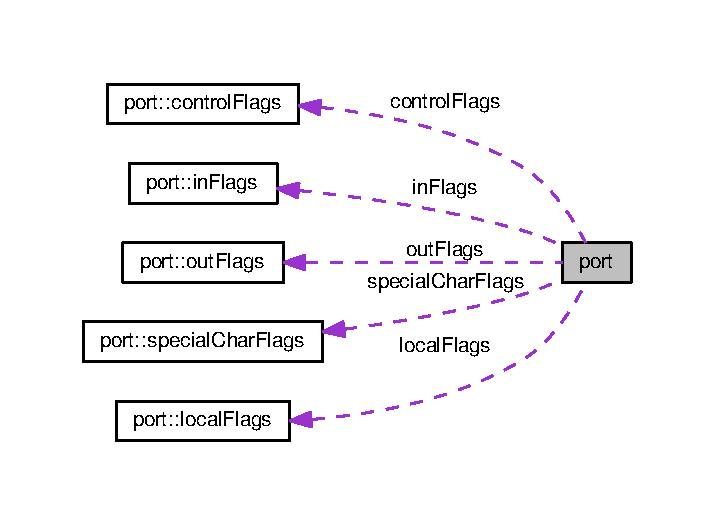
\includegraphics[width=343pt]{classport__coll__graph}
\end{center}
\end{figure}
\subsection*{Classes}
\begin{DoxyCompactItemize}
\item 
class \hyperlink{classport_1_1controlFlags}{control\+Flags}
\begin{DoxyCompactList}\small\item\em Class containing the statuses of termios.\+c\+\_\+cflag, constants for \mbox{[} C\+O\+N\+T\+R\+OL \mbox{]}. \end{DoxyCompactList}\item 
class \hyperlink{classport_1_1inFlags}{in\+Flags}
\begin{DoxyCompactList}\small\item\em Class containing the statuses of termios.\+c\+\_\+iflag, constants for \mbox{[} I\+N\+P\+UT \mbox{]}. \end{DoxyCompactList}\item 
class \hyperlink{classport_1_1localFlags}{local\+Flags}
\begin{DoxyCompactList}\small\item\em Class containing the statuses of termios.\+c\+\_\+lflag, constants for \mbox{[} L\+O\+C\+AL M\+O\+D\+ES \mbox{]}. \end{DoxyCompactList}\item 
class \hyperlink{classport_1_1outFlags}{out\+Flags}
\begin{DoxyCompactList}\small\item\em Class containing the statuses of termios.\+c\+\_\+oflag, constants for \mbox{[} O\+U\+T\+P\+UT \mbox{]}. \end{DoxyCompactList}\item 
class \hyperlink{classport_1_1specialCharFlags}{special\+Char\+Flags}
\end{DoxyCompactItemize}
\subsection*{Public Member Functions}
\begin{DoxyCompactItemize}
\item 
\hyperlink{classport_a5f40cbc450a8b0342a79b6e7ca4886e9}{port} ()
\item 
{\bfseries port} (std\+::string i\+Name, unsigned int i\+Baud)\hypertarget{classport_a1d2f8f629710d8f719d6641305d662f4}{}\label{classport_a1d2f8f629710d8f719d6641305d662f4}

\item 
\hyperlink{classport_acc336a1b8c9dacdd42914db803f2bd60}{port} (std\+::string i\+Name, unsigned int i\+Baud, unsigned char i\+Data\+Bits, unsigned char i\+Parity, unsigned char i\+Stop\+Bits)
\item 
\hyperlink{classport_a56b439f7dc620ddae93fa15bd8337cad}{port} (std\+::string i\+Name, unsigned int i\+Baud, unsigned char i\+Data\+Bits, std\+::string i\+Parity, std\+::string i\+Stop\+Bits)
\item 
void {\bfseries show\+\_\+all\+\_\+options} ()\hypertarget{classport_acaea3feacd669eac2f0c43c077727405}{}\label{classport_acaea3feacd669eac2f0c43c077727405}

\item 
void {\bfseries set\+Name} (std\+::string i\+Name)\hypertarget{classport_ab6ae1d0566a3e8df1d660892695f28ab}{}\label{classport_ab6ae1d0566a3e8df1d660892695f28ab}

\item 
std\+::string {\bfseries get\+Name} ()\hypertarget{classport_aaec0b4abf712f703fef9148e03cf9270}{}\label{classport_aaec0b4abf712f703fef9148e03cf9270}

\item 
void {\bfseries set\+Baud} (unsigned int i\+Baud)\hypertarget{classport_a305ee41a458ae38a0fa993b493be3563}{}\label{classport_a305ee41a458ae38a0fa993b493be3563}

\item 
unsigned int {\bfseries get\+Baud} ()\hypertarget{classport_a631542200faf4b6174f6b8ff46a0b1c0}{}\label{classport_a631542200faf4b6174f6b8ff46a0b1c0}

\item 
std\+::string {\bfseries get\+Baud\+\_\+\+Str} ()\hypertarget{classport_a5cdec26dd0ef22a9a529deed6bb15711}{}\label{classport_a5cdec26dd0ef22a9a529deed6bb15711}

\item 
void {\bfseries set\+Data\+Bits} (unsigned char i\+Data\+Bits)\hypertarget{classport_a27054cad9622e4ea62b6815de8058a90}{}\label{classport_a27054cad9622e4ea62b6815de8058a90}

\item 
unsigned char {\bfseries get\+Data\+Bits} ()\hypertarget{classport_a4653450ab48e69b23daedefdaf87082a}{}\label{classport_a4653450ab48e69b23daedefdaf87082a}

\item 
void {\bfseries set\+Parity} (unsigned char i\+Parity)\hypertarget{classport_a2e578abf2702fd3fea078fa9c8cf36b3}{}\label{classport_a2e578abf2702fd3fea078fa9c8cf36b3}

\item 
void {\bfseries set\+Parity} (std\+::string i\+Parity)\hypertarget{classport_ad190d97fa0661e762f40d552938c5fe4}{}\label{classport_ad190d97fa0661e762f40d552938c5fe4}

\item 
unsigned char {\bfseries get\+Parity} ()\hypertarget{classport_a6783f06829cc7007eeefa043a0a1883f}{}\label{classport_a6783f06829cc7007eeefa043a0a1883f}

\item 
std\+::string {\bfseries get\+Parity\+\_\+\+Str} ()\hypertarget{classport_a7c339a3de67e131387823837603b9534}{}\label{classport_a7c339a3de67e131387823837603b9534}

\item 
void {\bfseries set\+Stop\+Bits} (unsigned char i\+Stop\+Bits)\hypertarget{classport_a0241c8de6b2f9ce600ef343e94705b91}{}\label{classport_a0241c8de6b2f9ce600ef343e94705b91}

\item 
void {\bfseries set\+Stop\+Bits} (std\+::string i\+Stop\+Bits)\hypertarget{classport_afcffd414fdecf2847fbad056e34479d0}{}\label{classport_afcffd414fdecf2847fbad056e34479d0}

\item 
unsigned char {\bfseries get\+Stop\+Bits} ()\hypertarget{classport_a0329d9757f38df74f3984b97bb2c7815}{}\label{classport_a0329d9757f38df74f3984b97bb2c7815}

\item 
std\+::string {\bfseries get\+Stop\+Bits\+\_\+\+Str} ()\hypertarget{classport_a87617d86fb42ccb4d4c3de19372309dc}{}\label{classport_a87617d86fb42ccb4d4c3de19372309dc}

\item 
bool \hyperlink{classport_acd818c2e27262bc0d0e3312e3d318e4f}{do\+Open} ()
\item 
bool {\bfseries do\+Close} ()\hypertarget{classport_a3613644a1d121ccfdb4f208b9d85f89b}{}\label{classport_a3613644a1d121ccfdb4f208b9d85f89b}

\item 
int {\bfseries save\+Config} ()\hypertarget{classport_a63e4344186ebd989e5a44fdf444e74a9}{}\label{classport_a63e4344186ebd989e5a44fdf444e74a9}

\item 
int {\bfseries apply\+Config} ()\hypertarget{classport_aefbabdf3b06ca74528106a8fe722604b}{}\label{classport_aefbabdf3b06ca74528106a8fe722604b}

\item 
int {\bfseries restore\+Config} ()\hypertarget{classport_a1a31287c04e78a684975e9bec7c1488b}{}\label{classport_a1a31287c04e78a684975e9bec7c1488b}

\item 
\hyperlink{classserial__error}{serial\+\_\+error} $\ast$ {\bfseries get\+Error} ()\hypertarget{classport_a3b96e233b8d6818c05908cc52c4c1e97}{}\label{classport_a3b96e233b8d6818c05908cc52c4c1e97}

\item 
void \hyperlink{classport_a407a8f3980ae8d602e74cc4d783f000c}{set\+I\+G\+N\+B\+RK} (bool val)
\begin{DoxyCompactList}\small\item\em function void \hyperlink{classport_a407a8f3980ae8d602e74cc4d783f000c}{port\+::set\+I\+G\+N\+B\+RK} (bool val) \end{DoxyCompactList}\item 
bool \hyperlink{classport_a2118bd7b0b98bacf6d4b72c1811f04e3}{get\+I\+G\+N\+B\+RK} ()
\begin{DoxyCompactList}\small\item\em function bool \hyperlink{classport_a2118bd7b0b98bacf6d4b72c1811f04e3}{port\+::get\+I\+G\+N\+B\+RK} () \end{DoxyCompactList}\item 
void \hyperlink{classport_af71e9b2220f1cd1064c3f4071e05401c}{set\+B\+R\+K\+I\+NT} (bool val)
\begin{DoxyCompactList}\small\item\em function void \hyperlink{classport_af71e9b2220f1cd1064c3f4071e05401c}{port\+::set\+B\+R\+K\+I\+NT} (bool val) \end{DoxyCompactList}\item 
bool \hyperlink{classport_adb2359f5731d74ec463766f25842f4b0}{get\+B\+R\+K\+I\+NT} ()
\begin{DoxyCompactList}\small\item\em function bool \hyperlink{classport_adb2359f5731d74ec463766f25842f4b0}{port\+::get\+B\+R\+K\+I\+NT} () \end{DoxyCompactList}\item 
void \hyperlink{classport_ae669f4e4d581ea011e42ddd2f550f8d7}{set\+I\+G\+N\+P\+AR} (bool val)
\begin{DoxyCompactList}\small\item\em function void \hyperlink{classport_ae669f4e4d581ea011e42ddd2f550f8d7}{port\+::set\+I\+G\+N\+P\+AR} (bool val) \end{DoxyCompactList}\item 
bool \hyperlink{classport_af76be254c1c7bbb23a082dd16868a2d9}{get\+I\+G\+N\+P\+AR} ()
\begin{DoxyCompactList}\small\item\em function bool \hyperlink{classport_af76be254c1c7bbb23a082dd16868a2d9}{port\+::get\+I\+G\+N\+P\+AR} () \end{DoxyCompactList}\item 
void \hyperlink{classport_a82283d6d16531d32b6a41e00b81b6c02}{set\+P\+A\+R\+M\+RK} (bool val)
\begin{DoxyCompactList}\small\item\em function void \hyperlink{classport_a82283d6d16531d32b6a41e00b81b6c02}{port\+::set\+P\+A\+R\+M\+RK} (bool val) \end{DoxyCompactList}\item 
bool \hyperlink{classport_a92d004da4e55ba28f1bef98a92a3db29}{get\+P\+A\+R\+M\+RK} ()
\begin{DoxyCompactList}\small\item\em function bool \hyperlink{classport_a92d004da4e55ba28f1bef98a92a3db29}{port\+::get\+P\+A\+R\+M\+RK} () \end{DoxyCompactList}\item 
void \hyperlink{classport_ad021eae5176782417807c3788ae2235e}{set\+I\+N\+P\+CK} (bool val)
\begin{DoxyCompactList}\small\item\em function void \hyperlink{classport_ad021eae5176782417807c3788ae2235e}{port\+::set\+I\+N\+P\+CK} (bool val) \end{DoxyCompactList}\item 
bool \hyperlink{classport_a4699e4d4d41fbafc84283aec74033332}{get\+I\+N\+P\+CK} ()
\begin{DoxyCompactList}\small\item\em function bool \hyperlink{classport_a4699e4d4d41fbafc84283aec74033332}{port\+::get\+I\+N\+P\+CK} () \end{DoxyCompactList}\item 
void \hyperlink{classport_ab9f983c471a53c5646d45038a4336302}{set\+I\+S\+T\+R\+IP} (bool val)
\begin{DoxyCompactList}\small\item\em function void \hyperlink{classport_ab9f983c471a53c5646d45038a4336302}{port\+::set\+I\+S\+T\+R\+IP} (bool val) \end{DoxyCompactList}\item 
bool \hyperlink{classport_a0dc8e00aedf6ddc490addefd1a780f54}{get\+I\+S\+T\+R\+IP} ()
\begin{DoxyCompactList}\small\item\em function bool \hyperlink{classport_a0dc8e00aedf6ddc490addefd1a780f54}{port\+::get\+I\+S\+T\+R\+IP} () \end{DoxyCompactList}\item 
void \hyperlink{classport_a548740957c8a76fbc143b000a999539c}{set\+I\+N\+L\+CR} (bool val)
\begin{DoxyCompactList}\small\item\em function void \hyperlink{classport_a548740957c8a76fbc143b000a999539c}{port\+::set\+I\+N\+L\+CR} (bool val) \end{DoxyCompactList}\item 
bool \hyperlink{classport_a263aa63cc21b4966106d954a4bea63fa}{get\+I\+N\+L\+CR} ()
\begin{DoxyCompactList}\small\item\em function bool \hyperlink{classport_a263aa63cc21b4966106d954a4bea63fa}{port\+::get\+I\+N\+L\+CR} () \end{DoxyCompactList}\item 
void \hyperlink{classport_ad79cac75e27d960cabe7a06572b7b1a0}{set\+I\+G\+N\+CR} (bool val)
\begin{DoxyCompactList}\small\item\em function void \hyperlink{classport_ad79cac75e27d960cabe7a06572b7b1a0}{port\+::set\+I\+G\+N\+CR} (bool val) \end{DoxyCompactList}\item 
bool \hyperlink{classport_a9c489a19354c6d711755d54664d2f701}{get\+I\+G\+N\+CR} ()
\begin{DoxyCompactList}\small\item\em function bool \hyperlink{classport_a9c489a19354c6d711755d54664d2f701}{port\+::get\+I\+G\+N\+CR} () \end{DoxyCompactList}\item 
void \hyperlink{classport_a5087059119c84da88e99145604a8ebf5}{set\+I\+C\+R\+NL} (bool val)
\begin{DoxyCompactList}\small\item\em function void \hyperlink{classport_a5087059119c84da88e99145604a8ebf5}{port\+::set\+I\+C\+R\+NL} (bool val) \end{DoxyCompactList}\item 
bool \hyperlink{classport_a3024c478a8a7f754e5eb2b50ff733b81}{get\+I\+C\+R\+NL} ()
\begin{DoxyCompactList}\small\item\em function bool \hyperlink{classport_a3024c478a8a7f754e5eb2b50ff733b81}{port\+::get\+I\+C\+R\+NL} () \end{DoxyCompactList}\item 
void \hyperlink{classport_a05f341eef4091a50c0fdb6742ba5e9cf}{set\+I\+X\+ON} (bool val)
\begin{DoxyCompactList}\small\item\em function void \hyperlink{classport_a05f341eef4091a50c0fdb6742ba5e9cf}{port\+::set\+I\+X\+ON} (bool val) \end{DoxyCompactList}\item 
bool \hyperlink{classport_ab57c3459ef2ee5d76b6e996f46b66bcc}{get\+I\+X\+ON} ()
\begin{DoxyCompactList}\small\item\em function bool \hyperlink{classport_ab57c3459ef2ee5d76b6e996f46b66bcc}{port\+::get\+I\+X\+ON} () \end{DoxyCompactList}\item 
void \hyperlink{classport_a0598bc43a59cb71fb08060249d7805da}{set\+I\+X\+O\+FF} (bool val)
\begin{DoxyCompactList}\small\item\em function void \hyperlink{classport_a0598bc43a59cb71fb08060249d7805da}{port\+::set\+I\+X\+O\+FF} (bool val) \end{DoxyCompactList}\item 
bool \hyperlink{classport_a3d517d3f06731348488002fea13b8e88}{get\+I\+X\+O\+FF} ()
\begin{DoxyCompactList}\small\item\em function bool \hyperlink{classport_a3d517d3f06731348488002fea13b8e88}{port\+::get\+I\+X\+O\+FF} () \end{DoxyCompactList}\item 
void \hyperlink{classport_afa286d567530f7b124b7fc2caac4d61a}{set\+I\+X\+A\+NY} (bool val)
\begin{DoxyCompactList}\small\item\em function void \hyperlink{classport_afa286d567530f7b124b7fc2caac4d61a}{port\+::set\+I\+X\+A\+NY} (bool val) \end{DoxyCompactList}\item 
bool \hyperlink{classport_a4a85ca57362115255b5e0049b90ff4e7}{get\+I\+X\+A\+NY} ()
\begin{DoxyCompactList}\small\item\em function bool \hyperlink{classport_a4a85ca57362115255b5e0049b90ff4e7}{port\+::get\+I\+X\+A\+NY} () \end{DoxyCompactList}\item 
void \hyperlink{classport_a7e2ce41de280c0167bcf414c2cbe5dcf}{set\+I\+U\+T\+F8} (bool val)
\begin{DoxyCompactList}\small\item\em function void \hyperlink{classport_a7e2ce41de280c0167bcf414c2cbe5dcf}{port\+::set\+I\+U\+T\+F8} (bool val) \end{DoxyCompactList}\item 
bool \hyperlink{classport_a9575ab3023169a91c984f458702c2f53}{get\+I\+U\+T\+F8} ()
\begin{DoxyCompactList}\small\item\em function bool \hyperlink{classport_a9575ab3023169a91c984f458702c2f53}{port\+::get\+I\+U\+T\+F8} () \end{DoxyCompactList}\item 
void \hyperlink{classport_a4c7b692b00a8a85b4155e672a8673117}{set\+O\+P\+O\+ST} (bool val)
\begin{DoxyCompactList}\small\item\em function void \hyperlink{classport_a4c7b692b00a8a85b4155e672a8673117}{port\+::set\+O\+P\+O\+ST} (bool val) \end{DoxyCompactList}\item 
bool \hyperlink{classport_a622d4dabe322c92f2721d0fdaa35d583}{get\+O\+P\+O\+ST} ()
\begin{DoxyCompactList}\small\item\em function bool \hyperlink{classport_a622d4dabe322c92f2721d0fdaa35d583}{port\+::get\+O\+P\+O\+ST} () \end{DoxyCompactList}\item 
void \hyperlink{classport_aa44c9d03000e78c1797fcc02023e0a30}{set\+O\+N\+L\+CR} (bool val)
\begin{DoxyCompactList}\small\item\em function void \hyperlink{classport_aa44c9d03000e78c1797fcc02023e0a30}{port\+::set\+O\+N\+L\+CR} (bool val) \end{DoxyCompactList}\item 
bool \hyperlink{classport_a5c5529b9412799359a9a063d8694baa1}{get\+O\+N\+L\+CR} ()
\begin{DoxyCompactList}\small\item\em function bool \hyperlink{classport_a5c5529b9412799359a9a063d8694baa1}{port\+::get\+O\+N\+L\+CR} () \end{DoxyCompactList}\item 
void \hyperlink{classport_af9ff8713572bcacfd765f13d6dcb8a61}{set\+O\+C\+R\+NL} (bool val)
\begin{DoxyCompactList}\small\item\em function void \hyperlink{classport_af9ff8713572bcacfd765f13d6dcb8a61}{port\+::set\+O\+C\+R\+NL} (bool val) \end{DoxyCompactList}\item 
bool \hyperlink{classport_aac6ca3065f7bb33386af3a9e0ed0a0a1}{get\+O\+C\+R\+NL} ()
\begin{DoxyCompactList}\small\item\em function bool \hyperlink{classport_aac6ca3065f7bb33386af3a9e0ed0a0a1}{port\+::get\+O\+C\+R\+NL} () \end{DoxyCompactList}\item 
void \hyperlink{classport_a68f1dc6b5d1250c2c6a3bc4e1f435b1b}{set\+O\+N\+O\+CR} (bool val)
\begin{DoxyCompactList}\small\item\em function void \hyperlink{classport_a68f1dc6b5d1250c2c6a3bc4e1f435b1b}{port\+::set\+O\+N\+O\+CR} (bool val) \end{DoxyCompactList}\item 
bool \hyperlink{classport_a2a7a1ac23b994b559dc45c6c1e20c46b}{get\+O\+N\+O\+CR} ()
\begin{DoxyCompactList}\small\item\em function bool \hyperlink{classport_a2a7a1ac23b994b559dc45c6c1e20c46b}{port\+::get\+O\+N\+O\+CR} () \end{DoxyCompactList}\item 
void \hyperlink{classport_ad68aa35b00421eb9a30e246bdbb8ddb8}{set\+O\+N\+L\+R\+ET} (bool val)
\begin{DoxyCompactList}\small\item\em function void \hyperlink{classport_ad68aa35b00421eb9a30e246bdbb8ddb8}{port\+::set\+O\+N\+L\+R\+ET} (bool val) \end{DoxyCompactList}\item 
bool \hyperlink{classport_a4c5aa09daf221a9409e91b279da17669}{get\+O\+N\+L\+R\+ET} ()
\begin{DoxyCompactList}\small\item\em function bool \hyperlink{classport_a4c5aa09daf221a9409e91b279da17669}{port\+::get\+O\+N\+L\+R\+ET} () \end{DoxyCompactList}\item 
void \hyperlink{classport_a38f6eec5e22daede6d707d6ca4a29784}{set\+O\+F\+I\+LL} (bool val)
\begin{DoxyCompactList}\small\item\em function void \hyperlink{classport_a38f6eec5e22daede6d707d6ca4a29784}{port\+::set\+O\+F\+I\+LL} (bool val) \end{DoxyCompactList}\item 
bool \hyperlink{classport_a087e732d81656583ce7430727263149a}{get\+O\+F\+I\+LL} ()
\begin{DoxyCompactList}\small\item\em function bool \hyperlink{classport_a087e732d81656583ce7430727263149a}{port\+::get\+O\+F\+I\+LL} () \end{DoxyCompactList}\item 
int \hyperlink{classport_a2a2bc570ded985a9f5a7807974a955ba}{set\+N\+L\+D\+LY} (std\+::string in\+Str)
\begin{DoxyCompactList}\small\item\em function int \hyperlink{classport_a2a2bc570ded985a9f5a7807974a955ba}{port\+::set\+N\+L\+D\+LY} (std\+::string in\+Str) \end{DoxyCompactList}\item 
std\+::string \hyperlink{classport_aae2ce70c879b30f001563968a1ef5a34}{get\+N\+L\+D\+LY} ()
\begin{DoxyCompactList}\small\item\em function std\+::string \hyperlink{classport_aae2ce70c879b30f001563968a1ef5a34}{port\+::get\+N\+L\+D\+LY} () \end{DoxyCompactList}\item 
int \hyperlink{classport_afca1f60b0977cd228f12a8ef4c771fc4}{set\+C\+R\+D\+LY} (std\+::string in\+Str)
\begin{DoxyCompactList}\small\item\em function int \hyperlink{classport_afca1f60b0977cd228f12a8ef4c771fc4}{port\+::set\+C\+R\+D\+LY} (std\+::string in\+Str) \end{DoxyCompactList}\item 
std\+::string \hyperlink{classport_a4977770fd7700ed83c1aeb290de881a3}{get\+C\+R\+D\+LY} ()
\begin{DoxyCompactList}\small\item\em function std\+::string \hyperlink{classport_a4977770fd7700ed83c1aeb290de881a3}{port\+::get\+C\+R\+D\+LY} () \end{DoxyCompactList}\item 
int \hyperlink{classport_a67bc0162f685499eed5d57e4be9d9272}{set\+T\+A\+B\+D\+LY} (std\+::string in\+Str)
\begin{DoxyCompactList}\small\item\em function int \hyperlink{classport_a67bc0162f685499eed5d57e4be9d9272}{port\+::set\+T\+A\+B\+D\+LY} (string in\+Str) \end{DoxyCompactList}\item 
std\+::string \hyperlink{classport_a481eb9d22358475a06bacd5368e6fb28}{get\+T\+A\+B\+D\+LY} ()
\begin{DoxyCompactList}\small\item\em function std\+::string \hyperlink{classport_a481eb9d22358475a06bacd5368e6fb28}{port\+::get\+T\+A\+B\+D\+LY} () \end{DoxyCompactList}\item 
int \hyperlink{classport_a659fafa1c6894eeb8d850868b79141e6}{set\+V\+T\+D\+LY} (std\+::string in\+Str)
\begin{DoxyCompactList}\small\item\em function int \hyperlink{classport_a659fafa1c6894eeb8d850868b79141e6}{port\+::set\+V\+T\+D\+LY} (string in\+Str) \end{DoxyCompactList}\item 
std\+::string \hyperlink{classport_a7f0a523dd9a9db4549788da5c79cf846}{get\+V\+T\+D\+LY} ()
\begin{DoxyCompactList}\small\item\em function std\+::string \hyperlink{classport_a7f0a523dd9a9db4549788da5c79cf846}{port\+::get\+V\+T\+D\+LY} () \end{DoxyCompactList}\item 
int \hyperlink{classport_aac53f4a9f4f82a6886d7d3ea3a313880}{set\+F\+F\+D\+LY} (std\+::string in\+Str)
\begin{DoxyCompactList}\small\item\em function int \hyperlink{classport_aac53f4a9f4f82a6886d7d3ea3a313880}{port\+::set\+F\+F\+D\+LY} (string in\+Str) \end{DoxyCompactList}\item 
std\+::string \hyperlink{classport_a5f6dee4481213d1b9af115b379a872b4}{get\+F\+F\+D\+LY} ()
\begin{DoxyCompactList}\small\item\em function std\+::string \hyperlink{classport_a5f6dee4481213d1b9af115b379a872b4}{port\+::get\+F\+F\+D\+LY} () \end{DoxyCompactList}\item 
int \hyperlink{classport_a4a5196aff46a1bbd7d83d451fb0a1f84}{set\+C\+S\+I\+ZE} (std\+::string in\+Str)
\begin{DoxyCompactList}\small\item\em function int \hyperlink{classport_a4a5196aff46a1bbd7d83d451fb0a1f84}{port\+::set\+C\+S\+I\+ZE} (string in\+Str) \end{DoxyCompactList}\item 
std\+::string \hyperlink{classport_ae522c4cf7e2eb5e89d3b062ad1a6270e}{get\+C\+S\+I\+ZE} ()
\begin{DoxyCompactList}\small\item\em function std\+::string \hyperlink{classport_ae522c4cf7e2eb5e89d3b062ad1a6270e}{port\+::get\+C\+S\+I\+ZE} () \end{DoxyCompactList}\item 
void \hyperlink{classport_ac118b2b26d60ffe58e11f7b6c75c8260}{set\+C\+S\+T\+O\+PB} (bool val)
\begin{DoxyCompactList}\small\item\em function void \hyperlink{classport_ac118b2b26d60ffe58e11f7b6c75c8260}{port\+::set\+C\+S\+T\+O\+PB} (bool val) \end{DoxyCompactList}\item 
bool \hyperlink{classport_ac792060b6fc53cea0e0a3476b338ddb3}{get\+C\+S\+T\+O\+PB} ()
\begin{DoxyCompactList}\small\item\em function bool \hyperlink{classport_ac792060b6fc53cea0e0a3476b338ddb3}{port\+::get\+C\+S\+T\+O\+PB} () \end{DoxyCompactList}\item 
void \hyperlink{classport_ade51ac47a0f6247189d7fcf143ac2246}{set\+C\+R\+E\+AD} (bool val)
\begin{DoxyCompactList}\small\item\em function void \hyperlink{classport_ade51ac47a0f6247189d7fcf143ac2246}{port\+::set\+C\+R\+E\+AD} (bool val) \end{DoxyCompactList}\item 
bool \hyperlink{classport_a8c686ab18882de329b1c5666688724d6}{get\+C\+R\+E\+AD} ()
\begin{DoxyCompactList}\small\item\em function bool \hyperlink{classport_a8c686ab18882de329b1c5666688724d6}{port\+::get\+C\+R\+E\+AD} () \end{DoxyCompactList}\item 
void \hyperlink{classport_a38427fe381f2db5d296748d426ca58bf}{set\+P\+A\+R\+E\+NB} (bool val)
\begin{DoxyCompactList}\small\item\em function void \hyperlink{classport_a38427fe381f2db5d296748d426ca58bf}{port\+::set\+P\+A\+R\+E\+NB} (bool val) \end{DoxyCompactList}\item 
bool \hyperlink{classport_a4d3e68b6545fdfae4b62d94c152aa5c5}{get\+P\+A\+R\+E\+NB} ()
\begin{DoxyCompactList}\small\item\em function bool \hyperlink{classport_a4d3e68b6545fdfae4b62d94c152aa5c5}{port\+::get\+P\+A\+R\+E\+NB} () \end{DoxyCompactList}\item 
void \hyperlink{classport_ac236d1a60de223b09b225708c11d3c95}{set\+P\+A\+R\+O\+DD} (bool val)
\begin{DoxyCompactList}\small\item\em function void \hyperlink{classport_ac236d1a60de223b09b225708c11d3c95}{port\+::set\+P\+A\+R\+O\+DD} (bool val) \end{DoxyCompactList}\item 
bool \hyperlink{classport_ac07219c7d113a9671c8b00e3e6e9e26a}{get\+P\+A\+R\+O\+DD} ()
\begin{DoxyCompactList}\small\item\em function bool \hyperlink{classport_ac07219c7d113a9671c8b00e3e6e9e26a}{port\+::get\+P\+A\+R\+O\+DD} () \end{DoxyCompactList}\item 
void \hyperlink{classport_aebb52d4483ac46fc85b44f5839a56f10}{set\+H\+U\+P\+CL} (bool val)
\begin{DoxyCompactList}\small\item\em function void \hyperlink{classport_aebb52d4483ac46fc85b44f5839a56f10}{port\+::set\+H\+U\+P\+CL} (bool val) \end{DoxyCompactList}\item 
bool \hyperlink{classport_a6d49ff5c1b9d5dd932c08986e261f090}{get\+H\+U\+P\+CL} ()
\begin{DoxyCompactList}\small\item\em function bool \hyperlink{classport_a6d49ff5c1b9d5dd932c08986e261f090}{port\+::get\+H\+U\+P\+CL} () \end{DoxyCompactList}\item 
void \hyperlink{classport_a4a9d4fc5915b00350438f5e7319fb23e}{set\+C\+L\+O\+C\+AL} (bool val)
\begin{DoxyCompactList}\small\item\em function void \hyperlink{classport_a4a9d4fc5915b00350438f5e7319fb23e}{port\+::set\+C\+L\+O\+C\+AL} (bool val) \end{DoxyCompactList}\item 
bool \hyperlink{classport_a623de59915a0b9dd51ed6045828c4a1c}{get\+C\+L\+O\+C\+AL} ()
\begin{DoxyCompactList}\small\item\em function bool \hyperlink{classport_a623de59915a0b9dd51ed6045828c4a1c}{port\+::get\+C\+L\+O\+C\+AL} () \end{DoxyCompactList}\item 
void \hyperlink{classport_a5e1a90cfde8ddb3240e0f6f12e0ebe80}{set\+I\+S\+IG} (bool val)
\begin{DoxyCompactList}\small\item\em function void \hyperlink{classport_a5e1a90cfde8ddb3240e0f6f12e0ebe80}{port\+::set\+I\+S\+IG} (bool val) \end{DoxyCompactList}\item 
bool \hyperlink{classport_a4d394ecfaebb015a16a93ebca7afea22}{get\+I\+S\+IG} ()
\begin{DoxyCompactList}\small\item\em function bool \hyperlink{classport_a4d394ecfaebb015a16a93ebca7afea22}{port\+::get\+I\+S\+IG} () \end{DoxyCompactList}\item 
void \hyperlink{classport_a2975fb4424cccd46e2da267bd53e3ad0}{set\+I\+C\+A\+N\+ON} (bool val)
\begin{DoxyCompactList}\small\item\em function void \hyperlink{classport_a2975fb4424cccd46e2da267bd53e3ad0}{port\+::set\+I\+C\+A\+N\+ON} (bool val) \end{DoxyCompactList}\item 
bool \hyperlink{classport_a50945a4a78dd74a71004878d38c7cc97}{get\+I\+C\+A\+N\+ON} ()
\begin{DoxyCompactList}\small\item\em function bool \hyperlink{classport_a50945a4a78dd74a71004878d38c7cc97}{port\+::get\+I\+C\+A\+N\+ON} () \end{DoxyCompactList}\item 
void \hyperlink{classport_ab00aa47d139c536a84ca0b2ec9f8ef96}{set\+E\+C\+HO} (bool val)
\begin{DoxyCompactList}\small\item\em function void \hyperlink{classport_ab00aa47d139c536a84ca0b2ec9f8ef96}{port\+::set\+E\+C\+HO} (bool val) \end{DoxyCompactList}\item 
bool \hyperlink{classport_af6aaa84a4759991f80963c457530e151}{get\+E\+C\+HO} ()
\begin{DoxyCompactList}\small\item\em function bool \hyperlink{classport_af6aaa84a4759991f80963c457530e151}{port\+::get\+E\+C\+HO} () \end{DoxyCompactList}\item 
void \hyperlink{classport_a0ae016ddf513a4dec27e7fb4e91a45a1}{set\+E\+C\+H\+OE} (bool val)
\begin{DoxyCompactList}\small\item\em function void \hyperlink{classport_a0ae016ddf513a4dec27e7fb4e91a45a1}{port\+::set\+E\+C\+H\+OE} (bool val) \end{DoxyCompactList}\item 
bool \hyperlink{classport_a54f8ecafc33c840d4d4a7bd928968916}{get\+E\+C\+H\+OE} ()
\begin{DoxyCompactList}\small\item\em function bool \hyperlink{classport_a54f8ecafc33c840d4d4a7bd928968916}{port\+::get\+E\+C\+H\+OE} () \end{DoxyCompactList}\item 
void \hyperlink{classport_abf70fa210c1c01f08868526c908042fd}{set\+E\+C\+H\+OK} (bool val)
\begin{DoxyCompactList}\small\item\em function void \hyperlink{classport_abf70fa210c1c01f08868526c908042fd}{port\+::set\+E\+C\+H\+OK} (bool val) \end{DoxyCompactList}\item 
bool \hyperlink{classport_af358e760f826378bdbff0c338b3561aa}{get\+E\+C\+H\+OK} ()
\begin{DoxyCompactList}\small\item\em function bool \hyperlink{classport_af358e760f826378bdbff0c338b3561aa}{port\+::get\+E\+C\+H\+OK} () \end{DoxyCompactList}\item 
void \hyperlink{classport_a96a45d5c9d0e6c3546be94a8477a03d9}{set\+E\+C\+H\+O\+NL} (bool val)
\begin{DoxyCompactList}\small\item\em function void \hyperlink{classport_abf70fa210c1c01f08868526c908042fd}{port\+::set\+E\+C\+H\+OK} (bool val) \end{DoxyCompactList}\item 
bool \hyperlink{classport_a0ed3a5bcfe7dc3f3d0425ccda06d68a3}{get\+E\+C\+H\+O\+NL} ()
\begin{DoxyCompactList}\small\item\em function bool \hyperlink{classport_a0ed3a5bcfe7dc3f3d0425ccda06d68a3}{port\+::get\+E\+C\+H\+O\+NL} () \end{DoxyCompactList}\item 
void \hyperlink{classport_a5676edc2cd36b51b79987f01ca0159c9}{set\+N\+O\+F\+L\+SH} (bool val)
\begin{DoxyCompactList}\small\item\em function void \hyperlink{classport_a5676edc2cd36b51b79987f01ca0159c9}{port\+::set\+N\+O\+F\+L\+SH} (bool val) \end{DoxyCompactList}\item 
bool \hyperlink{classport_a90648b5c129f002697c88312d43404b5}{get\+N\+O\+F\+L\+SH} ()
\begin{DoxyCompactList}\small\item\em function bool \hyperlink{classport_a90648b5c129f002697c88312d43404b5}{port\+::get\+N\+O\+F\+L\+SH} () \end{DoxyCompactList}\item 
void \hyperlink{classport_a850aef33a8b6060e55b19dfee565bcc6}{set\+T\+O\+S\+T\+OP} (bool val)
\begin{DoxyCompactList}\small\item\em function void \hyperlink{classport_a850aef33a8b6060e55b19dfee565bcc6}{port\+::set\+T\+O\+S\+T\+OP} (bool val) \end{DoxyCompactList}\item 
bool \hyperlink{classport_a8c22333e40cecf5d0c9a21f11ab94b57}{get\+T\+O\+S\+T\+OP} ()
\begin{DoxyCompactList}\small\item\em function bool \hyperlink{classport_a8c22333e40cecf5d0c9a21f11ab94b57}{port\+::get\+T\+O\+S\+T\+OP} () \end{DoxyCompactList}\item 
void \hyperlink{classport_aee20c776c3696976fd00203343441e1b}{set\+I\+E\+X\+T\+EN} (bool val)
\begin{DoxyCompactList}\small\item\em function void \hyperlink{classport_aee20c776c3696976fd00203343441e1b}{port\+::set\+I\+E\+X\+T\+EN} (bool val) \end{DoxyCompactList}\item 
bool \hyperlink{classport_a513d3fa647f662f93467da579ae510e8}{get\+I\+E\+X\+T\+EN} ()
\begin{DoxyCompactList}\small\item\em function bool \hyperlink{classport_a513d3fa647f662f93467da579ae510e8}{port\+::get\+I\+E\+X\+T\+EN} () \end{DoxyCompactList}\item 
void \hyperlink{classport_a84c056e9f04f4fd3dc4200f6ba7279de}{set\+V\+E\+OF} (bool val)
\begin{DoxyCompactList}\small\item\em function void \hyperlink{classport_a84c056e9f04f4fd3dc4200f6ba7279de}{port\+::set\+V\+E\+OF} (bool val) \end{DoxyCompactList}\item 
bool \hyperlink{classport_a3dedfb7fd7aaeda7b85bcaaf40c1edc9}{get\+V\+E\+OF} ()
\begin{DoxyCompactList}\small\item\em function bool \hyperlink{classport_a3dedfb7fd7aaeda7b85bcaaf40c1edc9}{port\+::get\+V\+E\+OF} () \end{DoxyCompactList}\item 
void \hyperlink{classport_a99880c2c00863369ea5fa2e3fdfe8474}{set\+V\+E\+OL} (bool val)
\begin{DoxyCompactList}\small\item\em function void \hyperlink{classport_a99880c2c00863369ea5fa2e3fdfe8474}{port\+::set\+V\+E\+OL} (bool val) \end{DoxyCompactList}\item 
bool \hyperlink{classport_a381910916d501b1fde29803731dde7a5}{get\+V\+E\+OL} ()
\begin{DoxyCompactList}\small\item\em function bool \hyperlink{classport_a381910916d501b1fde29803731dde7a5}{port\+::get\+V\+E\+OL} () \end{DoxyCompactList}\item 
void \hyperlink{classport_abadd59db8333dd9793c267e55175a4fd}{set\+V\+E\+R\+A\+SE} (bool val)
\begin{DoxyCompactList}\small\item\em function void \hyperlink{classport_abadd59db8333dd9793c267e55175a4fd}{port\+::set\+V\+E\+R\+A\+SE} (bool val) \end{DoxyCompactList}\item 
bool \hyperlink{classport_a1e814b6f4a98d69126ceb79cc8c89e72}{get\+V\+E\+R\+A\+SE} ()
\begin{DoxyCompactList}\small\item\em function bool \hyperlink{classport_a1e814b6f4a98d69126ceb79cc8c89e72}{port\+::get\+V\+E\+R\+A\+SE} () \end{DoxyCompactList}\item 
void \hyperlink{classport_a3b11cfb6cb43b30329c811aca60e935f}{set\+V\+I\+N\+TR} (bool val)
\begin{DoxyCompactList}\small\item\em function void \hyperlink{classport_a3b11cfb6cb43b30329c811aca60e935f}{port\+::set\+V\+I\+N\+TR} (bool val) \end{DoxyCompactList}\item 
bool \hyperlink{classport_a7e274f5ddc4db2e0e613f10e14022a56}{get\+V\+I\+N\+TR} ()
\begin{DoxyCompactList}\small\item\em function bool \hyperlink{classport_a7e274f5ddc4db2e0e613f10e14022a56}{port\+::get\+V\+I\+N\+TR} () \end{DoxyCompactList}\item 
void \hyperlink{classport_a98b0148cac1cc3d9c7c0ae4b6224bcd5}{set\+V\+K\+I\+LL} (bool val)
\begin{DoxyCompactList}\small\item\em function void \hyperlink{classport_a98b0148cac1cc3d9c7c0ae4b6224bcd5}{port\+::set\+V\+K\+I\+LL} (bool val) \end{DoxyCompactList}\item 
bool \hyperlink{classport_a3d0ee5aefacdf3a0603415279c8b1f2e}{get\+V\+K\+I\+LL} ()
\begin{DoxyCompactList}\small\item\em function bool \hyperlink{classport_a3d0ee5aefacdf3a0603415279c8b1f2e}{port\+::get\+V\+K\+I\+LL} () \end{DoxyCompactList}\item 
void \hyperlink{classport_a4540b03345ee1d14fcc66e4f497ee53a}{set\+V\+M\+IN} (bool val)
\begin{DoxyCompactList}\small\item\em function void \hyperlink{classport_a4540b03345ee1d14fcc66e4f497ee53a}{port\+::set\+V\+M\+IN} (bool val) \end{DoxyCompactList}\item 
bool \hyperlink{classport_ada55fc3ad061d8ba22c43431033c99c2}{get\+V\+M\+IN} ()
\begin{DoxyCompactList}\small\item\em function bool \hyperlink{classport_ada55fc3ad061d8ba22c43431033c99c2}{port\+::get\+V\+M\+IN} () \end{DoxyCompactList}\item 
void \hyperlink{classport_ad1f7146621d17e698fdf3ae9e351638a}{set\+V\+Q\+U\+IT} (bool val)
\begin{DoxyCompactList}\small\item\em function void \hyperlink{classport_ad1f7146621d17e698fdf3ae9e351638a}{port\+::set\+V\+Q\+U\+IT} (bool val) \end{DoxyCompactList}\item 
bool \hyperlink{classport_abd1ce4d2e9195cce6c34b09d08bc17a1}{get\+V\+Q\+U\+IT} ()
\begin{DoxyCompactList}\small\item\em function bool \hyperlink{classport_abd1ce4d2e9195cce6c34b09d08bc17a1}{port\+::get\+V\+Q\+U\+IT} () \end{DoxyCompactList}\item 
void \hyperlink{classport_a54adef359503c44101291e34465c96cb}{set\+V\+S\+T\+A\+RT} (bool val)
\begin{DoxyCompactList}\small\item\em function void \hyperlink{classport_a54adef359503c44101291e34465c96cb}{port\+::set\+V\+S\+T\+A\+RT} (bool val) \end{DoxyCompactList}\item 
bool \hyperlink{classport_a6a3391f362c5da90f1a1d21128de0ed3}{get\+V\+S\+T\+A\+RT} ()
\begin{DoxyCompactList}\small\item\em function bool \hyperlink{classport_a6a3391f362c5da90f1a1d21128de0ed3}{port\+::get\+V\+S\+T\+A\+RT} () \end{DoxyCompactList}\item 
void \hyperlink{classport_ae7956d6922fca348e91bcf3838b9ef64}{set\+V\+S\+T\+OP} (bool val)
\begin{DoxyCompactList}\small\item\em function void \hyperlink{classport_ae7956d6922fca348e91bcf3838b9ef64}{port\+::set\+V\+S\+T\+OP} (bool val) \end{DoxyCompactList}\item 
bool \hyperlink{classport_a7f2941a597bee2be6d1baef10b086593}{get\+V\+S\+T\+OP} ()
\begin{DoxyCompactList}\small\item\em function bool \hyperlink{classport_a7f2941a597bee2be6d1baef10b086593}{port\+::get\+V\+S\+T\+OP} () \end{DoxyCompactList}\item 
void \hyperlink{classport_a4edaec529df920f3b0999e484657e402}{set\+V\+S\+U\+SP} (bool val)
\begin{DoxyCompactList}\small\item\em function void \hyperlink{classport_a4edaec529df920f3b0999e484657e402}{port\+::set\+V\+S\+U\+SP} (bool val) \end{DoxyCompactList}\item 
bool \hyperlink{classport_a7b5ae199c4b371da78674ce9cdba7f01}{get\+V\+S\+U\+SP} ()
\begin{DoxyCompactList}\small\item\em function bool \hyperlink{classport_a7b5ae199c4b371da78674ce9cdba7f01}{port\+::get\+V\+S\+U\+SP} () \end{DoxyCompactList}\item 
void \hyperlink{classport_a43d05a6b037dccbf2666b87d4b49313a}{set\+V\+T\+I\+ME} (unsigned int val)
\begin{DoxyCompactList}\small\item\em function void \hyperlink{classport_a43d05a6b037dccbf2666b87d4b49313a}{port\+::set\+V\+T\+I\+ME} (unsigned int val) \end{DoxyCompactList}\item 
unsigned int \hyperlink{classport_a0d929e2f0e5333b56cffb534c5f6fbdc}{get\+V\+T\+I\+ME} ()
\begin{DoxyCompactList}\small\item\em function unsigned int \hyperlink{classport_a0d929e2f0e5333b56cffb534c5f6fbdc}{port\+::get\+V\+T\+I\+ME} () \end{DoxyCompactList}\end{DoxyCompactItemize}
\subsection*{Public Attributes}
\begin{DoxyCompactItemize}
\item 
class \hyperlink{classport_1_1inFlags}{port\+::in\+Flags} {\bfseries in\+Flags}\hypertarget{classport_af0a59d590b28a89ce407b35a5b35e732}{}\label{classport_af0a59d590b28a89ce407b35a5b35e732}

\item 
class \hyperlink{classport_1_1outFlags}{port\+::out\+Flags} {\bfseries out\+Flags}\hypertarget{classport_a68b4c1db043259c0c329513990e8a9fc}{}\label{classport_a68b4c1db043259c0c329513990e8a9fc}

\item 
class \hyperlink{classport_1_1controlFlags}{port\+::control\+Flags} {\bfseries control\+Flags}\hypertarget{classport_a0a1349f99d686112de07ba7d3ddc3c0c}{}\label{classport_a0a1349f99d686112de07ba7d3ddc3c0c}

\item 
class \hyperlink{classport_1_1localFlags}{port\+::local\+Flags} {\bfseries local\+Flags}\hypertarget{classport_aac03e5dd83c70315031ad1b03fe9b3b7}{}\label{classport_aac03e5dd83c70315031ad1b03fe9b3b7}

\item 
class \hyperlink{classport_1_1specialCharFlags}{port\+::special\+Char\+Flags} {\bfseries special\+Char\+Flags}\hypertarget{classport_aca6175ff7b011bf6f56326c5b05fe20e}{}\label{classport_aca6175ff7b011bf6f56326c5b05fe20e}

\end{DoxyCompactItemize}


\subsection{Constructor \& Destructor Documentation}
\index{port@{port}!port@{port}}
\index{port@{port}!port@{port}}
\subsubsection[{\texorpdfstring{port()}{port()}}]{\setlength{\rightskip}{0pt plus 5cm}port\+::port (
\begin{DoxyParamCaption}
{}
\end{DoxyParamCaption}
)}\hypertarget{classport_a5f40cbc450a8b0342a79b6e7ca4886e9}{}\label{classport_a5f40cbc450a8b0342a79b6e7ca4886e9}
.N\+L\+D\+LY

.C\+R\+D\+LY

.T\+A\+B\+D\+LY

.V\+T\+D\+LY

.F\+F\+D\+LY

.C\+S\+I\+ZE \index{port@{port}!port@{port}}
\index{port@{port}!port@{port}}
\subsubsection[{\texorpdfstring{port(std\+::string i\+Name, unsigned int i\+Baud, unsigned char i\+Data\+Bits, unsigned char i\+Parity, unsigned char i\+Stop\+Bits)}{port(std::string iName, unsigned int iBaud, unsigned char iDataBits, unsigned char iParity, unsigned char iStopBits)}}]{\setlength{\rightskip}{0pt plus 5cm}port\+::port (
\begin{DoxyParamCaption}
\item[{std\+::string}]{i\+Name, }
\item[{unsigned int}]{i\+Baud, }
\item[{unsigned char}]{i\+Data\+Bits, }
\item[{unsigned char}]{i\+Parity, }
\item[{unsigned char}]{i\+Stop\+Bits}
\end{DoxyParamCaption}
)}\hypertarget{classport_acc336a1b8c9dacdd42914db803f2bd60}{}\label{classport_acc336a1b8c9dacdd42914db803f2bd60}
.N\+L\+D\+LY

.C\+R\+D\+LY

.T\+A\+B\+D\+LY

.V\+T\+D\+LY

.F\+F\+D\+LY

.C\+S\+I\+ZE \index{port@{port}!port@{port}}
\index{port@{port}!port@{port}}
\subsubsection[{\texorpdfstring{port(std\+::string i\+Name, unsigned int i\+Baud, unsigned char i\+Data\+Bits, std\+::string i\+Parity, std\+::string i\+Stop\+Bits)}{port(std::string iName, unsigned int iBaud, unsigned char iDataBits, std::string iParity, std::string iStopBits)}}]{\setlength{\rightskip}{0pt plus 5cm}port\+::port (
\begin{DoxyParamCaption}
\item[{std\+::string}]{i\+Name, }
\item[{unsigned int}]{i\+Baud, }
\item[{unsigned char}]{i\+Data\+Bits, }
\item[{std\+::string}]{i\+Parity, }
\item[{std\+::string}]{i\+Stop\+Bits}
\end{DoxyParamCaption}
)}\hypertarget{classport_a56b439f7dc620ddae93fa15bd8337cad}{}\label{classport_a56b439f7dc620ddae93fa15bd8337cad}
.N\+L\+D\+LY

.C\+R\+D\+LY

.T\+A\+B\+D\+LY

.V\+T\+D\+LY

.F\+F\+D\+LY

.C\+S\+I\+ZE 

\subsection{Member Function Documentation}
\index{port@{port}!do\+Open@{do\+Open}}
\index{do\+Open@{do\+Open}!port@{port}}
\subsubsection[{\texorpdfstring{do\+Open()}{doOpen()}}]{\setlength{\rightskip}{0pt plus 5cm}bool port\+::do\+Open (
\begin{DoxyParamCaption}
{}
\end{DoxyParamCaption}
)}\hypertarget{classport_acd818c2e27262bc0d0e3312e3d318e4f}{}\label{classport_acd818c2e27262bc0d0e3312e3d318e4f}
\begin{DoxyRefDesc}{Test}
\item[\hyperlink{test__test000001}{Test}]\end{DoxyRefDesc}
\index{port@{port}!get\+B\+R\+K\+I\+NT@{get\+B\+R\+K\+I\+NT}}
\index{get\+B\+R\+K\+I\+NT@{get\+B\+R\+K\+I\+NT}!port@{port}}
\subsubsection[{\texorpdfstring{get\+B\+R\+K\+I\+N\+T()}{getBRKINT()}}]{\setlength{\rightskip}{0pt plus 5cm}bool port\+::get\+B\+R\+K\+I\+NT (
\begin{DoxyParamCaption}
{}
\end{DoxyParamCaption}
)}\hypertarget{classport_adb2359f5731d74ec463766f25842f4b0}{}\label{classport_adb2359f5731d74ec463766f25842f4b0}


function bool \hyperlink{classport_adb2359f5731d74ec463766f25842f4b0}{port\+::get\+B\+R\+K\+I\+NT} () 

\begin{DoxyReturn}{Returns}
bool
\end{DoxyReturn}
Action\+: returns status of termios.\+B\+R\+K\+I\+NT as bool. B\+R\+E\+AK causes the input and output queues to be flushed. If this bit is set and I\+G\+N\+B\+RK is not set, a break condition clears the terminal input and output queues and raises a S\+I\+G\+I\+NT signal for the foreground process group associated with the terminal. If neither B\+R\+K\+I\+NT nor I\+G\+N\+B\+RK are set, a break condition is passed to the application as a single \textquotesingle{}\textbackslash{}0\textquotesingle{} character if P\+A\+R\+M\+RK is not set, or otherwise as a three-\/character sequence \textquotesingle{}\textbackslash{}377\textquotesingle{}, \textquotesingle{}\textbackslash{}0\textquotesingle{}, \textquotesingle{}\textbackslash{}0\textquotesingle{}. \index{port@{port}!get\+C\+L\+O\+C\+AL@{get\+C\+L\+O\+C\+AL}}
\index{get\+C\+L\+O\+C\+AL@{get\+C\+L\+O\+C\+AL}!port@{port}}
\subsubsection[{\texorpdfstring{get\+C\+L\+O\+C\+A\+L()}{getCLOCAL()}}]{\setlength{\rightskip}{0pt plus 5cm}bool port\+::get\+C\+L\+O\+C\+AL (
\begin{DoxyParamCaption}
{}
\end{DoxyParamCaption}
)}\hypertarget{classport_a623de59915a0b9dd51ed6045828c4a1c}{}\label{classport_a623de59915a0b9dd51ed6045828c4a1c}


function bool \hyperlink{classport_a623de59915a0b9dd51ed6045828c4a1c}{port\+::get\+C\+L\+O\+C\+AL} () 

\begin{DoxyReturn}{Returns}
bool
\end{DoxyReturn}
Action\+: returns status of termios.\+C\+L\+O\+C\+AL as bool. Specifies a local line. If C\+L\+O\+C\+AL is 1, the line is assumed to have a local, direct connection with no modem control. If C\+L\+O\+C\+AL is 0, modem control (dial-\/up connection) is assumed. \index{port@{port}!get\+C\+R\+D\+LY@{get\+C\+R\+D\+LY}}
\index{get\+C\+R\+D\+LY@{get\+C\+R\+D\+LY}!port@{port}}
\subsubsection[{\texorpdfstring{get\+C\+R\+D\+L\+Y()}{getCRDLY()}}]{\setlength{\rightskip}{0pt plus 5cm}std\+::string port\+::get\+C\+R\+D\+LY (
\begin{DoxyParamCaption}
{}
\end{DoxyParamCaption}
)}\hypertarget{classport_a4977770fd7700ed83c1aeb290de881a3}{}\label{classport_a4977770fd7700ed83c1aeb290de881a3}


function std\+::string \hyperlink{classport_a4977770fd7700ed83c1aeb290de881a3}{port\+::get\+C\+R\+D\+LY} () 

\begin{DoxyReturn}{Returns}
std\+::string
\end{DoxyReturn}
Action\+: returns status of termios.\+C\+R\+D\+LY as std\+::string. Delay associated with carriage-\/return character. C\+R0 = No delay. C\+R1 = Delay dependent on column position, or if O\+F\+I\+LL is set then two fill characters are transmitted. C\+R2 = 0.\+10 seconds delay, or if O\+F\+I\+LL is set then four fill characters are transmitted. C\+R3 = 0.\+15 seconds delay. \index{port@{port}!get\+C\+R\+E\+AD@{get\+C\+R\+E\+AD}}
\index{get\+C\+R\+E\+AD@{get\+C\+R\+E\+AD}!port@{port}}
\subsubsection[{\texorpdfstring{get\+C\+R\+E\+A\+D()}{getCREAD()}}]{\setlength{\rightskip}{0pt plus 5cm}bool port\+::get\+C\+R\+E\+AD (
\begin{DoxyParamCaption}
{}
\end{DoxyParamCaption}
)}\hypertarget{classport_a8c686ab18882de329b1c5666688724d6}{}\label{classport_a8c686ab18882de329b1c5666688724d6}


function bool \hyperlink{classport_a8c686ab18882de329b1c5666688724d6}{port\+::get\+C\+R\+E\+AD} () 

\begin{DoxyReturn}{Returns}
bool
\end{DoxyReturn}
Action\+: returns status of termios.\+C\+R\+E\+AD as bool. Enables reception. If this bit is set to 0, no input characters are received from the terminal. Using z/\+OS U\+N\+IX pseudoterminal support, this bit is always enabled and set to 1. \index{port@{port}!get\+C\+S\+I\+ZE@{get\+C\+S\+I\+ZE}}
\index{get\+C\+S\+I\+ZE@{get\+C\+S\+I\+ZE}!port@{port}}
\subsubsection[{\texorpdfstring{get\+C\+S\+I\+Z\+E()}{getCSIZE()}}]{\setlength{\rightskip}{0pt plus 5cm}std\+::string port\+::get\+C\+S\+I\+ZE (
\begin{DoxyParamCaption}
{}
\end{DoxyParamCaption}
)}\hypertarget{classport_ae522c4cf7e2eb5e89d3b062ad1a6270e}{}\label{classport_ae522c4cf7e2eb5e89d3b062ad1a6270e}


function std\+::string \hyperlink{classport_ae522c4cf7e2eb5e89d3b062ad1a6270e}{port\+::get\+C\+S\+I\+ZE} () 

\begin{DoxyReturn}{Returns}
std\+::string
\end{DoxyReturn}
Action\+: returns status of termios.\+C\+S\+I\+ZE as std\+::string. Is a collection of bits indicating the number of bits per byte (not counting the parity bit, if any). These bits specify byte size for both transmission and reception. Possible settings of C\+S\+I\+ZE are given with the following symbols\+: C\+S5 -\/ 5 bits per byte C\+S6 -\/ 6 bits per byte C\+S7 -\/ 7 bits per byte C\+S8 -\/ 8 bits per byte Using z/\+OS U\+N\+IX pseudoterminal support, all values are accepted, but C\+S\+I\+ZE is changed to C\+S8. Using z/\+OS U\+N\+IX Outboard Communications Server (O\+CS) support, the specified value is used. \index{port@{port}!get\+C\+S\+T\+O\+PB@{get\+C\+S\+T\+O\+PB}}
\index{get\+C\+S\+T\+O\+PB@{get\+C\+S\+T\+O\+PB}!port@{port}}
\subsubsection[{\texorpdfstring{get\+C\+S\+T\+O\+P\+B()}{getCSTOPB()}}]{\setlength{\rightskip}{0pt plus 5cm}bool port\+::get\+C\+S\+T\+O\+PB (
\begin{DoxyParamCaption}
{}
\end{DoxyParamCaption}
)}\hypertarget{classport_ac792060b6fc53cea0e0a3476b338ddb3}{}\label{classport_ac792060b6fc53cea0e0a3476b338ddb3}


function bool \hyperlink{classport_ac792060b6fc53cea0e0a3476b338ddb3}{port\+::get\+C\+S\+T\+O\+PB} () 

\begin{DoxyReturn}{Returns}
bool
\end{DoxyReturn}
Action\+: returns status of termios.\+C\+S\+T\+O\+PB as bool. If C\+S\+T\+O\+PB is 0, only one stop bit is used. If C\+S\+T\+O\+PB is 1, sends two stop bits. Using z/\+OS U\+N\+IX pseudoterminal support, this bit is always 0. Using z/\+OS U\+N\+IX O\+CS support, the specified value is used. \index{port@{port}!get\+E\+C\+HO@{get\+E\+C\+HO}}
\index{get\+E\+C\+HO@{get\+E\+C\+HO}!port@{port}}
\subsubsection[{\texorpdfstring{get\+E\+C\+H\+O()}{getECHO()}}]{\setlength{\rightskip}{0pt plus 5cm}bool port\+::get\+E\+C\+HO (
\begin{DoxyParamCaption}
{}
\end{DoxyParamCaption}
)}\hypertarget{classport_af6aaa84a4759991f80963c457530e151}{}\label{classport_af6aaa84a4759991f80963c457530e151}


function bool \hyperlink{classport_af6aaa84a4759991f80963c457530e151}{port\+::get\+E\+C\+HO} () 

\begin{DoxyReturn}{Returns}
bool
\end{DoxyReturn}
Action\+: returns status of termios.\+E\+C\+HO as bool. If E\+C\+HO is 1, echoes input characters back to the terminal. If E\+C\+HO is 0, input characters are not echoed. \index{port@{port}!get\+E\+C\+H\+OE@{get\+E\+C\+H\+OE}}
\index{get\+E\+C\+H\+OE@{get\+E\+C\+H\+OE}!port@{port}}
\subsubsection[{\texorpdfstring{get\+E\+C\+H\+O\+E()}{getECHOE()}}]{\setlength{\rightskip}{0pt plus 5cm}bool port\+::get\+E\+C\+H\+OE (
\begin{DoxyParamCaption}
{}
\end{DoxyParamCaption}
)}\hypertarget{classport_a54f8ecafc33c840d4d4a7bd928968916}{}\label{classport_a54f8ecafc33c840d4d4a7bd928968916}


function bool \hyperlink{classport_a54f8ecafc33c840d4d4a7bd928968916}{port\+::get\+E\+C\+H\+OE} () 

\begin{DoxyReturn}{Returns}
bool
\end{DoxyReturn}
Action\+: returns status of termios.\+E\+C\+H\+OE as bool. Echoes the E\+R\+A\+SE character as an error-\/correcting backspace. When the user inputs an E\+R\+A\+SE character, the terminal erases the last character in the current line from the display (if possible). The character used as the E\+R\+A\+SE character is dictated by the c\+\_\+cc member of the termios structure. E\+C\+H\+OE has an effect only if the I\+C\+A\+N\+ON bit is 1. \index{port@{port}!get\+E\+C\+H\+OK@{get\+E\+C\+H\+OK}}
\index{get\+E\+C\+H\+OK@{get\+E\+C\+H\+OK}!port@{port}}
\subsubsection[{\texorpdfstring{get\+E\+C\+H\+O\+K()}{getECHOK()}}]{\setlength{\rightskip}{0pt plus 5cm}bool port\+::get\+E\+C\+H\+OK (
\begin{DoxyParamCaption}
{}
\end{DoxyParamCaption}
)}\hypertarget{classport_af358e760f826378bdbff0c338b3561aa}{}\label{classport_af358e760f826378bdbff0c338b3561aa}


function bool \hyperlink{classport_af358e760f826378bdbff0c338b3561aa}{port\+::get\+E\+C\+H\+OK} () 

\begin{DoxyReturn}{Returns}
bool
\end{DoxyReturn}
Action\+: returns status of termios.\+E\+C\+H\+OK as bool. Echoes the NL character after kill. If the E\+C\+H\+OK flag is set, the NL character is echoed after the kill character is received. This emphasizes that the line is deleted. E\+C\+H\+OK has an effect only if the I\+C\+A\+N\+ON bit is set to 1. \index{port@{port}!get\+E\+C\+H\+O\+NL@{get\+E\+C\+H\+O\+NL}}
\index{get\+E\+C\+H\+O\+NL@{get\+E\+C\+H\+O\+NL}!port@{port}}
\subsubsection[{\texorpdfstring{get\+E\+C\+H\+O\+N\+L()}{getECHONL()}}]{\setlength{\rightskip}{0pt plus 5cm}bool port\+::get\+E\+C\+H\+O\+NL (
\begin{DoxyParamCaption}
{}
\end{DoxyParamCaption}
)}\hypertarget{classport_a0ed3a5bcfe7dc3f3d0425ccda06d68a3}{}\label{classport_a0ed3a5bcfe7dc3f3d0425ccda06d68a3}


function bool \hyperlink{classport_a0ed3a5bcfe7dc3f3d0425ccda06d68a3}{port\+::get\+E\+C\+H\+O\+NL} () 

\begin{DoxyReturn}{Returns}
bool
\end{DoxyReturn}
Action\+: returns status of termios.\+E\+C\+H\+O\+NL as bool. Echoes the newline (line-\/feed) character ‘~\newline
’ even if the E\+C\+HO bit is off. E\+C\+H\+O\+NL has an effect only if the I\+C\+A\+N\+ON bit is set to 1. \index{port@{port}!get\+F\+F\+D\+LY@{get\+F\+F\+D\+LY}}
\index{get\+F\+F\+D\+LY@{get\+F\+F\+D\+LY}!port@{port}}
\subsubsection[{\texorpdfstring{get\+F\+F\+D\+L\+Y()}{getFFDLY()}}]{\setlength{\rightskip}{0pt plus 5cm}std\+::string port\+::get\+F\+F\+D\+LY (
\begin{DoxyParamCaption}
{}
\end{DoxyParamCaption}
)}\hypertarget{classport_a5f6dee4481213d1b9af115b379a872b4}{}\label{classport_a5f6dee4481213d1b9af115b379a872b4}


function std\+::string \hyperlink{classport_a5f6dee4481213d1b9af115b379a872b4}{port\+::get\+F\+F\+D\+LY} () 

\begin{DoxyReturn}{Returns}
std\+::string
\end{DoxyReturn}
Action\+: returns status of termios.\+F\+F\+D\+LY as std\+::string. Delay associated with form-\/feed processing. F\+F0 = No delay. F\+F1 = 2 seconds delay. \index{port@{port}!get\+H\+U\+P\+CL@{get\+H\+U\+P\+CL}}
\index{get\+H\+U\+P\+CL@{get\+H\+U\+P\+CL}!port@{port}}
\subsubsection[{\texorpdfstring{get\+H\+U\+P\+C\+L()}{getHUPCL()}}]{\setlength{\rightskip}{0pt plus 5cm}bool port\+::get\+H\+U\+P\+CL (
\begin{DoxyParamCaption}
{}
\end{DoxyParamCaption}
)}\hypertarget{classport_a6d49ff5c1b9d5dd932c08986e261f090}{}\label{classport_a6d49ff5c1b9d5dd932c08986e261f090}


function bool \hyperlink{classport_a6d49ff5c1b9d5dd932c08986e261f090}{port\+::get\+H\+U\+P\+CL} () 

\begin{DoxyReturn}{Returns}
bool
\end{DoxyReturn}
Action\+: returns status of termios.\+H\+U\+P\+CL as bool. Lowers the modem control lines for a port when the last process that has the port open closes the port (or the process ends). In other words, this tells the system to hang up when all relevant processes have finished using the port. For pseudo-\/terminals H\+U\+P\+CL controls what happens when the slave pseudo-\/terminals is closed. If H\+U\+P\+CL is 1, when the last file descriptor for the slave pseudoterminal is closed, then the slave pseudoterminal cannot be re-\/opened. The master terminal has to be closed and re-\/opened before the pair can be used again. \index{port@{port}!get\+I\+C\+A\+N\+ON@{get\+I\+C\+A\+N\+ON}}
\index{get\+I\+C\+A\+N\+ON@{get\+I\+C\+A\+N\+ON}!port@{port}}
\subsubsection[{\texorpdfstring{get\+I\+C\+A\+N\+O\+N()}{getICANON()}}]{\setlength{\rightskip}{0pt plus 5cm}bool port\+::get\+I\+C\+A\+N\+ON (
\begin{DoxyParamCaption}
{}
\end{DoxyParamCaption}
)}\hypertarget{classport_a50945a4a78dd74a71004878d38c7cc97}{}\label{classport_a50945a4a78dd74a71004878d38c7cc97}


function bool \hyperlink{classport_a50945a4a78dd74a71004878d38c7cc97}{port\+::get\+I\+C\+A\+N\+ON} () 

\begin{DoxyReturn}{Returns}
bool
\end{DoxyReturn}
Action\+: returns status of termios.\+I\+C\+A\+N\+ON as bool. Enables canonical input processing, also called line mode. Input is not delivered to the application until an entire line has been input. The end of a line is indicated by\+:
\begin{DoxyItemize}
\item a newline,
\item End Of File (E\+OF),
\item E\+OL character (where the character used as the E\+OL character is directed by the c\+\_\+cc member of the termios structure). Canonical input processing uses the E\+R\+A\+SE character to erase a single input character, and the K\+I\+LL character to erase an entire line. The M\+A\+X\+\_\+\+C\+A\+N\+ON value specifies the maximum number of bytes in an input line in canonical mode. If I\+C\+A\+N\+ON is 0, read requests take input directly from the input queue so\+: the system does not wait for the user to enter a complete line. This is called noncanonical mode. E\+R\+A\+SE and K\+I\+LL characters are not handled by the system but passed directly to the application. See also the descriptions of M\+IN and T\+I\+ME in the c\+\_\+cc member. 
\end{DoxyItemize}\index{port@{port}!get\+I\+C\+R\+NL@{get\+I\+C\+R\+NL}}
\index{get\+I\+C\+R\+NL@{get\+I\+C\+R\+NL}!port@{port}}
\subsubsection[{\texorpdfstring{get\+I\+C\+R\+N\+L()}{getICRNL()}}]{\setlength{\rightskip}{0pt plus 5cm}bool port\+::get\+I\+C\+R\+NL (
\begin{DoxyParamCaption}
{}
\end{DoxyParamCaption}
)}\hypertarget{classport_a3024c478a8a7f754e5eb2b50ff733b81}{}\label{classport_a3024c478a8a7f754e5eb2b50ff733b81}


function bool \hyperlink{classport_a3024c478a8a7f754e5eb2b50ff733b81}{port\+::get\+I\+C\+R\+NL} () 

\begin{DoxyReturn}{Returns}
bool
\end{DoxyReturn}
Action\+: returns status of termios.\+I\+C\+R\+NL as bool. If this bit is set and I\+G\+N\+CR is not set, carriage return characters (\char`\"{}\textbackslash{}r\char`\"{}) received as input are passed to the application as newline characters (\char`\"{}\textbackslash{}n\char`\"{}). \index{port@{port}!get\+I\+E\+X\+T\+EN@{get\+I\+E\+X\+T\+EN}}
\index{get\+I\+E\+X\+T\+EN@{get\+I\+E\+X\+T\+EN}!port@{port}}
\subsubsection[{\texorpdfstring{get\+I\+E\+X\+T\+E\+N()}{getIEXTEN()}}]{\setlength{\rightskip}{0pt plus 5cm}bool port\+::get\+I\+E\+X\+T\+EN (
\begin{DoxyParamCaption}
{}
\end{DoxyParamCaption}
)}\hypertarget{classport_a513d3fa647f662f93467da579ae510e8}{}\label{classport_a513d3fa647f662f93467da579ae510e8}


function bool \hyperlink{classport_a513d3fa647f662f93467da579ae510e8}{port\+::get\+I\+E\+X\+T\+EN} () 

\begin{DoxyReturn}{Returns}
bool
\end{DoxyReturn}
Action\+: returns status of termios.\+I\+E\+X\+T\+EN as bool. I\+E\+X\+T\+EN reports if extended implementation-\/defined functions are enabled. \index{port@{port}!get\+I\+G\+N\+B\+RK@{get\+I\+G\+N\+B\+RK}}
\index{get\+I\+G\+N\+B\+RK@{get\+I\+G\+N\+B\+RK}!port@{port}}
\subsubsection[{\texorpdfstring{get\+I\+G\+N\+B\+R\+K()}{getIGNBRK()}}]{\setlength{\rightskip}{0pt plus 5cm}bool port\+::get\+I\+G\+N\+B\+RK (
\begin{DoxyParamCaption}
{}
\end{DoxyParamCaption}
)}\hypertarget{classport_a2118bd7b0b98bacf6d4b72c1811f04e3}{}\label{classport_a2118bd7b0b98bacf6d4b72c1811f04e3}


function bool \hyperlink{classport_a2118bd7b0b98bacf6d4b72c1811f04e3}{port\+::get\+I\+G\+N\+B\+RK} () 

\begin{DoxyReturn}{Returns}
bool
\end{DoxyReturn}
Action\+: returns status of termios.\+I\+G\+N\+B\+RK as bool. Ignore B\+R\+E\+AK. A break condition is defined in the context of asynchronous serial data transmission as a series of zero-\/value bits longer than a single byte. \index{port@{port}!get\+I\+G\+N\+CR@{get\+I\+G\+N\+CR}}
\index{get\+I\+G\+N\+CR@{get\+I\+G\+N\+CR}!port@{port}}
\subsubsection[{\texorpdfstring{get\+I\+G\+N\+C\+R()}{getIGNCR()}}]{\setlength{\rightskip}{0pt plus 5cm}bool port\+::get\+I\+G\+N\+CR (
\begin{DoxyParamCaption}
{}
\end{DoxyParamCaption}
)}\hypertarget{classport_a9c489a19354c6d711755d54664d2f701}{}\label{classport_a9c489a19354c6d711755d54664d2f701}


function bool \hyperlink{classport_a9c489a19354c6d711755d54664d2f701}{port\+::get\+I\+G\+N\+CR} () 

\begin{DoxyReturn}{Returns}
bool
\end{DoxyReturn}
Action\+: returns status of termios.\+I\+G\+N\+CR as bool. If this bit is set, carriage return characters (\char`\"{}\textbackslash{}r\char`\"{}) are discarded on input. Discarding carriage return may be useful on terminals that send both carriage return and line-\/feed when you type the R\+ET key. \index{port@{port}!get\+I\+G\+N\+P\+AR@{get\+I\+G\+N\+P\+AR}}
\index{get\+I\+G\+N\+P\+AR@{get\+I\+G\+N\+P\+AR}!port@{port}}
\subsubsection[{\texorpdfstring{get\+I\+G\+N\+P\+A\+R()}{getIGNPAR()}}]{\setlength{\rightskip}{0pt plus 5cm}bool port\+::get\+I\+G\+N\+P\+AR (
\begin{DoxyParamCaption}
{}
\end{DoxyParamCaption}
)}\hypertarget{classport_af76be254c1c7bbb23a082dd16868a2d9}{}\label{classport_af76be254c1c7bbb23a082dd16868a2d9}


function bool \hyperlink{classport_af76be254c1c7bbb23a082dd16868a2d9}{port\+::get\+I\+G\+N\+P\+AR} () 

\begin{DoxyReturn}{Returns}
bool
\end{DoxyReturn}
Action\+: returns status of termios.\+I\+G\+N\+P\+AR as bool. If this bit is set, any byte with a framing or parity error is ignored. This is only useful if I\+N\+P\+CK is also set. \index{port@{port}!get\+I\+N\+L\+CR@{get\+I\+N\+L\+CR}}
\index{get\+I\+N\+L\+CR@{get\+I\+N\+L\+CR}!port@{port}}
\subsubsection[{\texorpdfstring{get\+I\+N\+L\+C\+R()}{getINLCR()}}]{\setlength{\rightskip}{0pt plus 5cm}bool port\+::get\+I\+N\+L\+CR (
\begin{DoxyParamCaption}
{}
\end{DoxyParamCaption}
)}\hypertarget{classport_a263aa63cc21b4966106d954a4bea63fa}{}\label{classport_a263aa63cc21b4966106d954a4bea63fa}


function bool \hyperlink{classport_a263aa63cc21b4966106d954a4bea63fa}{port\+::get\+I\+N\+L\+CR} () 

\begin{DoxyReturn}{Returns}
bool
\end{DoxyReturn}
Action\+: returns status of termios.\+I\+N\+L\+CR as bool. If this bit is set, newline characters (\char`\"{}\textbackslash{}n\char`\"{}) received as input are passed to the application as carriage return characters (\char`\"{}\textbackslash{}r\char`\"{}). \index{port@{port}!get\+I\+N\+P\+CK@{get\+I\+N\+P\+CK}}
\index{get\+I\+N\+P\+CK@{get\+I\+N\+P\+CK}!port@{port}}
\subsubsection[{\texorpdfstring{get\+I\+N\+P\+C\+K()}{getINPCK()}}]{\setlength{\rightskip}{0pt plus 5cm}bool port\+::get\+I\+N\+P\+CK (
\begin{DoxyParamCaption}
{}
\end{DoxyParamCaption}
)}\hypertarget{classport_a4699e4d4d41fbafc84283aec74033332}{}\label{classport_a4699e4d4d41fbafc84283aec74033332}


function bool \hyperlink{classport_a4699e4d4d41fbafc84283aec74033332}{port\+::get\+I\+N\+P\+CK} () 

\begin{DoxyReturn}{Returns}
bool
\end{DoxyReturn}
Action\+: returns status of termios.\+I\+N\+P\+CK as bool. If this bit is set, input parity checking is enabled. If it is not set, no checking at all is done for parity errors on input and the characters are simply passed through to the application. \index{port@{port}!get\+I\+S\+IG@{get\+I\+S\+IG}}
\index{get\+I\+S\+IG@{get\+I\+S\+IG}!port@{port}}
\subsubsection[{\texorpdfstring{get\+I\+S\+I\+G()}{getISIG()}}]{\setlength{\rightskip}{0pt plus 5cm}bool port\+::get\+I\+S\+IG (
\begin{DoxyParamCaption}
{}
\end{DoxyParamCaption}
)}\hypertarget{classport_a4d394ecfaebb015a16a93ebca7afea22}{}\label{classport_a4d394ecfaebb015a16a93ebca7afea22}


function bool \hyperlink{classport_a4d394ecfaebb015a16a93ebca7afea22}{port\+::get\+I\+S\+IG} () 

\begin{DoxyReturn}{Returns}
bool
\end{DoxyReturn}
Action\+: returns status of termios.\+I\+C\+S\+IG as bool. If I\+S\+IG is set to 1, signals are generated if special control characters are entered so\+: S\+I\+G\+I\+NT is generated if I\+N\+TR is entered; S\+I\+G\+Q\+U\+IT is generated if Q\+U\+IT is entered; S\+I\+G\+T\+S\+TP is generated if S\+U\+SP is entered and job control is supported. The special control characters are controlled by the c\+\_\+cc member. If I\+S\+IG is 0, the system does not generate signals when these special control characters are entered. \index{port@{port}!get\+I\+S\+T\+R\+IP@{get\+I\+S\+T\+R\+IP}}
\index{get\+I\+S\+T\+R\+IP@{get\+I\+S\+T\+R\+IP}!port@{port}}
\subsubsection[{\texorpdfstring{get\+I\+S\+T\+R\+I\+P()}{getISTRIP()}}]{\setlength{\rightskip}{0pt plus 5cm}bool port\+::get\+I\+S\+T\+R\+IP (
\begin{DoxyParamCaption}
{}
\end{DoxyParamCaption}
)}\hypertarget{classport_a0dc8e00aedf6ddc490addefd1a780f54}{}\label{classport_a0dc8e00aedf6ddc490addefd1a780f54}


function bool \hyperlink{classport_a0dc8e00aedf6ddc490addefd1a780f54}{port\+::get\+I\+S\+T\+R\+IP} () 

\begin{DoxyReturn}{Returns}
bool
\end{DoxyReturn}
Action\+: returns status of termios.\+I\+S\+T\+R\+IP as bool. If this bit is set, valid input bytes are stripped to seven bits. Otherwise, all eight bits are available for programs to read. \index{port@{port}!get\+I\+U\+T\+F8@{get\+I\+U\+T\+F8}}
\index{get\+I\+U\+T\+F8@{get\+I\+U\+T\+F8}!port@{port}}
\subsubsection[{\texorpdfstring{get\+I\+U\+T\+F8()}{getIUTF8()}}]{\setlength{\rightskip}{0pt plus 5cm}bool port\+::get\+I\+U\+T\+F8 (
\begin{DoxyParamCaption}
{}
\end{DoxyParamCaption}
)}\hypertarget{classport_a9575ab3023169a91c984f458702c2f53}{}\label{classport_a9575ab3023169a91c984f458702c2f53}


function bool \hyperlink{classport_a9575ab3023169a91c984f458702c2f53}{port\+::get\+I\+U\+T\+F8} () 

\begin{DoxyReturn}{Returns}
bool
\end{DoxyReturn}
Action\+: returns status of termios.\+I\+U\+T\+F8 as bool. (since Linux 2.\+6.\+4) (not in P\+O\+S\+IX) Input is U\+T\+F8. This allows character-\/erase to be correctly performed in cooked mode. \index{port@{port}!get\+I\+X\+A\+NY@{get\+I\+X\+A\+NY}}
\index{get\+I\+X\+A\+NY@{get\+I\+X\+A\+NY}!port@{port}}
\subsubsection[{\texorpdfstring{get\+I\+X\+A\+N\+Y()}{getIXANY()}}]{\setlength{\rightskip}{0pt plus 5cm}bool port\+::get\+I\+X\+A\+NY (
\begin{DoxyParamCaption}
{}
\end{DoxyParamCaption}
)}\hypertarget{classport_a4a85ca57362115255b5e0049b90ff4e7}{}\label{classport_a4a85ca57362115255b5e0049b90ff4e7}


function bool \hyperlink{classport_a4a85ca57362115255b5e0049b90ff4e7}{port\+::get\+I\+X\+A\+NY} () 

\begin{DoxyReturn}{Returns}
bool
\end{DoxyReturn}
Action\+: returns status of termios.\+I\+X\+A\+NY as bool. If this bit is set, any input character restarts output when output has been suspended with the S\+T\+OP character. Otherwise, only the S\+T\+A\+RT character restarts output. \index{port@{port}!get\+I\+X\+O\+FF@{get\+I\+X\+O\+FF}}
\index{get\+I\+X\+O\+FF@{get\+I\+X\+O\+FF}!port@{port}}
\subsubsection[{\texorpdfstring{get\+I\+X\+O\+F\+F()}{getIXOFF()}}]{\setlength{\rightskip}{0pt plus 5cm}bool port\+::get\+I\+X\+O\+FF (
\begin{DoxyParamCaption}
{}
\end{DoxyParamCaption}
)}\hypertarget{classport_a3d517d3f06731348488002fea13b8e88}{}\label{classport_a3d517d3f06731348488002fea13b8e88}


function bool \hyperlink{classport_a3d517d3f06731348488002fea13b8e88}{port\+::get\+I\+X\+O\+FF} () 

\begin{DoxyReturn}{Returns}
bool
\end{DoxyReturn}
Action\+: returns status of termios.\+I\+X\+O\+FF as bool. If this bit is set, start/stop control on input is enabled. In other words, the computer sends S\+T\+OP and S\+T\+A\+RT characters as necessary to prevent input from coming in faster than programs are reading it. The idea is that the actual terminal hardware that is generating the input data responds to a S\+T\+OP character by suspending transmission, and to a S\+T\+A\+RT character by resuming transmission. \index{port@{port}!get\+I\+X\+ON@{get\+I\+X\+ON}}
\index{get\+I\+X\+ON@{get\+I\+X\+ON}!port@{port}}
\subsubsection[{\texorpdfstring{get\+I\+X\+O\+N()}{getIXON()}}]{\setlength{\rightskip}{0pt plus 5cm}bool port\+::get\+I\+X\+ON (
\begin{DoxyParamCaption}
{}
\end{DoxyParamCaption}
)}\hypertarget{classport_ab57c3459ef2ee5d76b6e996f46b66bcc}{}\label{classport_ab57c3459ef2ee5d76b6e996f46b66bcc}


function bool \hyperlink{classport_ab57c3459ef2ee5d76b6e996f46b66bcc}{port\+::get\+I\+X\+ON} () 

\begin{DoxyReturn}{Returns}
bool
\end{DoxyReturn}
Action\+: returns status of termios.\+I\+X\+ON as bool. If this bit is set, start/stop control on output is enabled. In other words, if the computer receives a S\+T\+OP character, it suspends output until a S\+T\+A\+RT character is received. In this case, the S\+T\+OP and S\+T\+A\+RT characters are never passed to the application program. If this bit is not set, then S\+T\+A\+RT and S\+T\+OP can be read as ordinary characters. \index{port@{port}!get\+N\+L\+D\+LY@{get\+N\+L\+D\+LY}}
\index{get\+N\+L\+D\+LY@{get\+N\+L\+D\+LY}!port@{port}}
\subsubsection[{\texorpdfstring{get\+N\+L\+D\+L\+Y()}{getNLDLY()}}]{\setlength{\rightskip}{0pt plus 5cm}std\+::string port\+::get\+N\+L\+D\+LY (
\begin{DoxyParamCaption}
{}
\end{DoxyParamCaption}
)}\hypertarget{classport_aae2ce70c879b30f001563968a1ef5a34}{}\label{classport_aae2ce70c879b30f001563968a1ef5a34}


function std\+::string \hyperlink{classport_aae2ce70c879b30f001563968a1ef5a34}{port\+::get\+N\+L\+D\+LY} () 

\begin{DoxyReturn}{Returns}
std\+::string
\end{DoxyReturn}
Action\+: returns status of termios.\+N\+L\+D\+LY as std\+::string. Newline delay mask. \mbox{[}requires \+\_\+\+B\+S\+D\+\_\+\+S\+O\+U\+R\+CE or \+\_\+\+S\+V\+I\+D\+\_\+\+S\+O\+U\+R\+CE or \+\_\+\+X\+O\+P\+E\+N\+\_\+\+S\+O\+U\+R\+CE\mbox{]} N\+L0 = No delay. N\+L1 = 0.\+10 seconds delay. If O\+N\+L\+R\+ET is set, then carriage-\/return delays are used instead of newline delays. If O\+F\+I\+LL is set, then two fill characters are transmitted. \index{port@{port}!get\+N\+O\+F\+L\+SH@{get\+N\+O\+F\+L\+SH}}
\index{get\+N\+O\+F\+L\+SH@{get\+N\+O\+F\+L\+SH}!port@{port}}
\subsubsection[{\texorpdfstring{get\+N\+O\+F\+L\+S\+H()}{getNOFLSH()}}]{\setlength{\rightskip}{0pt plus 5cm}bool port\+::get\+N\+O\+F\+L\+SH (
\begin{DoxyParamCaption}
{}
\end{DoxyParamCaption}
)}\hypertarget{classport_a90648b5c129f002697c88312d43404b5}{}\label{classport_a90648b5c129f002697c88312d43404b5}


function bool \hyperlink{classport_a90648b5c129f002697c88312d43404b5}{port\+::get\+N\+O\+F\+L\+SH} () 

\begin{DoxyReturn}{Returns}
bool
\end{DoxyReturn}
Action\+: returns status of termios.\+N\+O\+F\+L\+SH as bool. If N\+O\+F\+L\+SH is 1, the system does not flush the input and output queues if a signal is generated by one of the special characters described in I\+S\+IG. If N\+O\+F\+L\+SH is 0, the queues are flushed if one of the special characters is found. \index{port@{port}!get\+O\+C\+R\+NL@{get\+O\+C\+R\+NL}}
\index{get\+O\+C\+R\+NL@{get\+O\+C\+R\+NL}!port@{port}}
\subsubsection[{\texorpdfstring{get\+O\+C\+R\+N\+L()}{getOCRNL()}}]{\setlength{\rightskip}{0pt plus 5cm}bool port\+::get\+O\+C\+R\+NL (
\begin{DoxyParamCaption}
{}
\end{DoxyParamCaption}
)}\hypertarget{classport_aac6ca3065f7bb33386af3a9e0ed0a0a1}{}\label{classport_aac6ca3065f7bb33386af3a9e0ed0a0a1}


function bool \hyperlink{classport_aac6ca3065f7bb33386af3a9e0ed0a0a1}{port\+::get\+O\+C\+R\+NL} () 

\begin{DoxyReturn}{Returns}
bool
\end{DoxyReturn}
Action\+: returns status of termios.\+O\+C\+R\+NL as bool. If this bit is set, convert the carriage return to line-\/feed. \index{port@{port}!get\+O\+F\+I\+LL@{get\+O\+F\+I\+LL}}
\index{get\+O\+F\+I\+LL@{get\+O\+F\+I\+LL}!port@{port}}
\subsubsection[{\texorpdfstring{get\+O\+F\+I\+L\+L()}{getOFILL()}}]{\setlength{\rightskip}{0pt plus 5cm}bool port\+::get\+O\+F\+I\+LL (
\begin{DoxyParamCaption}
{}
\end{DoxyParamCaption}
)}\hypertarget{classport_a087e732d81656583ce7430727263149a}{}\label{classport_a087e732d81656583ce7430727263149a}


function bool \hyperlink{classport_a087e732d81656583ce7430727263149a}{port\+::get\+O\+F\+I\+LL} () 

\begin{DoxyReturn}{Returns}
bool
\end{DoxyReturn}
Action\+: returns status of termios.\+O\+F\+I\+LL as bool. Uses fill characters for delay. If this flag is set, fill characters are transmitted for a delay instead of a timed delay. This is useful for high baud rate terminals that need only a minimal delay. \index{port@{port}!get\+O\+N\+L\+CR@{get\+O\+N\+L\+CR}}
\index{get\+O\+N\+L\+CR@{get\+O\+N\+L\+CR}!port@{port}}
\subsubsection[{\texorpdfstring{get\+O\+N\+L\+C\+R()}{getONLCR()}}]{\setlength{\rightskip}{0pt plus 5cm}bool port\+::get\+O\+N\+L\+CR (
\begin{DoxyParamCaption}
{}
\end{DoxyParamCaption}
)}\hypertarget{classport_a5c5529b9412799359a9a063d8694baa1}{}\label{classport_a5c5529b9412799359a9a063d8694baa1}


function bool \hyperlink{classport_a5c5529b9412799359a9a063d8694baa1}{port\+::get\+O\+N\+L\+CR} () 

\begin{DoxyReturn}{Returns}
bool
\end{DoxyReturn}
Action\+: returns status of termios.\+O\+N\+L\+CR as bool. If this bit is set, convert the newline character on output into a pair of characters, carriage return followed by line-\/feed. \index{port@{port}!get\+O\+N\+L\+R\+ET@{get\+O\+N\+L\+R\+ET}}
\index{get\+O\+N\+L\+R\+ET@{get\+O\+N\+L\+R\+ET}!port@{port}}
\subsubsection[{\texorpdfstring{get\+O\+N\+L\+R\+E\+T()}{getONLRET()}}]{\setlength{\rightskip}{0pt plus 5cm}bool port\+::get\+O\+N\+L\+R\+ET (
\begin{DoxyParamCaption}
{}
\end{DoxyParamCaption}
)}\hypertarget{classport_a4c5aa09daf221a9409e91b279da17669}{}\label{classport_a4c5aa09daf221a9409e91b279da17669}


function bool \hyperlink{classport_a4c5aa09daf221a9409e91b279da17669}{port\+::get\+O\+N\+L\+R\+ET} () 

\begin{DoxyReturn}{Returns}
bool
\end{DoxyReturn}
Action\+: returns status of termios.\+O\+N\+L\+R\+ET as bool. NL performs the CR function. If this flag is set, the NL character is assumed to do the carriage-\/return function. The column pointer is set to 0, and the delay specified for carriage return is used. If neither the O\+N\+L\+CR, O\+C\+R\+NL, O\+N\+O\+CR, nor O\+N\+L\+R\+ET flag is set, the NL character is assumed to do the line-\/feed function only. The column pointer remains unchanged. The column pointer is also set to 0 if the CR character is actually transmitted. The delay bits specify how long a transmission stops to allow for mechanical or other movement when certain characters are sent to the terminal. The actual delays depend on line speed and system load. \index{port@{port}!get\+O\+N\+O\+CR@{get\+O\+N\+O\+CR}}
\index{get\+O\+N\+O\+CR@{get\+O\+N\+O\+CR}!port@{port}}
\subsubsection[{\texorpdfstring{get\+O\+N\+O\+C\+R()}{getONOCR()}}]{\setlength{\rightskip}{0pt plus 5cm}bool port\+::get\+O\+N\+O\+CR (
\begin{DoxyParamCaption}
{}
\end{DoxyParamCaption}
)}\hypertarget{classport_a2a7a1ac23b994b559dc45c6c1e20c46b}{}\label{classport_a2a7a1ac23b994b559dc45c6c1e20c46b}


function bool \hyperlink{classport_a2a7a1ac23b994b559dc45c6c1e20c46b}{port\+::get\+O\+N\+O\+CR} () 

\begin{DoxyReturn}{Returns}
bool
\end{DoxyReturn}
Action\+: returns status of termios.\+O\+N\+O\+CR as bool. If this bit is set, don\textquotesingle{}t output carriage return at column 0. \index{port@{port}!get\+O\+P\+O\+ST@{get\+O\+P\+O\+ST}}
\index{get\+O\+P\+O\+ST@{get\+O\+P\+O\+ST}!port@{port}}
\subsubsection[{\texorpdfstring{get\+O\+P\+O\+S\+T()}{getOPOST()}}]{\setlength{\rightskip}{0pt plus 5cm}bool port\+::get\+O\+P\+O\+ST (
\begin{DoxyParamCaption}
{}
\end{DoxyParamCaption}
)}\hypertarget{classport_a622d4dabe322c92f2721d0fdaa35d583}{}\label{classport_a622d4dabe322c92f2721d0fdaa35d583}


function bool \hyperlink{classport_a622d4dabe322c92f2721d0fdaa35d583}{port\+::get\+O\+P\+O\+ST} () 

\begin{DoxyReturn}{Returns}
bool
\end{DoxyReturn}
Action\+: returns status of termios.\+O\+P\+O\+ST as bool. If this bit is set, output data is processed in some unspecified way so that it is displayed appropriately on the terminal device. This typically includes mapping newline characters (\textquotesingle{}~\newline
\textquotesingle{}) onto carriage return and line-\/feed pairs. If this bit isn\textquotesingle{}t set, the characters are transmitted as-\/is. \index{port@{port}!get\+P\+A\+R\+E\+NB@{get\+P\+A\+R\+E\+NB}}
\index{get\+P\+A\+R\+E\+NB@{get\+P\+A\+R\+E\+NB}!port@{port}}
\subsubsection[{\texorpdfstring{get\+P\+A\+R\+E\+N\+B()}{getPARENB()}}]{\setlength{\rightskip}{0pt plus 5cm}bool port\+::get\+P\+A\+R\+E\+NB (
\begin{DoxyParamCaption}
{}
\end{DoxyParamCaption}
)}\hypertarget{classport_a4d3e68b6545fdfae4b62d94c152aa5c5}{}\label{classport_a4d3e68b6545fdfae4b62d94c152aa5c5}


function bool \hyperlink{classport_a4d3e68b6545fdfae4b62d94c152aa5c5}{port\+::get\+P\+A\+R\+E\+NB} () 

\begin{DoxyReturn}{Returns}
bool
\end{DoxyReturn}
Action\+: returns status of termios.\+P\+A\+R\+E\+NB as bool. Enables parity generation and detection. If P\+A\+R\+E\+NB is 1, a parity bit is added to each character on output, and expected from each character on input. If P\+A\+R\+E\+NB is 0, no parity bit is added to output characters, and input characters are not checked for correct parity. \index{port@{port}!get\+P\+A\+R\+M\+RK@{get\+P\+A\+R\+M\+RK}}
\index{get\+P\+A\+R\+M\+RK@{get\+P\+A\+R\+M\+RK}!port@{port}}
\subsubsection[{\texorpdfstring{get\+P\+A\+R\+M\+R\+K()}{getPARMRK()}}]{\setlength{\rightskip}{0pt plus 5cm}bool port\+::get\+P\+A\+R\+M\+RK (
\begin{DoxyParamCaption}
{}
\end{DoxyParamCaption}
)}\hypertarget{classport_a92d004da4e55ba28f1bef98a92a3db29}{}\label{classport_a92d004da4e55ba28f1bef98a92a3db29}


function bool \hyperlink{classport_a92d004da4e55ba28f1bef98a92a3db29}{port\+::get\+P\+A\+R\+M\+RK} () 

\begin{DoxyReturn}{Returns}
bool
\end{DoxyReturn}
Action\+: returns status of termios.\+P\+A\+R\+M\+RK as bool. If this bit is set, input bytes with parity or framing errors are marked when passed to the program. This bit is meaningful only when I\+N\+P\+CK is set and I\+G\+N\+P\+AR is not set. The way erroneous bytes are marked is with two preceding bytes, 377 and 0. Thus, the program actually reads three bytes for one erroneous byte received from the terminal. If a valid byte has the value 0377, and I\+S\+T\+R\+IP is not set, the program might confuse it with the prefix that marks a parity error. So a valid byte 0377 is passed to the program as two bytes, 0377 0377, in this case. \index{port@{port}!get\+P\+A\+R\+O\+DD@{get\+P\+A\+R\+O\+DD}}
\index{get\+P\+A\+R\+O\+DD@{get\+P\+A\+R\+O\+DD}!port@{port}}
\subsubsection[{\texorpdfstring{get\+P\+A\+R\+O\+D\+D()}{getPARODD()}}]{\setlength{\rightskip}{0pt plus 5cm}bool port\+::get\+P\+A\+R\+O\+DD (
\begin{DoxyParamCaption}
{}
\end{DoxyParamCaption}
)}\hypertarget{classport_ac07219c7d113a9671c8b00e3e6e9e26a}{}\label{classport_ac07219c7d113a9671c8b00e3e6e9e26a}


function bool \hyperlink{classport_ac07219c7d113a9671c8b00e3e6e9e26a}{port\+::get\+P\+A\+R\+O\+DD} () 

\begin{DoxyReturn}{Returns}
bool
\end{DoxyReturn}
Action\+: returns status of termios.\+P\+A\+R\+O\+DD as bool. If P\+A\+R\+O\+DD is 0, even parity is used if P\+A\+R\+O\+DD is 1, odd parity is used Works only if parity P\+A\+R\+E\+NB is enabled = 1. \index{port@{port}!get\+T\+A\+B\+D\+LY@{get\+T\+A\+B\+D\+LY}}
\index{get\+T\+A\+B\+D\+LY@{get\+T\+A\+B\+D\+LY}!port@{port}}
\subsubsection[{\texorpdfstring{get\+T\+A\+B\+D\+L\+Y()}{getTABDLY()}}]{\setlength{\rightskip}{0pt plus 5cm}std\+::string port\+::get\+T\+A\+B\+D\+LY (
\begin{DoxyParamCaption}
{}
\end{DoxyParamCaption}
)}\hypertarget{classport_a481eb9d22358475a06bacd5368e6fb28}{}\label{classport_a481eb9d22358475a06bacd5368e6fb28}


function std\+::string \hyperlink{classport_a481eb9d22358475a06bacd5368e6fb28}{port\+::get\+T\+A\+B\+D\+LY} () 

\begin{DoxyReturn}{Returns}
std\+::string
\end{DoxyReturn}
Action\+: returns status of termios.\+T\+A\+B\+D\+LY as std\+::string. Delay associated with tab character. T\+A\+B0 = No horizontal tab processing. T\+A\+B1 = Delay dependent on column position, or if O\+F\+I\+LL is set then two fill characters are transmitted. T\+A\+B2 = 0.\+10 seconds delay, or if O\+F\+I\+LL is set then two fill characters are transmitted. T\+A\+B3 = Tabs are expanded into spaces. \index{port@{port}!get\+T\+O\+S\+T\+OP@{get\+T\+O\+S\+T\+OP}}
\index{get\+T\+O\+S\+T\+OP@{get\+T\+O\+S\+T\+OP}!port@{port}}
\subsubsection[{\texorpdfstring{get\+T\+O\+S\+T\+O\+P()}{getTOSTOP()}}]{\setlength{\rightskip}{0pt plus 5cm}bool port\+::get\+T\+O\+S\+T\+OP (
\begin{DoxyParamCaption}
{}
\end{DoxyParamCaption}
)}\hypertarget{classport_a8c22333e40cecf5d0c9a21f11ab94b57}{}\label{classport_a8c22333e40cecf5d0c9a21f11ab94b57}


function bool \hyperlink{classport_a8c22333e40cecf5d0c9a21f11ab94b57}{port\+::get\+T\+O\+S\+T\+OP} () 

\begin{DoxyReturn}{Returns}
bool
\end{DoxyReturn}
Action\+: returns status of termios.\+T\+O\+S\+T\+OP as bool. If T\+O\+S\+T\+OP is 1, a S\+I\+G\+T\+T\+OU signal is sent to the process group of a process that tries to write to a terminal when it is not in the terminal\textquotesingle{}s foreground process group. However, if the process that tries to write to the terminal is blocking or ignoring S\+I\+G\+T\+T\+OU signals, the system does not raise the S\+I\+G\+T\+T\+OU signal. If T\+O\+S\+T\+OP is 0, output from background processes is output to the current output stream, and no signal is raised. \index{port@{port}!get\+V\+E\+OF@{get\+V\+E\+OF}}
\index{get\+V\+E\+OF@{get\+V\+E\+OF}!port@{port}}
\subsubsection[{\texorpdfstring{get\+V\+E\+O\+F()}{getVEOF()}}]{\setlength{\rightskip}{0pt plus 5cm}bool port\+::get\+V\+E\+OF (
\begin{DoxyParamCaption}
{}
\end{DoxyParamCaption}
)}\hypertarget{classport_a3dedfb7fd7aaeda7b85bcaaf40c1edc9}{}\label{classport_a3dedfb7fd7aaeda7b85bcaaf40c1edc9}


function bool \hyperlink{classport_a3dedfb7fd7aaeda7b85bcaaf40c1edc9}{port\+::get\+V\+E\+OF} () 

\begin{DoxyReturn}{Returns}
bool
\end{DoxyReturn}
Action\+: returns status of termios.\+V\+E\+OF as bool. End Of File character E\+OF is \textquotesingle{}C\+T\+R\+L-\/D\textquotesingle{} It is recognized only in canonical (line) mode. When this is found in input, all bytes waiting to be read are immediately passed to the application without waiting for the end of the line. The E\+OF character itself is discarded. If E\+OF occurs at the beginning of a line, the read function that tries to read that line receives an End Of File (E\+OF) indication. Note that E\+OF results in End Of File only if it is at the beginning of a line !!! If it is preceded by one or more characters, it indicates only End Of Line (E\+OL). \index{port@{port}!get\+V\+E\+OL@{get\+V\+E\+OL}}
\index{get\+V\+E\+OL@{get\+V\+E\+OL}!port@{port}}
\subsubsection[{\texorpdfstring{get\+V\+E\+O\+L()}{getVEOL()}}]{\setlength{\rightskip}{0pt plus 5cm}bool port\+::get\+V\+E\+OL (
\begin{DoxyParamCaption}
{}
\end{DoxyParamCaption}
)}\hypertarget{classport_a381910916d501b1fde29803731dde7a5}{}\label{classport_a381910916d501b1fde29803731dde7a5}


function bool \hyperlink{classport_a381910916d501b1fde29803731dde7a5}{port\+::get\+V\+E\+OL} () 

\begin{DoxyReturn}{Returns}
bool
\end{DoxyReturn}
Action\+: returns status of termios.\+V\+E\+OL as bool. E\+OL special character is (Ctrl-\/@ or A\+S\+C\+II N\+U\+LL), which is\+:
\begin{DoxyItemize}
\item recognized on input if the I\+C\+A\+N\+ON flag is set. E\+OL is an additional line delimiter, like NL, and is not normally used. 
\end{DoxyItemize}\index{port@{port}!get\+V\+E\+R\+A\+SE@{get\+V\+E\+R\+A\+SE}}
\index{get\+V\+E\+R\+A\+SE@{get\+V\+E\+R\+A\+SE}!port@{port}}
\subsubsection[{\texorpdfstring{get\+V\+E\+R\+A\+S\+E()}{getVERASE()}}]{\setlength{\rightskip}{0pt plus 5cm}bool port\+::get\+V\+E\+R\+A\+SE (
\begin{DoxyParamCaption}
{}
\end{DoxyParamCaption}
)}\hypertarget{classport_a1e814b6f4a98d69126ceb79cc8c89e72}{}\label{classport_a1e814b6f4a98d69126ceb79cc8c89e72}


function bool \hyperlink{classport_a1e814b6f4a98d69126ceb79cc8c89e72}{port\+::get\+V\+E\+R\+A\+SE} () 

\begin{DoxyReturn}{Returns}
bool
\end{DoxyReturn}
Action\+: returns status of termios.\+V\+E\+R\+A\+SE as bool. E\+R\+A\+SE special character is (Backspace), which is\+:
\begin{DoxyItemize}
\item recognized on input if the I\+C\+A\+N\+ON flag is set. The E\+R\+A\+SE character does not erase beyond the beginning of the line as delimited by a NL, E\+OL, E\+OF, or E\+O\+L2 character. If the I\+C\+A\+N\+ON flag is set, the E\+R\+A\+SE character is discarded when processed. 
\end{DoxyItemize}\index{port@{port}!get\+V\+I\+N\+TR@{get\+V\+I\+N\+TR}}
\index{get\+V\+I\+N\+TR@{get\+V\+I\+N\+TR}!port@{port}}
\subsubsection[{\texorpdfstring{get\+V\+I\+N\+T\+R()}{getVINTR()}}]{\setlength{\rightskip}{0pt plus 5cm}bool port\+::get\+V\+I\+N\+TR (
\begin{DoxyParamCaption}
{}
\end{DoxyParamCaption}
)}\hypertarget{classport_a7e274f5ddc4db2e0e613f10e14022a56}{}\label{classport_a7e274f5ddc4db2e0e613f10e14022a56}


function bool \hyperlink{classport_a7e274f5ddc4db2e0e613f10e14022a56}{port\+::get\+V\+I\+N\+TR} () 

\begin{DoxyReturn}{Returns}
bool
\end{DoxyReturn}
Action\+: returns status of termios.\+V\+I\+N\+TR as bool. I\+N\+TR special character (Ctrl-\/c), which is\+:
\begin{DoxyItemize}
\item recognized on input if the I\+S\+IG flag is set. The I\+N\+TR character generates a S\+I\+G\+I\+NT signal, which is sent to all processes in the foreground process group for which the terminal is the controlling terminal. If the I\+S\+IG flag is set, the I\+N\+TR character is discarded when processed. 
\end{DoxyItemize}\index{port@{port}!get\+V\+K\+I\+LL@{get\+V\+K\+I\+LL}}
\index{get\+V\+K\+I\+LL@{get\+V\+K\+I\+LL}!port@{port}}
\subsubsection[{\texorpdfstring{get\+V\+K\+I\+L\+L()}{getVKILL()}}]{\setlength{\rightskip}{0pt plus 5cm}bool port\+::get\+V\+K\+I\+LL (
\begin{DoxyParamCaption}
{}
\end{DoxyParamCaption}
)}\hypertarget{classport_a3d0ee5aefacdf3a0603415279c8b1f2e}{}\label{classport_a3d0ee5aefacdf3a0603415279c8b1f2e}


function bool \hyperlink{classport_a3d0ee5aefacdf3a0603415279c8b1f2e}{port\+::get\+V\+K\+I\+LL} () 

\begin{DoxyReturn}{Returns}
bool
\end{DoxyReturn}
Action\+: returns status of termios.\+V\+K\+I\+LL as bool. K\+I\+LL special character is (Ctrl-\/u), which is\+:
\begin{DoxyItemize}
\item recognized on input if the I\+C\+A\+N\+ON flag is set. The K\+I\+LL character deletes the entire line, as delimited by a NL, E\+OL, E\+OF, or E\+O\+L2 character. If the I\+C\+A\+N\+ON flag is set, the K\+I\+LL character is discarded when processed. 
\end{DoxyItemize}\index{port@{port}!get\+V\+M\+IN@{get\+V\+M\+IN}}
\index{get\+V\+M\+IN@{get\+V\+M\+IN}!port@{port}}
\subsubsection[{\texorpdfstring{get\+V\+M\+I\+N()}{getVMIN()}}]{\setlength{\rightskip}{0pt plus 5cm}bool port\+::get\+V\+M\+IN (
\begin{DoxyParamCaption}
{}
\end{DoxyParamCaption}
)}\hypertarget{classport_ada55fc3ad061d8ba22c43431033c99c2}{}\label{classport_ada55fc3ad061d8ba22c43431033c99c2}


function bool \hyperlink{classport_ada55fc3ad061d8ba22c43431033c99c2}{port\+::get\+V\+M\+IN} () 

\begin{DoxyReturn}{Returns}
bool
\end{DoxyReturn}
Action\+: returns status of termios.\+V\+M\+IN as bool. M\+IN value is not a special character. The use of the M\+IN value is described in the discussion of noncanonical mode input processing in \char`\"{}ldterm Line Discipline\char`\"{} in General Programming Concepts\+: Writing and Debugging Programs. \index{port@{port}!get\+V\+Q\+U\+IT@{get\+V\+Q\+U\+IT}}
\index{get\+V\+Q\+U\+IT@{get\+V\+Q\+U\+IT}!port@{port}}
\subsubsection[{\texorpdfstring{get\+V\+Q\+U\+I\+T()}{getVQUIT()}}]{\setlength{\rightskip}{0pt plus 5cm}bool port\+::get\+V\+Q\+U\+IT (
\begin{DoxyParamCaption}
{}
\end{DoxyParamCaption}
)}\hypertarget{classport_abd1ce4d2e9195cce6c34b09d08bc17a1}{}\label{classport_abd1ce4d2e9195cce6c34b09d08bc17a1}


function bool \hyperlink{classport_abd1ce4d2e9195cce6c34b09d08bc17a1}{port\+::get\+V\+Q\+U\+IT} () 

\begin{DoxyReturn}{Returns}
bool
\end{DoxyReturn}
Action\+: returns status of termios.\+V\+Q\+U\+IT as bool. Q\+U\+IT special character is (Ctrl-\/), which is\+:
\begin{DoxyItemize}
\item recognized on input if the I\+S\+IG flag is set. The Q\+U\+IT character generates a S\+I\+G\+Q\+U\+IT signal, which is sent to all processes in the foreground process group for which the terminal is the controlling terminal, and writes a core image file into the current working directory. If the I\+S\+IG flag is set, the Q\+U\+IT character is discarded when processed. 
\end{DoxyItemize}\index{port@{port}!get\+V\+S\+T\+A\+RT@{get\+V\+S\+T\+A\+RT}}
\index{get\+V\+S\+T\+A\+RT@{get\+V\+S\+T\+A\+RT}!port@{port}}
\subsubsection[{\texorpdfstring{get\+V\+S\+T\+A\+R\+T()}{getVSTART()}}]{\setlength{\rightskip}{0pt plus 5cm}bool port\+::get\+V\+S\+T\+A\+RT (
\begin{DoxyParamCaption}
{}
\end{DoxyParamCaption}
)}\hypertarget{classport_a6a3391f362c5da90f1a1d21128de0ed3}{}\label{classport_a6a3391f362c5da90f1a1d21128de0ed3}


function bool \hyperlink{classport_a6a3391f362c5da90f1a1d21128de0ed3}{port\+::get\+V\+S\+T\+A\+RT} () 

\begin{DoxyReturn}{Returns}
bool
\end{DoxyReturn}
Action\+: returns status of termios.\+V\+S\+T\+A\+RT as bool. S\+T\+A\+RT special character is (Ctrl-\/q), which is\+:
\begin{DoxyItemize}
\item recognized on input if the I\+X\+ON flag is set
\item generated on output if the I\+X\+O\+FF flag is set. The S\+T\+A\+RT character can be used to resume output that has been suspended by a S\+T\+OP character. If the I\+X\+ON flag is set, the S\+T\+A\+RT character is discarded when processed. While output is not suspended, S\+T\+A\+RT characters are ignored and not read. \mbox{[}reference I\+BM\mbox{]} V\+S\+T\+RT is an alias for V\+S\+T\+A\+RT. 
\end{DoxyItemize}\index{port@{port}!get\+V\+S\+T\+OP@{get\+V\+S\+T\+OP}}
\index{get\+V\+S\+T\+OP@{get\+V\+S\+T\+OP}!port@{port}}
\subsubsection[{\texorpdfstring{get\+V\+S\+T\+O\+P()}{getVSTOP()}}]{\setlength{\rightskip}{0pt plus 5cm}bool port\+::get\+V\+S\+T\+OP (
\begin{DoxyParamCaption}
{}
\end{DoxyParamCaption}
)}\hypertarget{classport_a7f2941a597bee2be6d1baef10b086593}{}\label{classport_a7f2941a597bee2be6d1baef10b086593}


function bool \hyperlink{classport_a7f2941a597bee2be6d1baef10b086593}{port\+::get\+V\+S\+T\+OP} () 

\begin{DoxyReturn}{Returns}
bool
\end{DoxyReturn}
Action\+: returns status of termios.\+V\+S\+T\+OP as bool. S\+T\+OP special character is (Ctrl-\/s), which is\+:
\begin{DoxyItemize}
\item recognized on input if the I\+X\+ON flag is set
\item generated on output if the I\+X\+O\+FF flag is set. The S\+T\+OP character can be used to with terminals to prevent output from disappearing before it can be read. If the I\+X\+ON flag is set, the S\+T\+OP character is discarded when processed. While output is suspended, S\+T\+OP characters are ignored and not read. 
\end{DoxyItemize}\index{port@{port}!get\+V\+S\+U\+SP@{get\+V\+S\+U\+SP}}
\index{get\+V\+S\+U\+SP@{get\+V\+S\+U\+SP}!port@{port}}
\subsubsection[{\texorpdfstring{get\+V\+S\+U\+S\+P()}{getVSUSP()}}]{\setlength{\rightskip}{0pt plus 5cm}bool port\+::get\+V\+S\+U\+SP (
\begin{DoxyParamCaption}
{}
\end{DoxyParamCaption}
)}\hypertarget{classport_a7b5ae199c4b371da78674ce9cdba7f01}{}\label{classport_a7b5ae199c4b371da78674ce9cdba7f01}


function bool \hyperlink{classport_a7b5ae199c4b371da78674ce9cdba7f01}{port\+::get\+V\+S\+U\+SP} () 

\begin{DoxyReturn}{Returns}
bool
\end{DoxyReturn}
Action\+: returns status of termios.\+V\+S\+U\+SP as bool. S\+U\+SP special character is (Ctrl-\/z), which is\+:
\begin{DoxyItemize}
\item recognized on input if the I\+S\+IG flag is set. The S\+U\+SP character generates a S\+I\+G\+T\+S\+TP signal, which is sent to all processes in the foreground process group for which the terminal is the controlling terminal. If the I\+S\+IG flag is set, the S\+U\+SP character is discarded when processed. 
\end{DoxyItemize}\index{port@{port}!get\+V\+T\+D\+LY@{get\+V\+T\+D\+LY}}
\index{get\+V\+T\+D\+LY@{get\+V\+T\+D\+LY}!port@{port}}
\subsubsection[{\texorpdfstring{get\+V\+T\+D\+L\+Y()}{getVTDLY()}}]{\setlength{\rightskip}{0pt plus 5cm}std\+::string port\+::get\+V\+T\+D\+LY (
\begin{DoxyParamCaption}
{}
\end{DoxyParamCaption}
)}\hypertarget{classport_a7f0a523dd9a9db4549788da5c79cf846}{}\label{classport_a7f0a523dd9a9db4549788da5c79cf846}


function std\+::string \hyperlink{classport_a7f0a523dd9a9db4549788da5c79cf846}{port\+::get\+V\+T\+D\+LY} () 

\begin{DoxyReturn}{Returns}
std\+::string
\end{DoxyReturn}
Action\+: returns status of termios.\+V\+T\+D\+LY as std\+::string. Delay associated with vertical-\/tab processing. V\+T0 = No delay. V\+T1 = 2 seconds delay. \index{port@{port}!get\+V\+T\+I\+ME@{get\+V\+T\+I\+ME}}
\index{get\+V\+T\+I\+ME@{get\+V\+T\+I\+ME}!port@{port}}
\subsubsection[{\texorpdfstring{get\+V\+T\+I\+M\+E()}{getVTIME()}}]{\setlength{\rightskip}{0pt plus 5cm}unsigned int port\+::get\+V\+T\+I\+ME (
\begin{DoxyParamCaption}
{}
\end{DoxyParamCaption}
)}\hypertarget{classport_a0d929e2f0e5333b56cffb534c5f6fbdc}{}\label{classport_a0d929e2f0e5333b56cffb534c5f6fbdc}


function unsigned int \hyperlink{classport_a0d929e2f0e5333b56cffb534c5f6fbdc}{port\+::get\+V\+T\+I\+ME} () 

\begin{DoxyReturn}{Returns}
unsigned int
\end{DoxyReturn}
Action\+: returns status of termios.\+V\+T\+I\+ME as unsigned int. \index{port@{port}!set\+B\+R\+K\+I\+NT@{set\+B\+R\+K\+I\+NT}}
\index{set\+B\+R\+K\+I\+NT@{set\+B\+R\+K\+I\+NT}!port@{port}}
\subsubsection[{\texorpdfstring{set\+B\+R\+K\+I\+N\+T(bool val)}{setBRKINT(bool val)}}]{\setlength{\rightskip}{0pt plus 5cm}void port\+::set\+B\+R\+K\+I\+NT (
\begin{DoxyParamCaption}
\item[{bool}]{val}
\end{DoxyParamCaption}
)}\hypertarget{classport_af71e9b2220f1cd1064c3f4071e05401c}{}\label{classport_af71e9b2220f1cd1064c3f4071e05401c}


function void \hyperlink{classport_af71e9b2220f1cd1064c3f4071e05401c}{port\+::set\+B\+R\+K\+I\+NT} (bool val) 


\begin{DoxyParams}{Parameters}
{\em val} & as bool\\
\hline
\end{DoxyParams}
Action\+: changes termios.\+B\+R\+K\+I\+NT. B\+R\+E\+AK causes the input and output queues to be flushed. If this bit is set and I\+G\+N\+B\+RK is not set, a break condition clears the terminal input and output queues and raises a S\+I\+G\+I\+NT signal for the foreground process group associated with the terminal. If neither B\+R\+K\+I\+NT nor I\+G\+N\+B\+RK are set, a break condition is passed to the application as a single \textquotesingle{}\textbackslash{}0\textquotesingle{} character if P\+A\+R\+M\+RK is not set, or otherwise as a three-\/character sequence \textquotesingle{}\textbackslash{}377\textquotesingle{}, \textquotesingle{}\textbackslash{}0\textquotesingle{}, \textquotesingle{}\textbackslash{}0\textquotesingle{}. \index{port@{port}!set\+C\+L\+O\+C\+AL@{set\+C\+L\+O\+C\+AL}}
\index{set\+C\+L\+O\+C\+AL@{set\+C\+L\+O\+C\+AL}!port@{port}}
\subsubsection[{\texorpdfstring{set\+C\+L\+O\+C\+A\+L(bool val)}{setCLOCAL(bool val)}}]{\setlength{\rightskip}{0pt plus 5cm}void port\+::set\+C\+L\+O\+C\+AL (
\begin{DoxyParamCaption}
\item[{bool}]{val}
\end{DoxyParamCaption}
)}\hypertarget{classport_a4a9d4fc5915b00350438f5e7319fb23e}{}\label{classport_a4a9d4fc5915b00350438f5e7319fb23e}


function void \hyperlink{classport_a4a9d4fc5915b00350438f5e7319fb23e}{port\+::set\+C\+L\+O\+C\+AL} (bool val) 


\begin{DoxyParams}{Parameters}
{\em val} & as bool\\
\hline
\end{DoxyParams}
Action\+: changes termios.\+C\+L\+O\+C\+AL. Specifies a local line. If C\+L\+O\+C\+AL is 1, the line is assumed to have a local, direct connection with no modem control. If C\+L\+O\+C\+AL is 0, modem control (dial-\/up connection) is assumed. \index{port@{port}!set\+C\+R\+D\+LY@{set\+C\+R\+D\+LY}}
\index{set\+C\+R\+D\+LY@{set\+C\+R\+D\+LY}!port@{port}}
\subsubsection[{\texorpdfstring{set\+C\+R\+D\+L\+Y(std\+::string in\+Str)}{setCRDLY(std::string inStr)}}]{\setlength{\rightskip}{0pt plus 5cm}int port\+::set\+C\+R\+D\+LY (
\begin{DoxyParamCaption}
\item[{std\+::string}]{in\+Str}
\end{DoxyParamCaption}
)}\hypertarget{classport_afca1f60b0977cd228f12a8ef4c771fc4}{}\label{classport_afca1f60b0977cd228f12a8ef4c771fc4}


function int \hyperlink{classport_afca1f60b0977cd228f12a8ef4c771fc4}{port\+::set\+C\+R\+D\+LY} (std\+::string in\+Str) 


\begin{DoxyParams}{Parameters}
{\em in\+Str} & as std\+::string, values are C\+R0, C\+R1, C\+R2 and C\+R3 \\
\hline
\end{DoxyParams}
\begin{DoxyReturn}{Returns}
int, 0 if OK, -\/1 if E\+R\+R\+OR
\end{DoxyReturn}
Action\+: changes termios.\+C\+R\+D\+LY. Delay associated with carriage-\/return character. C\+R0 = No delay. C\+R1 = Delay dependent on column position, or if O\+F\+I\+LL is set then two fill characters are transmitted. C\+R2 = 0.\+10 seconds delay, or if O\+F\+I\+LL is set then four fill characters are transmitted. C\+R3 = 0.\+15 seconds delay. \index{port@{port}!set\+C\+R\+E\+AD@{set\+C\+R\+E\+AD}}
\index{set\+C\+R\+E\+AD@{set\+C\+R\+E\+AD}!port@{port}}
\subsubsection[{\texorpdfstring{set\+C\+R\+E\+A\+D(bool val)}{setCREAD(bool val)}}]{\setlength{\rightskip}{0pt plus 5cm}void port\+::set\+C\+R\+E\+AD (
\begin{DoxyParamCaption}
\item[{bool}]{val}
\end{DoxyParamCaption}
)}\hypertarget{classport_ade51ac47a0f6247189d7fcf143ac2246}{}\label{classport_ade51ac47a0f6247189d7fcf143ac2246}


function void \hyperlink{classport_ade51ac47a0f6247189d7fcf143ac2246}{port\+::set\+C\+R\+E\+AD} (bool val) 


\begin{DoxyParams}{Parameters}
{\em val} & as bool\\
\hline
\end{DoxyParams}
Action\+: changes termios.\+C\+R\+E\+AD. Enables reception. If this bit is set to 0, no input characters are received from the terminal. Using z/\+OS U\+N\+IX pseudoterminal support, this bit is always enabled and set to 1. \index{port@{port}!set\+C\+S\+I\+ZE@{set\+C\+S\+I\+ZE}}
\index{set\+C\+S\+I\+ZE@{set\+C\+S\+I\+ZE}!port@{port}}
\subsubsection[{\texorpdfstring{set\+C\+S\+I\+Z\+E(std\+::string in\+Str)}{setCSIZE(std::string inStr)}}]{\setlength{\rightskip}{0pt plus 5cm}int port\+::set\+C\+S\+I\+ZE (
\begin{DoxyParamCaption}
\item[{std\+::string}]{in\+Str}
\end{DoxyParamCaption}
)}\hypertarget{classport_a4a5196aff46a1bbd7d83d451fb0a1f84}{}\label{classport_a4a5196aff46a1bbd7d83d451fb0a1f84}


function int \hyperlink{classport_a4a5196aff46a1bbd7d83d451fb0a1f84}{port\+::set\+C\+S\+I\+ZE} (string in\+Str) 


\begin{DoxyParams}{Parameters}
{\em in\+Str} & as std\+::string, values are C\+S5, C\+S6, C\+S7, or C\+S8. \\
\hline
\end{DoxyParams}
\begin{DoxyReturn}{Returns}
int, 0 if OK, -\/1 if E\+R\+R\+OR
\end{DoxyReturn}
Action\+: changes termios.\+C\+S\+I\+ZE. Is a collection of bits indicating the number of bits per byte (not counting the parity bit, if any). These bits specify byte size for both transmission and reception. Possible settings of C\+S\+I\+ZE are given with the following symbols\+: C\+S5 -\/ 5 bits per byte C\+S6 -\/ 6 bits per byte C\+S7 -\/ 7 bits per byte C\+S8 -\/ 8 bits per byte Using z/\+OS U\+N\+IX pseudoterminal support, all values are accepted, but C\+S\+I\+ZE is changed to C\+S8. Using z/\+OS U\+N\+IX Outboard Communications Server (O\+CS) support, the specified value is used. \index{port@{port}!set\+C\+S\+T\+O\+PB@{set\+C\+S\+T\+O\+PB}}
\index{set\+C\+S\+T\+O\+PB@{set\+C\+S\+T\+O\+PB}!port@{port}}
\subsubsection[{\texorpdfstring{set\+C\+S\+T\+O\+P\+B(bool val)}{setCSTOPB(bool val)}}]{\setlength{\rightskip}{0pt plus 5cm}void port\+::set\+C\+S\+T\+O\+PB (
\begin{DoxyParamCaption}
\item[{bool}]{val}
\end{DoxyParamCaption}
)}\hypertarget{classport_ac118b2b26d60ffe58e11f7b6c75c8260}{}\label{classport_ac118b2b26d60ffe58e11f7b6c75c8260}


function void \hyperlink{classport_ac118b2b26d60ffe58e11f7b6c75c8260}{port\+::set\+C\+S\+T\+O\+PB} (bool val) 


\begin{DoxyParams}{Parameters}
{\em val} & as bool\\
\hline
\end{DoxyParams}
Action\+: changes termios.\+C\+S\+T\+O\+PB. If C\+S\+T\+O\+PB is 0, only one stop bit is used. If C\+S\+T\+O\+PB is 1, sends two stop bits. Using z/\+OS U\+N\+IX pseudoterminal support, this bit is always 0. Using z/\+OS U\+N\+IX O\+CS support, the specified value is used. \index{port@{port}!set\+E\+C\+HO@{set\+E\+C\+HO}}
\index{set\+E\+C\+HO@{set\+E\+C\+HO}!port@{port}}
\subsubsection[{\texorpdfstring{set\+E\+C\+H\+O(bool val)}{setECHO(bool val)}}]{\setlength{\rightskip}{0pt plus 5cm}void port\+::set\+E\+C\+HO (
\begin{DoxyParamCaption}
\item[{bool}]{val}
\end{DoxyParamCaption}
)}\hypertarget{classport_ab00aa47d139c536a84ca0b2ec9f8ef96}{}\label{classport_ab00aa47d139c536a84ca0b2ec9f8ef96}


function void \hyperlink{classport_ab00aa47d139c536a84ca0b2ec9f8ef96}{port\+::set\+E\+C\+HO} (bool val) 


\begin{DoxyParams}{Parameters}
{\em val} & as bool\\
\hline
\end{DoxyParams}
Action\+: changes termios.\+E\+C\+HO. If E\+C\+HO is 1, echoes input characters back to the terminal. If E\+C\+HO is 0, input characters are not echoed. \index{port@{port}!set\+E\+C\+H\+OE@{set\+E\+C\+H\+OE}}
\index{set\+E\+C\+H\+OE@{set\+E\+C\+H\+OE}!port@{port}}
\subsubsection[{\texorpdfstring{set\+E\+C\+H\+O\+E(bool val)}{setECHOE(bool val)}}]{\setlength{\rightskip}{0pt plus 5cm}void port\+::set\+E\+C\+H\+OE (
\begin{DoxyParamCaption}
\item[{bool}]{val}
\end{DoxyParamCaption}
)}\hypertarget{classport_a0ae016ddf513a4dec27e7fb4e91a45a1}{}\label{classport_a0ae016ddf513a4dec27e7fb4e91a45a1}


function void \hyperlink{classport_a0ae016ddf513a4dec27e7fb4e91a45a1}{port\+::set\+E\+C\+H\+OE} (bool val) 


\begin{DoxyParams}{Parameters}
{\em val} & as bool\\
\hline
\end{DoxyParams}
Action\+: changes termios.\+E\+C\+H\+OE. Echoes the E\+R\+A\+SE character as an error-\/correcting backspace. When the user inputs an E\+R\+A\+SE character, the terminal erases the last character in the current line from the display (if possible). The character used as the E\+R\+A\+SE character is dictated by the c\+\_\+cc member of the termios structure. E\+C\+H\+OE has an effect only if the I\+C\+A\+N\+ON bit is 1. \index{port@{port}!set\+E\+C\+H\+OK@{set\+E\+C\+H\+OK}}
\index{set\+E\+C\+H\+OK@{set\+E\+C\+H\+OK}!port@{port}}
\subsubsection[{\texorpdfstring{set\+E\+C\+H\+O\+K(bool val)}{setECHOK(bool val)}}]{\setlength{\rightskip}{0pt plus 5cm}void port\+::set\+E\+C\+H\+OK (
\begin{DoxyParamCaption}
\item[{bool}]{val}
\end{DoxyParamCaption}
)}\hypertarget{classport_abf70fa210c1c01f08868526c908042fd}{}\label{classport_abf70fa210c1c01f08868526c908042fd}


function void \hyperlink{classport_abf70fa210c1c01f08868526c908042fd}{port\+::set\+E\+C\+H\+OK} (bool val) 


\begin{DoxyParams}{Parameters}
{\em val} & as bool\\
\hline
\end{DoxyParams}
Action\+: changes termios.\+E\+C\+H\+OK. Echoes the NL character after kill. If the E\+C\+H\+OK flag is set, the NL character is echoed after the kill character is received. This emphasizes that the line is deleted. E\+C\+H\+OK has an effect only if the I\+C\+A\+N\+ON bit is set to 1. \index{port@{port}!set\+E\+C\+H\+O\+NL@{set\+E\+C\+H\+O\+NL}}
\index{set\+E\+C\+H\+O\+NL@{set\+E\+C\+H\+O\+NL}!port@{port}}
\subsubsection[{\texorpdfstring{set\+E\+C\+H\+O\+N\+L(bool val)}{setECHONL(bool val)}}]{\setlength{\rightskip}{0pt plus 5cm}void port\+::set\+E\+C\+H\+O\+NL (
\begin{DoxyParamCaption}
\item[{bool}]{val}
\end{DoxyParamCaption}
)}\hypertarget{classport_a96a45d5c9d0e6c3546be94a8477a03d9}{}\label{classport_a96a45d5c9d0e6c3546be94a8477a03d9}


function void \hyperlink{classport_abf70fa210c1c01f08868526c908042fd}{port\+::set\+E\+C\+H\+OK} (bool val) 


\begin{DoxyParams}{Parameters}
{\em val} & as bool\\
\hline
\end{DoxyParams}
Action\+: changes termios.\+E\+C\+H\+OK. Echoes the newline (line-\/feed) character ‘~\newline
’ even if the E\+C\+HO bit is off. E\+C\+H\+O\+NL has an effect only if the I\+C\+A\+N\+ON bit is set to 1. \index{port@{port}!set\+F\+F\+D\+LY@{set\+F\+F\+D\+LY}}
\index{set\+F\+F\+D\+LY@{set\+F\+F\+D\+LY}!port@{port}}
\subsubsection[{\texorpdfstring{set\+F\+F\+D\+L\+Y(std\+::string in\+Str)}{setFFDLY(std::string inStr)}}]{\setlength{\rightskip}{0pt plus 5cm}int port\+::set\+F\+F\+D\+LY (
\begin{DoxyParamCaption}
\item[{std\+::string}]{in\+Str}
\end{DoxyParamCaption}
)}\hypertarget{classport_aac53f4a9f4f82a6886d7d3ea3a313880}{}\label{classport_aac53f4a9f4f82a6886d7d3ea3a313880}


function int \hyperlink{classport_aac53f4a9f4f82a6886d7d3ea3a313880}{port\+::set\+F\+F\+D\+LY} (string in\+Str) 


\begin{DoxyParams}{Parameters}
{\em in\+Str} & as std\+::string, values are F\+F0, F\+F1 \\
\hline
\end{DoxyParams}
\begin{DoxyReturn}{Returns}
int, 0 if OK, -\/1 if E\+R\+R\+OR
\end{DoxyReturn}
Action\+: changes termios.\+F\+F\+D\+LY. Delay associated with form-\/feed processing. F\+F0 = No delay. F\+F1 = 2 seconds delay. \index{port@{port}!set\+H\+U\+P\+CL@{set\+H\+U\+P\+CL}}
\index{set\+H\+U\+P\+CL@{set\+H\+U\+P\+CL}!port@{port}}
\subsubsection[{\texorpdfstring{set\+H\+U\+P\+C\+L(bool val)}{setHUPCL(bool val)}}]{\setlength{\rightskip}{0pt plus 5cm}void port\+::set\+H\+U\+P\+CL (
\begin{DoxyParamCaption}
\item[{bool}]{val}
\end{DoxyParamCaption}
)}\hypertarget{classport_aebb52d4483ac46fc85b44f5839a56f10}{}\label{classport_aebb52d4483ac46fc85b44f5839a56f10}


function void \hyperlink{classport_aebb52d4483ac46fc85b44f5839a56f10}{port\+::set\+H\+U\+P\+CL} (bool val) 


\begin{DoxyParams}{Parameters}
{\em val} & as bool\\
\hline
\end{DoxyParams}
Action\+: changes termios.\+H\+U\+P\+CL. Lowers the modem control lines for a port when the last process that has the port open closes the port (or the process ends). In other words, this tells the system to hang up when all relevant processes have finished using the port. For pseudo-\/terminals H\+U\+P\+CL controls what happens when the slave pseudo-\/terminals is closed. If H\+U\+P\+CL is 1, when the last file descriptor for the slave pseudoterminal is closed, then the slave pseudoterminal cannot be re-\/opened. The master terminal has to be closed and re-\/opened before the pair can be used again. \index{port@{port}!set\+I\+C\+A\+N\+ON@{set\+I\+C\+A\+N\+ON}}
\index{set\+I\+C\+A\+N\+ON@{set\+I\+C\+A\+N\+ON}!port@{port}}
\subsubsection[{\texorpdfstring{set\+I\+C\+A\+N\+O\+N(bool val)}{setICANON(bool val)}}]{\setlength{\rightskip}{0pt plus 5cm}void port\+::set\+I\+C\+A\+N\+ON (
\begin{DoxyParamCaption}
\item[{bool}]{val}
\end{DoxyParamCaption}
)}\hypertarget{classport_a2975fb4424cccd46e2da267bd53e3ad0}{}\label{classport_a2975fb4424cccd46e2da267bd53e3ad0}


function void \hyperlink{classport_a2975fb4424cccd46e2da267bd53e3ad0}{port\+::set\+I\+C\+A\+N\+ON} (bool val) 


\begin{DoxyParams}{Parameters}
{\em val} & as bool\\
\hline
\end{DoxyParams}
Action\+: changes termios.\+I\+C\+A\+N\+ON. Enables canonical input processing, also called line mode. Input is not delivered to the application until an entire line has been input. The end of a line is indicated by\+:
\begin{DoxyItemize}
\item a newline,
\item End Of File (E\+OF),
\item E\+OL character (where the character used as the E\+OL character is directed by the c\+\_\+cc member of the termios structure). Canonical input processing uses the E\+R\+A\+SE character to erase a single input character, and the K\+I\+LL character to erase an entire line. The M\+A\+X\+\_\+\+C\+A\+N\+ON value specifies the maximum number of bytes in an input line in canonical mode. If I\+C\+A\+N\+ON is 0, read requests take input directly from the input queue so\+: the system does not wait for the user to enter a complete line. This is called noncanonical mode. E\+R\+A\+SE and K\+I\+LL characters are not handled by the system but passed directly to the application. See also the descriptions of M\+IN and T\+I\+ME in the c\+\_\+cc member. 
\end{DoxyItemize}\index{port@{port}!set\+I\+C\+R\+NL@{set\+I\+C\+R\+NL}}
\index{set\+I\+C\+R\+NL@{set\+I\+C\+R\+NL}!port@{port}}
\subsubsection[{\texorpdfstring{set\+I\+C\+R\+N\+L(bool val)}{setICRNL(bool val)}}]{\setlength{\rightskip}{0pt plus 5cm}void port\+::set\+I\+C\+R\+NL (
\begin{DoxyParamCaption}
\item[{bool}]{val}
\end{DoxyParamCaption}
)}\hypertarget{classport_a5087059119c84da88e99145604a8ebf5}{}\label{classport_a5087059119c84da88e99145604a8ebf5}


function void \hyperlink{classport_a5087059119c84da88e99145604a8ebf5}{port\+::set\+I\+C\+R\+NL} (bool val) 


\begin{DoxyParams}{Parameters}
{\em val} & as bool\\
\hline
\end{DoxyParams}
Action\+: changes termios.\+I\+C\+R\+NL. If this bit is set and I\+G\+N\+CR is not set, carriage return characters (\char`\"{}\textbackslash{}r\char`\"{}) received as input are passed to the application as newline characters (\char`\"{}\textbackslash{}n\char`\"{}). \index{port@{port}!set\+I\+E\+X\+T\+EN@{set\+I\+E\+X\+T\+EN}}
\index{set\+I\+E\+X\+T\+EN@{set\+I\+E\+X\+T\+EN}!port@{port}}
\subsubsection[{\texorpdfstring{set\+I\+E\+X\+T\+E\+N(bool val)}{setIEXTEN(bool val)}}]{\setlength{\rightskip}{0pt plus 5cm}void port\+::set\+I\+E\+X\+T\+EN (
\begin{DoxyParamCaption}
\item[{bool}]{val}
\end{DoxyParamCaption}
)}\hypertarget{classport_aee20c776c3696976fd00203343441e1b}{}\label{classport_aee20c776c3696976fd00203343441e1b}


function void \hyperlink{classport_aee20c776c3696976fd00203343441e1b}{port\+::set\+I\+E\+X\+T\+EN} (bool val) 


\begin{DoxyParams}{Parameters}
{\em val} & as bool\\
\hline
\end{DoxyParams}
Action\+: changes termios.\+I\+E\+X\+T\+EN. Enables extended implementation-\/defined functions. These are not defined, and I\+E\+X\+T\+EN is always set to 0. If the E\+R\+A\+SE, K\+I\+LL or E\+OF character is preceded by a backslash character, the special character is placed in the input queue without doing the \char`\"{}special character\char`\"{} processing and the backslash is discarded. \index{port@{port}!set\+I\+G\+N\+B\+RK@{set\+I\+G\+N\+B\+RK}}
\index{set\+I\+G\+N\+B\+RK@{set\+I\+G\+N\+B\+RK}!port@{port}}
\subsubsection[{\texorpdfstring{set\+I\+G\+N\+B\+R\+K(bool val)}{setIGNBRK(bool val)}}]{\setlength{\rightskip}{0pt plus 5cm}void port\+::set\+I\+G\+N\+B\+RK (
\begin{DoxyParamCaption}
\item[{bool}]{val}
\end{DoxyParamCaption}
)}\hypertarget{classport_a407a8f3980ae8d602e74cc4d783f000c}{}\label{classport_a407a8f3980ae8d602e74cc4d783f000c}


function void \hyperlink{classport_a407a8f3980ae8d602e74cc4d783f000c}{port\+::set\+I\+G\+N\+B\+RK} (bool val) 


\begin{DoxyParams}{Parameters}
{\em val} & as bool\\
\hline
\end{DoxyParams}
Action\+: changes termios.\+I\+G\+N\+B\+RK. Ignore B\+R\+E\+AK. A break condition is defined in the context of asynchronous serial data transmission as a series of zero-\/value bits longer than a single byte. \index{port@{port}!set\+I\+G\+N\+CR@{set\+I\+G\+N\+CR}}
\index{set\+I\+G\+N\+CR@{set\+I\+G\+N\+CR}!port@{port}}
\subsubsection[{\texorpdfstring{set\+I\+G\+N\+C\+R(bool val)}{setIGNCR(bool val)}}]{\setlength{\rightskip}{0pt plus 5cm}void port\+::set\+I\+G\+N\+CR (
\begin{DoxyParamCaption}
\item[{bool}]{val}
\end{DoxyParamCaption}
)}\hypertarget{classport_ad79cac75e27d960cabe7a06572b7b1a0}{}\label{classport_ad79cac75e27d960cabe7a06572b7b1a0}


function void \hyperlink{classport_ad79cac75e27d960cabe7a06572b7b1a0}{port\+::set\+I\+G\+N\+CR} (bool val) 


\begin{DoxyParams}{Parameters}
{\em val} & as bool\\
\hline
\end{DoxyParams}
Action\+: changes termios.\+I\+G\+N\+CR. If this bit is set, carriage return characters (\char`\"{}\textbackslash{}r\char`\"{}) are discarded on input. Discarding carriage return may be useful on terminals that send both carriage return and line-\/feed when you type the R\+ET key. \index{port@{port}!set\+I\+G\+N\+P\+AR@{set\+I\+G\+N\+P\+AR}}
\index{set\+I\+G\+N\+P\+AR@{set\+I\+G\+N\+P\+AR}!port@{port}}
\subsubsection[{\texorpdfstring{set\+I\+G\+N\+P\+A\+R(bool val)}{setIGNPAR(bool val)}}]{\setlength{\rightskip}{0pt plus 5cm}void port\+::set\+I\+G\+N\+P\+AR (
\begin{DoxyParamCaption}
\item[{bool}]{val}
\end{DoxyParamCaption}
)}\hypertarget{classport_ae669f4e4d581ea011e42ddd2f550f8d7}{}\label{classport_ae669f4e4d581ea011e42ddd2f550f8d7}


function void \hyperlink{classport_ae669f4e4d581ea011e42ddd2f550f8d7}{port\+::set\+I\+G\+N\+P\+AR} (bool val) 


\begin{DoxyParams}{Parameters}
{\em val} & as bool\\
\hline
\end{DoxyParams}
Action\+: changes termios.\+I\+G\+N\+P\+AR. If this bit is set, any byte with a framing or parity error is ignored. This is only useful if I\+N\+P\+CK is also set. \index{port@{port}!set\+I\+N\+L\+CR@{set\+I\+N\+L\+CR}}
\index{set\+I\+N\+L\+CR@{set\+I\+N\+L\+CR}!port@{port}}
\subsubsection[{\texorpdfstring{set\+I\+N\+L\+C\+R(bool val)}{setINLCR(bool val)}}]{\setlength{\rightskip}{0pt plus 5cm}void port\+::set\+I\+N\+L\+CR (
\begin{DoxyParamCaption}
\item[{bool}]{val}
\end{DoxyParamCaption}
)}\hypertarget{classport_a548740957c8a76fbc143b000a999539c}{}\label{classport_a548740957c8a76fbc143b000a999539c}


function void \hyperlink{classport_a548740957c8a76fbc143b000a999539c}{port\+::set\+I\+N\+L\+CR} (bool val) 


\begin{DoxyParams}{Parameters}
{\em val} & as bool\\
\hline
\end{DoxyParams}
Action\+: changes termios.\+I\+N\+L\+CR. If this bit is set, newline characters (\char`\"{}\textbackslash{}n\char`\"{}) received as input are passed to the application as carriage return characters (\char`\"{}\textbackslash{}r\char`\"{}). \index{port@{port}!set\+I\+N\+P\+CK@{set\+I\+N\+P\+CK}}
\index{set\+I\+N\+P\+CK@{set\+I\+N\+P\+CK}!port@{port}}
\subsubsection[{\texorpdfstring{set\+I\+N\+P\+C\+K(bool val)}{setINPCK(bool val)}}]{\setlength{\rightskip}{0pt plus 5cm}void port\+::set\+I\+N\+P\+CK (
\begin{DoxyParamCaption}
\item[{bool}]{val}
\end{DoxyParamCaption}
)}\hypertarget{classport_ad021eae5176782417807c3788ae2235e}{}\label{classport_ad021eae5176782417807c3788ae2235e}


function void \hyperlink{classport_ad021eae5176782417807c3788ae2235e}{port\+::set\+I\+N\+P\+CK} (bool val) 


\begin{DoxyParams}{Parameters}
{\em val} & as bool\\
\hline
\end{DoxyParams}
Action\+: changes termios.\+I\+N\+P\+CK. If this bit is set, input parity checking is enabled. If it is not set, no checking at all is done for parity errors on input and the characters are simply passed through to the application. \index{port@{port}!set\+I\+S\+IG@{set\+I\+S\+IG}}
\index{set\+I\+S\+IG@{set\+I\+S\+IG}!port@{port}}
\subsubsection[{\texorpdfstring{set\+I\+S\+I\+G(bool val)}{setISIG(bool val)}}]{\setlength{\rightskip}{0pt plus 5cm}void port\+::set\+I\+S\+IG (
\begin{DoxyParamCaption}
\item[{bool}]{val}
\end{DoxyParamCaption}
)}\hypertarget{classport_a5e1a90cfde8ddb3240e0f6f12e0ebe80}{}\label{classport_a5e1a90cfde8ddb3240e0f6f12e0ebe80}


function void \hyperlink{classport_a5e1a90cfde8ddb3240e0f6f12e0ebe80}{port\+::set\+I\+S\+IG} (bool val) 


\begin{DoxyParams}{Parameters}
{\em val} & as bool\\
\hline
\end{DoxyParams}
Action\+: changes termios.\+I\+S\+IG. If I\+S\+IG is set to 1, signals are generated if special control characters are entered so\+: S\+I\+G\+I\+NT is generated if I\+N\+TR is entered; S\+I\+G\+Q\+U\+IT is generated if Q\+U\+IT is entered; S\+I\+G\+T\+S\+TP is generated if S\+U\+SP is entered and job control is supported. The special control characters are controlled by the c\+\_\+cc member. If I\+S\+IG is 0, the system does not generate signals when these special control characters are entered. \index{port@{port}!set\+I\+S\+T\+R\+IP@{set\+I\+S\+T\+R\+IP}}
\index{set\+I\+S\+T\+R\+IP@{set\+I\+S\+T\+R\+IP}!port@{port}}
\subsubsection[{\texorpdfstring{set\+I\+S\+T\+R\+I\+P(bool val)}{setISTRIP(bool val)}}]{\setlength{\rightskip}{0pt plus 5cm}void port\+::set\+I\+S\+T\+R\+IP (
\begin{DoxyParamCaption}
\item[{bool}]{val}
\end{DoxyParamCaption}
)}\hypertarget{classport_ab9f983c471a53c5646d45038a4336302}{}\label{classport_ab9f983c471a53c5646d45038a4336302}


function void \hyperlink{classport_ab9f983c471a53c5646d45038a4336302}{port\+::set\+I\+S\+T\+R\+IP} (bool val) 


\begin{DoxyParams}{Parameters}
{\em val} & as bool\\
\hline
\end{DoxyParams}
Action\+: changes termios.\+I\+S\+T\+R\+IP. If this bit is set, valid input bytes are stripped to seven bits. Otherwise, all eight bits are available for programs to read. \index{port@{port}!set\+I\+U\+T\+F8@{set\+I\+U\+T\+F8}}
\index{set\+I\+U\+T\+F8@{set\+I\+U\+T\+F8}!port@{port}}
\subsubsection[{\texorpdfstring{set\+I\+U\+T\+F8(bool val)}{setIUTF8(bool val)}}]{\setlength{\rightskip}{0pt plus 5cm}void port\+::set\+I\+U\+T\+F8 (
\begin{DoxyParamCaption}
\item[{bool}]{val}
\end{DoxyParamCaption}
)}\hypertarget{classport_a7e2ce41de280c0167bcf414c2cbe5dcf}{}\label{classport_a7e2ce41de280c0167bcf414c2cbe5dcf}


function void \hyperlink{classport_a7e2ce41de280c0167bcf414c2cbe5dcf}{port\+::set\+I\+U\+T\+F8} (bool val) 


\begin{DoxyParams}{Parameters}
{\em val} & as bool\\
\hline
\end{DoxyParams}
Action\+: changes termios.\+I\+U\+T\+F8. (since Linux 2.\+6.\+4) (not in P\+O\+S\+IX) Input is U\+T\+F8. This allows character-\/erase to be correctly performed in cooked mode. \index{port@{port}!set\+I\+X\+A\+NY@{set\+I\+X\+A\+NY}}
\index{set\+I\+X\+A\+NY@{set\+I\+X\+A\+NY}!port@{port}}
\subsubsection[{\texorpdfstring{set\+I\+X\+A\+N\+Y(bool val)}{setIXANY(bool val)}}]{\setlength{\rightskip}{0pt plus 5cm}void port\+::set\+I\+X\+A\+NY (
\begin{DoxyParamCaption}
\item[{bool}]{val}
\end{DoxyParamCaption}
)}\hypertarget{classport_afa286d567530f7b124b7fc2caac4d61a}{}\label{classport_afa286d567530f7b124b7fc2caac4d61a}


function void \hyperlink{classport_afa286d567530f7b124b7fc2caac4d61a}{port\+::set\+I\+X\+A\+NY} (bool val) 


\begin{DoxyParams}{Parameters}
{\em val} & as bool\\
\hline
\end{DoxyParams}
Action\+: changes termios.\+I\+X\+A\+NY. If this bit is set, any input character restarts output when output has been suspended with the S\+T\+OP character. Otherwise, only the S\+T\+A\+RT character restarts output. \index{port@{port}!set\+I\+X\+O\+FF@{set\+I\+X\+O\+FF}}
\index{set\+I\+X\+O\+FF@{set\+I\+X\+O\+FF}!port@{port}}
\subsubsection[{\texorpdfstring{set\+I\+X\+O\+F\+F(bool val)}{setIXOFF(bool val)}}]{\setlength{\rightskip}{0pt plus 5cm}void port\+::set\+I\+X\+O\+FF (
\begin{DoxyParamCaption}
\item[{bool}]{val}
\end{DoxyParamCaption}
)}\hypertarget{classport_a0598bc43a59cb71fb08060249d7805da}{}\label{classport_a0598bc43a59cb71fb08060249d7805da}


function void \hyperlink{classport_a0598bc43a59cb71fb08060249d7805da}{port\+::set\+I\+X\+O\+FF} (bool val) 


\begin{DoxyParams}{Parameters}
{\em val} & as bool\\
\hline
\end{DoxyParams}
Action\+: changes termios.\+I\+X\+O\+FF. If this bit is set, start/stop control on input is enabled. In other words, the computer sends S\+T\+OP and S\+T\+A\+RT characters as necessary to prevent input from coming in faster than programs are reading it. The idea is that the actual terminal hardware that is generating the input data responds to a S\+T\+OP character by suspending transmission, and to a S\+T\+A\+RT character by resuming transmission. \index{port@{port}!set\+I\+X\+ON@{set\+I\+X\+ON}}
\index{set\+I\+X\+ON@{set\+I\+X\+ON}!port@{port}}
\subsubsection[{\texorpdfstring{set\+I\+X\+O\+N(bool val)}{setIXON(bool val)}}]{\setlength{\rightskip}{0pt plus 5cm}void port\+::set\+I\+X\+ON (
\begin{DoxyParamCaption}
\item[{bool}]{val}
\end{DoxyParamCaption}
)}\hypertarget{classport_a05f341eef4091a50c0fdb6742ba5e9cf}{}\label{classport_a05f341eef4091a50c0fdb6742ba5e9cf}


function void \hyperlink{classport_a05f341eef4091a50c0fdb6742ba5e9cf}{port\+::set\+I\+X\+ON} (bool val) 


\begin{DoxyParams}{Parameters}
{\em val} & as bool\\
\hline
\end{DoxyParams}
Action\+: changes termios.\+I\+X\+ON. If this bit is set, start/stop control on output is enabled. In other words, if the computer receives a S\+T\+OP character, it suspends output until a S\+T\+A\+RT character is received. In this case, the S\+T\+OP and S\+T\+A\+RT characters are never passed to the application program. If this bit is not set, then S\+T\+A\+RT and S\+T\+OP can be read as ordinary characters. \index{port@{port}!set\+N\+L\+D\+LY@{set\+N\+L\+D\+LY}}
\index{set\+N\+L\+D\+LY@{set\+N\+L\+D\+LY}!port@{port}}
\subsubsection[{\texorpdfstring{set\+N\+L\+D\+L\+Y(std\+::string in\+Str)}{setNLDLY(std::string inStr)}}]{\setlength{\rightskip}{0pt plus 5cm}int port\+::set\+N\+L\+D\+LY (
\begin{DoxyParamCaption}
\item[{std\+::string}]{in\+Str}
\end{DoxyParamCaption}
)}\hypertarget{classport_a2a2bc570ded985a9f5a7807974a955ba}{}\label{classport_a2a2bc570ded985a9f5a7807974a955ba}


function int \hyperlink{classport_a2a2bc570ded985a9f5a7807974a955ba}{port\+::set\+N\+L\+D\+LY} (std\+::string in\+Str) 


\begin{DoxyParams}{Parameters}
{\em in\+Str} & as std\+::string, values are N\+L0 and N\+L1 \\
\hline
\end{DoxyParams}
\begin{DoxyReturn}{Returns}
int, 0 if OK, -\/1 if E\+R\+R\+OR
\end{DoxyReturn}
Action\+: changes termios.\+N\+L\+D\+LY. Newline delay mask. \mbox{[}requires \+\_\+\+B\+S\+D\+\_\+\+S\+O\+U\+R\+CE or \+\_\+\+S\+V\+I\+D\+\_\+\+S\+O\+U\+R\+CE or \+\_\+\+X\+O\+P\+E\+N\+\_\+\+S\+O\+U\+R\+CE\mbox{]} N\+L0 = No delay. N\+L1 = 0.\+10 seconds delay. If O\+N\+L\+R\+ET is set, then carriage-\/return delays are used instead of newline delays. If O\+F\+I\+LL is set, then two fill characters are transmitted. \index{port@{port}!set\+N\+O\+F\+L\+SH@{set\+N\+O\+F\+L\+SH}}
\index{set\+N\+O\+F\+L\+SH@{set\+N\+O\+F\+L\+SH}!port@{port}}
\subsubsection[{\texorpdfstring{set\+N\+O\+F\+L\+S\+H(bool val)}{setNOFLSH(bool val)}}]{\setlength{\rightskip}{0pt plus 5cm}void port\+::set\+N\+O\+F\+L\+SH (
\begin{DoxyParamCaption}
\item[{bool}]{val}
\end{DoxyParamCaption}
)}\hypertarget{classport_a5676edc2cd36b51b79987f01ca0159c9}{}\label{classport_a5676edc2cd36b51b79987f01ca0159c9}


function void \hyperlink{classport_a5676edc2cd36b51b79987f01ca0159c9}{port\+::set\+N\+O\+F\+L\+SH} (bool val) 


\begin{DoxyParams}{Parameters}
{\em val} & as bool\\
\hline
\end{DoxyParams}
Action\+: changes termios.\+N\+O\+F\+L\+SH. If N\+O\+F\+L\+SH is 1, the system does not flush the input and output queues if a signal is generated by one of the special characters described in I\+S\+IG. If N\+O\+F\+L\+SH is 0, the queues are flushed if one of the special characters is found. \index{port@{port}!set\+O\+C\+R\+NL@{set\+O\+C\+R\+NL}}
\index{set\+O\+C\+R\+NL@{set\+O\+C\+R\+NL}!port@{port}}
\subsubsection[{\texorpdfstring{set\+O\+C\+R\+N\+L(bool val)}{setOCRNL(bool val)}}]{\setlength{\rightskip}{0pt plus 5cm}void port\+::set\+O\+C\+R\+NL (
\begin{DoxyParamCaption}
\item[{bool}]{val}
\end{DoxyParamCaption}
)}\hypertarget{classport_af9ff8713572bcacfd765f13d6dcb8a61}{}\label{classport_af9ff8713572bcacfd765f13d6dcb8a61}


function void \hyperlink{classport_af9ff8713572bcacfd765f13d6dcb8a61}{port\+::set\+O\+C\+R\+NL} (bool val) 


\begin{DoxyParams}{Parameters}
{\em val} & as bool\\
\hline
\end{DoxyParams}
Action\+: changes termios.\+O\+C\+R\+NL. If this bit is set, convert the carriage return to line-\/feed. \index{port@{port}!set\+O\+F\+I\+LL@{set\+O\+F\+I\+LL}}
\index{set\+O\+F\+I\+LL@{set\+O\+F\+I\+LL}!port@{port}}
\subsubsection[{\texorpdfstring{set\+O\+F\+I\+L\+L(bool val)}{setOFILL(bool val)}}]{\setlength{\rightskip}{0pt plus 5cm}void port\+::set\+O\+F\+I\+LL (
\begin{DoxyParamCaption}
\item[{bool}]{val}
\end{DoxyParamCaption}
)}\hypertarget{classport_a38f6eec5e22daede6d707d6ca4a29784}{}\label{classport_a38f6eec5e22daede6d707d6ca4a29784}


function void \hyperlink{classport_a38f6eec5e22daede6d707d6ca4a29784}{port\+::set\+O\+F\+I\+LL} (bool val) 


\begin{DoxyParams}{Parameters}
{\em val} & as bool\\
\hline
\end{DoxyParams}
Action\+: changes termios.\+O\+F\+I\+LL. Uses fill characters for delay. If this flag is set, fill characters are transmitted for a delay instead of a timed delay. This is useful for high baud rate terminals that need only a minimal delay. \index{port@{port}!set\+O\+N\+L\+CR@{set\+O\+N\+L\+CR}}
\index{set\+O\+N\+L\+CR@{set\+O\+N\+L\+CR}!port@{port}}
\subsubsection[{\texorpdfstring{set\+O\+N\+L\+C\+R(bool val)}{setONLCR(bool val)}}]{\setlength{\rightskip}{0pt plus 5cm}void port\+::set\+O\+N\+L\+CR (
\begin{DoxyParamCaption}
\item[{bool}]{val}
\end{DoxyParamCaption}
)}\hypertarget{classport_aa44c9d03000e78c1797fcc02023e0a30}{}\label{classport_aa44c9d03000e78c1797fcc02023e0a30}


function void \hyperlink{classport_aa44c9d03000e78c1797fcc02023e0a30}{port\+::set\+O\+N\+L\+CR} (bool val) 


\begin{DoxyParams}{Parameters}
{\em val} & as bool\\
\hline
\end{DoxyParams}
Action\+: changes termios.\+O\+N\+L\+CR. If this bit is set, convert the newline character on output into a pair of characters, carriage return followed by line-\/feed. \index{port@{port}!set\+O\+N\+L\+R\+ET@{set\+O\+N\+L\+R\+ET}}
\index{set\+O\+N\+L\+R\+ET@{set\+O\+N\+L\+R\+ET}!port@{port}}
\subsubsection[{\texorpdfstring{set\+O\+N\+L\+R\+E\+T(bool val)}{setONLRET(bool val)}}]{\setlength{\rightskip}{0pt plus 5cm}void port\+::set\+O\+N\+L\+R\+ET (
\begin{DoxyParamCaption}
\item[{bool}]{val}
\end{DoxyParamCaption}
)}\hypertarget{classport_ad68aa35b00421eb9a30e246bdbb8ddb8}{}\label{classport_ad68aa35b00421eb9a30e246bdbb8ddb8}


function void \hyperlink{classport_ad68aa35b00421eb9a30e246bdbb8ddb8}{port\+::set\+O\+N\+L\+R\+ET} (bool val) 


\begin{DoxyParams}{Parameters}
{\em val} & as bool\\
\hline
\end{DoxyParams}
Action\+: changes termios.\+O\+N\+L\+R\+ET. NL performs the CR function. If this flag is set, the NL character is assumed to do the carriage-\/return function. The column pointer is set to 0, and the delay specified for carriage return is used. If neither the O\+N\+L\+CR, O\+C\+R\+NL, O\+N\+O\+CR, nor O\+N\+L\+R\+ET flag is set, the NL character is assumed to do the line-\/feed function only. The column pointer remains unchanged. The column pointer is also set to 0 if the CR character is actually transmitted. The delay bits specify how long a transmission stops to allow for mechanical or other movement when certain characters are sent to the terminal. The actual delays depend on line speed and system load. \index{port@{port}!set\+O\+N\+O\+CR@{set\+O\+N\+O\+CR}}
\index{set\+O\+N\+O\+CR@{set\+O\+N\+O\+CR}!port@{port}}
\subsubsection[{\texorpdfstring{set\+O\+N\+O\+C\+R(bool val)}{setONOCR(bool val)}}]{\setlength{\rightskip}{0pt plus 5cm}void port\+::set\+O\+N\+O\+CR (
\begin{DoxyParamCaption}
\item[{bool}]{val}
\end{DoxyParamCaption}
)}\hypertarget{classport_a68f1dc6b5d1250c2c6a3bc4e1f435b1b}{}\label{classport_a68f1dc6b5d1250c2c6a3bc4e1f435b1b}


function void \hyperlink{classport_a68f1dc6b5d1250c2c6a3bc4e1f435b1b}{port\+::set\+O\+N\+O\+CR} (bool val) 


\begin{DoxyParams}{Parameters}
{\em val} & as bool\\
\hline
\end{DoxyParams}
Action\+: changes termios.\+O\+N\+O\+CR. If this bit is set, don\textquotesingle{}t output carriage return at column 0. \index{port@{port}!set\+O\+P\+O\+ST@{set\+O\+P\+O\+ST}}
\index{set\+O\+P\+O\+ST@{set\+O\+P\+O\+ST}!port@{port}}
\subsubsection[{\texorpdfstring{set\+O\+P\+O\+S\+T(bool val)}{setOPOST(bool val)}}]{\setlength{\rightskip}{0pt plus 5cm}void port\+::set\+O\+P\+O\+ST (
\begin{DoxyParamCaption}
\item[{bool}]{val}
\end{DoxyParamCaption}
)}\hypertarget{classport_a4c7b692b00a8a85b4155e672a8673117}{}\label{classport_a4c7b692b00a8a85b4155e672a8673117}


function void \hyperlink{classport_a4c7b692b00a8a85b4155e672a8673117}{port\+::set\+O\+P\+O\+ST} (bool val) 


\begin{DoxyParams}{Parameters}
{\em val} & as bool\\
\hline
\end{DoxyParams}
Action\+: changes termios.\+O\+P\+O\+ST. If this bit is set, output data is processed in some unspecified way so that it is displayed appropriately on the terminal device. This typically includes mapping newline characters (\textquotesingle{}~\newline
\textquotesingle{}) onto carriage return and line-\/feed pairs. If this bit isn\textquotesingle{}t set, the characters are transmitted as-\/is. \index{port@{port}!set\+P\+A\+R\+E\+NB@{set\+P\+A\+R\+E\+NB}}
\index{set\+P\+A\+R\+E\+NB@{set\+P\+A\+R\+E\+NB}!port@{port}}
\subsubsection[{\texorpdfstring{set\+P\+A\+R\+E\+N\+B(bool val)}{setPARENB(bool val)}}]{\setlength{\rightskip}{0pt plus 5cm}void port\+::set\+P\+A\+R\+E\+NB (
\begin{DoxyParamCaption}
\item[{bool}]{val}
\end{DoxyParamCaption}
)}\hypertarget{classport_a38427fe381f2db5d296748d426ca58bf}{}\label{classport_a38427fe381f2db5d296748d426ca58bf}


function void \hyperlink{classport_a38427fe381f2db5d296748d426ca58bf}{port\+::set\+P\+A\+R\+E\+NB} (bool val) 


\begin{DoxyParams}{Parameters}
{\em val} & as bool\\
\hline
\end{DoxyParams}
Action\+: changes termios.\+P\+A\+R\+E\+NB. Enables parity generation and detection. If P\+A\+R\+E\+NB is 1, a parity bit is added to each character on output, and expected from each character on input. If P\+A\+R\+E\+NB is 0, no parity bit is added to output characters, and input characters are not checked for correct parity. \index{port@{port}!set\+P\+A\+R\+M\+RK@{set\+P\+A\+R\+M\+RK}}
\index{set\+P\+A\+R\+M\+RK@{set\+P\+A\+R\+M\+RK}!port@{port}}
\subsubsection[{\texorpdfstring{set\+P\+A\+R\+M\+R\+K(bool val)}{setPARMRK(bool val)}}]{\setlength{\rightskip}{0pt plus 5cm}void port\+::set\+P\+A\+R\+M\+RK (
\begin{DoxyParamCaption}
\item[{bool}]{val}
\end{DoxyParamCaption}
)}\hypertarget{classport_a82283d6d16531d32b6a41e00b81b6c02}{}\label{classport_a82283d6d16531d32b6a41e00b81b6c02}


function void \hyperlink{classport_a82283d6d16531d32b6a41e00b81b6c02}{port\+::set\+P\+A\+R\+M\+RK} (bool val) 


\begin{DoxyParams}{Parameters}
{\em val} & as bool\\
\hline
\end{DoxyParams}
Action\+: changes termios.\+P\+A\+R\+M\+RK. If this bit is set, input bytes with parity or framing errors are marked when passed to the program. This bit is meaningful only when I\+N\+P\+CK is set and I\+G\+N\+P\+AR is not set. The way erroneous bytes are marked is with two preceding bytes, 377 and 0. Thus, the program actually reads three bytes for one erroneous byte received from the terminal. If a valid byte has the value 0377, and I\+S\+T\+R\+IP is not set, the program might confuse it with the prefix that marks a parity error. So a valid byte 0377 is passed to the program as two bytes, 0377 0377, in this case. \index{port@{port}!set\+P\+A\+R\+O\+DD@{set\+P\+A\+R\+O\+DD}}
\index{set\+P\+A\+R\+O\+DD@{set\+P\+A\+R\+O\+DD}!port@{port}}
\subsubsection[{\texorpdfstring{set\+P\+A\+R\+O\+D\+D(bool val)}{setPARODD(bool val)}}]{\setlength{\rightskip}{0pt plus 5cm}void port\+::set\+P\+A\+R\+O\+DD (
\begin{DoxyParamCaption}
\item[{bool}]{val}
\end{DoxyParamCaption}
)}\hypertarget{classport_ac236d1a60de223b09b225708c11d3c95}{}\label{classport_ac236d1a60de223b09b225708c11d3c95}


function void \hyperlink{classport_ac236d1a60de223b09b225708c11d3c95}{port\+::set\+P\+A\+R\+O\+DD} (bool val) 


\begin{DoxyParams}{Parameters}
{\em val} & as bool\\
\hline
\end{DoxyParams}
Action\+: changes termios.\+P\+A\+R\+O\+DD. Action\+: returns status of termios.\+P\+A\+R\+O\+DD as bool. If P\+A\+R\+O\+DD is 0, even parity is used if P\+A\+R\+O\+DD is 1, odd parity is used Works only if parity P\+A\+R\+E\+NB is enabled = 1. \index{port@{port}!set\+T\+A\+B\+D\+LY@{set\+T\+A\+B\+D\+LY}}
\index{set\+T\+A\+B\+D\+LY@{set\+T\+A\+B\+D\+LY}!port@{port}}
\subsubsection[{\texorpdfstring{set\+T\+A\+B\+D\+L\+Y(std\+::string in\+Str)}{setTABDLY(std::string inStr)}}]{\setlength{\rightskip}{0pt plus 5cm}int port\+::set\+T\+A\+B\+D\+LY (
\begin{DoxyParamCaption}
\item[{std\+::string}]{in\+Str}
\end{DoxyParamCaption}
)}\hypertarget{classport_a67bc0162f685499eed5d57e4be9d9272}{}\label{classport_a67bc0162f685499eed5d57e4be9d9272}


function int \hyperlink{classport_a67bc0162f685499eed5d57e4be9d9272}{port\+::set\+T\+A\+B\+D\+LY} (string in\+Str) 


\begin{DoxyParams}{Parameters}
{\em in\+Str} & as std\+::string, values are T\+A\+B0, T\+A\+B1, T\+A\+B2 and T\+A\+B3 \\
\hline
\end{DoxyParams}
\begin{DoxyReturn}{Returns}
int, 0 if OK, -\/1 if E\+R\+R\+OR
\end{DoxyReturn}
Action\+: changes termios.\+T\+A\+B\+D\+LY. Delay associated with tab character. T\+A\+B0 = No horizontal tab processing. T\+A\+B1 = Delay dependent on column position, or if O\+F\+I\+LL is set then two fill characters are transmitted. T\+A\+B2 = 0.\+10 seconds delay, or if O\+F\+I\+LL is set then two fill characters are transmitted. T\+A\+B3 = Tabs are expanded into spaces. \index{port@{port}!set\+T\+O\+S\+T\+OP@{set\+T\+O\+S\+T\+OP}}
\index{set\+T\+O\+S\+T\+OP@{set\+T\+O\+S\+T\+OP}!port@{port}}
\subsubsection[{\texorpdfstring{set\+T\+O\+S\+T\+O\+P(bool val)}{setTOSTOP(bool val)}}]{\setlength{\rightskip}{0pt plus 5cm}void port\+::set\+T\+O\+S\+T\+OP (
\begin{DoxyParamCaption}
\item[{bool}]{val}
\end{DoxyParamCaption}
)}\hypertarget{classport_a850aef33a8b6060e55b19dfee565bcc6}{}\label{classport_a850aef33a8b6060e55b19dfee565bcc6}


function void \hyperlink{classport_a850aef33a8b6060e55b19dfee565bcc6}{port\+::set\+T\+O\+S\+T\+OP} (bool val) 


\begin{DoxyParams}{Parameters}
{\em val} & as bool\\
\hline
\end{DoxyParams}
Action\+: changes termios.\+T\+O\+S\+T\+OP. If T\+O\+S\+T\+OP is 1, a S\+I\+G\+T\+T\+OU signal is sent to the process group of a process that tries to write to a terminal when it is not in the terminal\textquotesingle{}s foreground process group. However, if the process that tries to write to the terminal is blocking or ignoring S\+I\+G\+T\+T\+OU signals, the system does not raise the S\+I\+G\+T\+T\+OU signal. If T\+O\+S\+T\+OP is 0, output from background processes is output to the current output stream, and no signal is raised. \index{port@{port}!set\+V\+E\+OF@{set\+V\+E\+OF}}
\index{set\+V\+E\+OF@{set\+V\+E\+OF}!port@{port}}
\subsubsection[{\texorpdfstring{set\+V\+E\+O\+F(bool val)}{setVEOF(bool val)}}]{\setlength{\rightskip}{0pt plus 5cm}void port\+::set\+V\+E\+OF (
\begin{DoxyParamCaption}
\item[{bool}]{val}
\end{DoxyParamCaption}
)}\hypertarget{classport_a84c056e9f04f4fd3dc4200f6ba7279de}{}\label{classport_a84c056e9f04f4fd3dc4200f6ba7279de}


function void \hyperlink{classport_a84c056e9f04f4fd3dc4200f6ba7279de}{port\+::set\+V\+E\+OF} (bool val) 


\begin{DoxyParams}{Parameters}
{\em val} & as bool\\
\hline
\end{DoxyParams}
Action\+: changes termios.\+V\+E\+OF. Gives the End Of File character E\+OF. \textquotesingle{}C\+T\+R\+L-\/D\textquotesingle{} It is recognized only in canonical (line) mode. When this is found in input, all bytes waiting to be read are immediately passed to the application without waiting for the end of the line. The E\+OF character itself is discarded. If E\+OF occurs at the beginning of a line, the read function that tries to read that line receives an End Of File (E\+OF) indication. Note that E\+OF results in End Of File only if it is at the beginning of a line !!! If it is preceded by one or more characters, it indicates only End Of Line (E\+OL). \index{port@{port}!set\+V\+E\+OL@{set\+V\+E\+OL}}
\index{set\+V\+E\+OL@{set\+V\+E\+OL}!port@{port}}
\subsubsection[{\texorpdfstring{set\+V\+E\+O\+L(bool val)}{setVEOL(bool val)}}]{\setlength{\rightskip}{0pt plus 5cm}void port\+::set\+V\+E\+OL (
\begin{DoxyParamCaption}
\item[{bool}]{val}
\end{DoxyParamCaption}
)}\hypertarget{classport_a99880c2c00863369ea5fa2e3fdfe8474}{}\label{classport_a99880c2c00863369ea5fa2e3fdfe8474}


function void \hyperlink{classport_a99880c2c00863369ea5fa2e3fdfe8474}{port\+::set\+V\+E\+OL} (bool val) 


\begin{DoxyParams}{Parameters}
{\em val} & as bool\\
\hline
\end{DoxyParams}
Action\+: changes termios.\+V\+E\+OL. Indexes the E\+OL special character (Ctrl-\/@ or A\+S\+C\+II N\+U\+LL), which is\+:
\begin{DoxyItemize}
\item recognized on input if the I\+C\+A\+N\+ON flag is set. E\+OL is an additional line delimiter, like NL, and is not normally used. 
\end{DoxyItemize}\index{port@{port}!set\+V\+E\+R\+A\+SE@{set\+V\+E\+R\+A\+SE}}
\index{set\+V\+E\+R\+A\+SE@{set\+V\+E\+R\+A\+SE}!port@{port}}
\subsubsection[{\texorpdfstring{set\+V\+E\+R\+A\+S\+E(bool val)}{setVERASE(bool val)}}]{\setlength{\rightskip}{0pt plus 5cm}void port\+::set\+V\+E\+R\+A\+SE (
\begin{DoxyParamCaption}
\item[{bool}]{val}
\end{DoxyParamCaption}
)}\hypertarget{classport_abadd59db8333dd9793c267e55175a4fd}{}\label{classport_abadd59db8333dd9793c267e55175a4fd}


function void \hyperlink{classport_abadd59db8333dd9793c267e55175a4fd}{port\+::set\+V\+E\+R\+A\+SE} (bool val) 


\begin{DoxyParams}{Parameters}
{\em val} & as bool\\
\hline
\end{DoxyParams}
Action\+: changes termios.\+V\+E\+R\+A\+SE. Indexes the E\+R\+A\+SE special character (Backspace), which is\+:
\begin{DoxyItemize}
\item recognized on input if the I\+C\+A\+N\+ON flag is set. The E\+R\+A\+SE character does not erase beyond the beginning of the line as delimited by a NL, E\+OL, E\+OF, or E\+O\+L2 character. If the I\+C\+A\+N\+ON flag is set, the E\+R\+A\+SE character is discarded when processed. 
\end{DoxyItemize}\index{port@{port}!set\+V\+I\+N\+TR@{set\+V\+I\+N\+TR}}
\index{set\+V\+I\+N\+TR@{set\+V\+I\+N\+TR}!port@{port}}
\subsubsection[{\texorpdfstring{set\+V\+I\+N\+T\+R(bool val)}{setVINTR(bool val)}}]{\setlength{\rightskip}{0pt plus 5cm}void port\+::set\+V\+I\+N\+TR (
\begin{DoxyParamCaption}
\item[{bool}]{val}
\end{DoxyParamCaption}
)}\hypertarget{classport_a3b11cfb6cb43b30329c811aca60e935f}{}\label{classport_a3b11cfb6cb43b30329c811aca60e935f}


function void \hyperlink{classport_a3b11cfb6cb43b30329c811aca60e935f}{port\+::set\+V\+I\+N\+TR} (bool val) 


\begin{DoxyParams}{Parameters}
{\em val} & as bool\\
\hline
\end{DoxyParams}
Action\+: changes termios.\+V\+I\+N\+TR. Indexes the I\+N\+TR special character (Ctrl-\/c), which is\+:
\begin{DoxyItemize}
\item recognized on input if the I\+S\+IG flag is set. The I\+N\+TR character generates a S\+I\+G\+I\+NT signal, which is sent to all processes in the foreground process group for which the terminal is the controlling terminal. If the I\+S\+IG flag is set, the I\+N\+TR character is discarded when processed. 
\end{DoxyItemize}\index{port@{port}!set\+V\+K\+I\+LL@{set\+V\+K\+I\+LL}}
\index{set\+V\+K\+I\+LL@{set\+V\+K\+I\+LL}!port@{port}}
\subsubsection[{\texorpdfstring{set\+V\+K\+I\+L\+L(bool val)}{setVKILL(bool val)}}]{\setlength{\rightskip}{0pt plus 5cm}void port\+::set\+V\+K\+I\+LL (
\begin{DoxyParamCaption}
\item[{bool}]{val}
\end{DoxyParamCaption}
)}\hypertarget{classport_a98b0148cac1cc3d9c7c0ae4b6224bcd5}{}\label{classport_a98b0148cac1cc3d9c7c0ae4b6224bcd5}


function void \hyperlink{classport_a98b0148cac1cc3d9c7c0ae4b6224bcd5}{port\+::set\+V\+K\+I\+LL} (bool val) 


\begin{DoxyParams}{Parameters}
{\em val} & as bool\\
\hline
\end{DoxyParams}
Action\+: changes termios.\+V\+K\+I\+LL. Indexes the K\+I\+LL special character (Ctrl-\/u), which is\+:
\begin{DoxyItemize}
\item recognized on input if the I\+C\+A\+N\+ON flag is set. The K\+I\+LL character deletes the entire line, as delimited by a NL, E\+OL, E\+OF, or E\+O\+L2 character. If the I\+C\+A\+N\+ON flag is set, the K\+I\+LL character is discarded when processed. 
\end{DoxyItemize}\index{port@{port}!set\+V\+M\+IN@{set\+V\+M\+IN}}
\index{set\+V\+M\+IN@{set\+V\+M\+IN}!port@{port}}
\subsubsection[{\texorpdfstring{set\+V\+M\+I\+N(bool val)}{setVMIN(bool val)}}]{\setlength{\rightskip}{0pt plus 5cm}void port\+::set\+V\+M\+IN (
\begin{DoxyParamCaption}
\item[{bool}]{val}
\end{DoxyParamCaption}
)}\hypertarget{classport_a4540b03345ee1d14fcc66e4f497ee53a}{}\label{classport_a4540b03345ee1d14fcc66e4f497ee53a}


function void \hyperlink{classport_a4540b03345ee1d14fcc66e4f497ee53a}{port\+::set\+V\+M\+IN} (bool val) 


\begin{DoxyParams}{Parameters}
{\em val} & as bool\\
\hline
\end{DoxyParams}
Action\+: changes termios.\+V\+M\+IN. Indexes the M\+IN value, which is not a special character. The use of the M\+IN value is described in the discussion of noncanonical mode input processing in\+: \char`\"{}ldterm Line Discipline\char`\"{} in General Programming Concepts\+: Writing and Debugging Programs. \index{port@{port}!set\+V\+Q\+U\+IT@{set\+V\+Q\+U\+IT}}
\index{set\+V\+Q\+U\+IT@{set\+V\+Q\+U\+IT}!port@{port}}
\subsubsection[{\texorpdfstring{set\+V\+Q\+U\+I\+T(bool val)}{setVQUIT(bool val)}}]{\setlength{\rightskip}{0pt plus 5cm}void port\+::set\+V\+Q\+U\+IT (
\begin{DoxyParamCaption}
\item[{bool}]{val}
\end{DoxyParamCaption}
)}\hypertarget{classport_ad1f7146621d17e698fdf3ae9e351638a}{}\label{classport_ad1f7146621d17e698fdf3ae9e351638a}


function void \hyperlink{classport_ad1f7146621d17e698fdf3ae9e351638a}{port\+::set\+V\+Q\+U\+IT} (bool val) 


\begin{DoxyParams}{Parameters}
{\em val} & as bool\\
\hline
\end{DoxyParams}
Action\+: changes termios.\+V\+Q\+U\+IT. Indexes the Q\+U\+IT special character (Ctrl-\/), which is\+:
\begin{DoxyItemize}
\item recognized on input if the I\+S\+IG flag is set. The Q\+U\+IT character generates a S\+I\+G\+Q\+U\+IT signal, which is sent to all processes in the foreground process group for which the terminal is the controlling terminal, and writes a core image file into the current working directory. If the I\+S\+IG flag is set, the Q\+U\+IT character is discarded when processed. 
\end{DoxyItemize}\index{port@{port}!set\+V\+S\+T\+A\+RT@{set\+V\+S\+T\+A\+RT}}
\index{set\+V\+S\+T\+A\+RT@{set\+V\+S\+T\+A\+RT}!port@{port}}
\subsubsection[{\texorpdfstring{set\+V\+S\+T\+A\+R\+T(bool val)}{setVSTART(bool val)}}]{\setlength{\rightskip}{0pt plus 5cm}void port\+::set\+V\+S\+T\+A\+RT (
\begin{DoxyParamCaption}
\item[{bool}]{val}
\end{DoxyParamCaption}
)}\hypertarget{classport_a54adef359503c44101291e34465c96cb}{}\label{classport_a54adef359503c44101291e34465c96cb}


function void \hyperlink{classport_a54adef359503c44101291e34465c96cb}{port\+::set\+V\+S\+T\+A\+RT} (bool val) 


\begin{DoxyParams}{Parameters}
{\em val} & as bool\\
\hline
\end{DoxyParams}
Action\+: changes termios.\+V\+S\+T\+A\+RT. Indexes the S\+T\+A\+RT special character (Ctrl-\/q), which is\+:
\begin{DoxyItemize}
\item recognized on input if the I\+X\+ON flag is set
\item generated on output if the I\+X\+O\+FF flag is set. The S\+T\+A\+RT character can be used to resume output that has been suspended by a S\+T\+OP character. If the I\+X\+ON flag is set, the S\+T\+A\+RT character is discarded when processed. While output is not suspended, S\+T\+A\+RT characters are ignored and not read. \mbox{[}reference I\+BM\mbox{]} V\+S\+T\+RT is an alias for V\+S\+T\+A\+RT. 
\end{DoxyItemize}\index{port@{port}!set\+V\+S\+T\+OP@{set\+V\+S\+T\+OP}}
\index{set\+V\+S\+T\+OP@{set\+V\+S\+T\+OP}!port@{port}}
\subsubsection[{\texorpdfstring{set\+V\+S\+T\+O\+P(bool val)}{setVSTOP(bool val)}}]{\setlength{\rightskip}{0pt plus 5cm}void port\+::set\+V\+S\+T\+OP (
\begin{DoxyParamCaption}
\item[{bool}]{val}
\end{DoxyParamCaption}
)}\hypertarget{classport_ae7956d6922fca348e91bcf3838b9ef64}{}\label{classport_ae7956d6922fca348e91bcf3838b9ef64}


function void \hyperlink{classport_ae7956d6922fca348e91bcf3838b9ef64}{port\+::set\+V\+S\+T\+OP} (bool val) 


\begin{DoxyParams}{Parameters}
{\em val} & as bool\\
\hline
\end{DoxyParams}
Action\+: changes termios.\+V\+S\+T\+OP. Indexes the S\+T\+OP special character (Ctrl-\/s), which is\+:
\begin{DoxyItemize}
\item recognized on input if the I\+X\+ON flag is set
\item generated on output if the I\+X\+O\+FF flag is set. The S\+T\+OP character can be used to with terminals to prevent output from disappearing before it can be read. If the I\+X\+ON flag is set, the S\+T\+OP character is discarded when processed. While output is suspended, S\+T\+OP characters are ignored and not read. 
\end{DoxyItemize}\index{port@{port}!set\+V\+S\+U\+SP@{set\+V\+S\+U\+SP}}
\index{set\+V\+S\+U\+SP@{set\+V\+S\+U\+SP}!port@{port}}
\subsubsection[{\texorpdfstring{set\+V\+S\+U\+S\+P(bool val)}{setVSUSP(bool val)}}]{\setlength{\rightskip}{0pt plus 5cm}void port\+::set\+V\+S\+U\+SP (
\begin{DoxyParamCaption}
\item[{bool}]{val}
\end{DoxyParamCaption}
)}\hypertarget{classport_a4edaec529df920f3b0999e484657e402}{}\label{classport_a4edaec529df920f3b0999e484657e402}


function void \hyperlink{classport_a4edaec529df920f3b0999e484657e402}{port\+::set\+V\+S\+U\+SP} (bool val) 


\begin{DoxyParams}{Parameters}
{\em val} & as bool\\
\hline
\end{DoxyParams}
Action\+: changes termios.\+V\+S\+U\+SP. Indexes the S\+U\+SP special character (Ctrl-\/z), which is\+:
\begin{DoxyItemize}
\item recognized on input if the I\+S\+IG flag is set. The S\+U\+SP character generates a S\+I\+G\+T\+S\+TP signal, which is sent to all processes in the foreground process group for which the terminal is the controlling terminal. If the I\+S\+IG flag is set, the S\+U\+SP character is discarded when processed. 
\end{DoxyItemize}\index{port@{port}!set\+V\+T\+D\+LY@{set\+V\+T\+D\+LY}}
\index{set\+V\+T\+D\+LY@{set\+V\+T\+D\+LY}!port@{port}}
\subsubsection[{\texorpdfstring{set\+V\+T\+D\+L\+Y(std\+::string in\+Str)}{setVTDLY(std::string inStr)}}]{\setlength{\rightskip}{0pt plus 5cm}int port\+::set\+V\+T\+D\+LY (
\begin{DoxyParamCaption}
\item[{std\+::string}]{in\+Str}
\end{DoxyParamCaption}
)}\hypertarget{classport_a659fafa1c6894eeb8d850868b79141e6}{}\label{classport_a659fafa1c6894eeb8d850868b79141e6}


function int \hyperlink{classport_a659fafa1c6894eeb8d850868b79141e6}{port\+::set\+V\+T\+D\+LY} (string in\+Str) 


\begin{DoxyParams}{Parameters}
{\em in\+Str} & as std\+::string, values are V\+T0, V\+T1 \\
\hline
\end{DoxyParams}
\begin{DoxyReturn}{Returns}
int, 0 if OK, -\/1 if E\+R\+R\+OR
\end{DoxyReturn}
Action\+: changes termios.\+V\+T\+D\+LY. Delay associated with vertical-\/tab processing. V\+T0 = No delay. V\+T1 = 2 seconds delay. \index{port@{port}!set\+V\+T\+I\+ME@{set\+V\+T\+I\+ME}}
\index{set\+V\+T\+I\+ME@{set\+V\+T\+I\+ME}!port@{port}}
\subsubsection[{\texorpdfstring{set\+V\+T\+I\+M\+E(unsigned int val)}{setVTIME(unsigned int val)}}]{\setlength{\rightskip}{0pt plus 5cm}void port\+::set\+V\+T\+I\+ME (
\begin{DoxyParamCaption}
\item[{unsigned int}]{val}
\end{DoxyParamCaption}
)}\hypertarget{classport_a43d05a6b037dccbf2666b87d4b49313a}{}\label{classport_a43d05a6b037dccbf2666b87d4b49313a}


function void \hyperlink{classport_a43d05a6b037dccbf2666b87d4b49313a}{port\+::set\+V\+T\+I\+ME} (unsigned int val) 


\begin{DoxyParams}{Parameters}
{\em val} & as bool\\
\hline
\end{DoxyParams}
Action\+: changes termios.\+V\+T\+I\+ME. Indexes the T\+I\+ME value, which is not a special character. The use of the T\+I\+ME value is described in the discussion of noncanonical mode input processing in \char`\"{}ldterm Line Discipline\char`\"{} in General Programming Concepts\+: Writing and Debugging Programs. 

The documentation for this class was generated from the following file\+:\begin{DoxyCompactItemize}
\item 
serial\+\_\+routines.\+h\end{DoxyCompactItemize}

\hypertarget{classserial__error}{}\section{serial\+\_\+error Class Reference}
\label{classserial__error}\index{serial\+\_\+error@{serial\+\_\+error}}
\subsection*{Public Member Functions}
\begin{DoxyCompactItemize}
\item 
{\bfseries serial\+\_\+error} (std\+::string i\+Error)\hypertarget{classserial__error_a3ae41b1a66bf27d6567d3347fd2adb30}{}\label{classserial__error_a3ae41b1a66bf27d6567d3347fd2adb30}

\item 
void {\bfseries set} (std\+::string in\+Str)\hypertarget{classserial__error_a92aecbdfa02bdc978bf570b3ee8921ac}{}\label{classserial__error_a92aecbdfa02bdc978bf570b3ee8921ac}

\item 
std\+::string {\bfseries what} ()\hypertarget{classserial__error_a9415af08376e13d3f2bab5a0c5933d13}{}\label{classserial__error_a9415af08376e13d3f2bab5a0c5933d13}

\end{DoxyCompactItemize}


The documentation for this class was generated from the following file\+:\begin{DoxyCompactItemize}
\item 
serial\+\_\+errors.\+h\end{DoxyCompactItemize}

\hypertarget{classport_1_1specialCharFlags}{}\section{port\+:\+:special\+Char\+Flags Class Reference}
\label{classport_1_1specialCharFlags}\index{port\+::special\+Char\+Flags@{port\+::special\+Char\+Flags}}
\subsection*{Public Attributes}
\begin{DoxyCompactItemize}
\item 
bool {\bfseries veof}\hypertarget{classport_1_1specialCharFlags_aeee15c6dadf98c5524773b680d5a849e}{}\label{classport_1_1specialCharFlags_aeee15c6dadf98c5524773b680d5a849e}

\item 
bool {\bfseries veol}\hypertarget{classport_1_1specialCharFlags_a70066a4d127357727e9c8c5ca3505dbd}{}\label{classport_1_1specialCharFlags_a70066a4d127357727e9c8c5ca3505dbd}

\item 
bool {\bfseries verase}\hypertarget{classport_1_1specialCharFlags_a4edf74194c7a9eb5dc0fdb14989d7d41}{}\label{classport_1_1specialCharFlags_a4edf74194c7a9eb5dc0fdb14989d7d41}

\item 
bool {\bfseries vintr}\hypertarget{classport_1_1specialCharFlags_ae2f6425e4f5314e6e15dd12c2e803d41}{}\label{classport_1_1specialCharFlags_ae2f6425e4f5314e6e15dd12c2e803d41}

\item 
bool {\bfseries vkill}\hypertarget{classport_1_1specialCharFlags_ad8d70f7741a3f59c900c6a99aaaf3722}{}\label{classport_1_1specialCharFlags_ad8d70f7741a3f59c900c6a99aaaf3722}

\item 
bool {\bfseries vmin}\hypertarget{classport_1_1specialCharFlags_ad574010e272a27087d288ff96b1ca507}{}\label{classport_1_1specialCharFlags_ad574010e272a27087d288ff96b1ca507}

\item 
bool {\bfseries vquit}\hypertarget{classport_1_1specialCharFlags_a0acbd78b808b7968c9f4ce01f42b5adc}{}\label{classport_1_1specialCharFlags_a0acbd78b808b7968c9f4ce01f42b5adc}

\item 
bool {\bfseries vstart}\hypertarget{classport_1_1specialCharFlags_a56a3c7d70d57685a47801b8f1d32184c}{}\label{classport_1_1specialCharFlags_a56a3c7d70d57685a47801b8f1d32184c}

\item 
bool {\bfseries vstop}\hypertarget{classport_1_1specialCharFlags_a7503db39bed7f5a0f54c4f8a512ea440}{}\label{classport_1_1specialCharFlags_a7503db39bed7f5a0f54c4f8a512ea440}

\item 
bool {\bfseries vsusp}\hypertarget{classport_1_1specialCharFlags_a5e9a59c823d984bab461270166bb6681}{}\label{classport_1_1specialCharFlags_a5e9a59c823d984bab461270166bb6681}

\item 
unsigned int {\bfseries vtime}\hypertarget{classport_1_1specialCharFlags_a7add7bc03f49b288715ac73bd9b52c26}{}\label{classport_1_1specialCharFlags_a7add7bc03f49b288715ac73bd9b52c26}

\end{DoxyCompactItemize}


The documentation for this class was generated from the following file\+:\begin{DoxyCompactItemize}
\item 
serial\+\_\+routines.\+h\end{DoxyCompactItemize}

%--- End generated contents ---

% Index
\backmatter
\newpage
\phantomsection
\clearemptydoublepage
\addcontentsline{toc}{chapter}{Index}
\printindex

\end{document}
